\pagestyle{por}
\chapter{O alfabeto, as vogais e as consoantes}
\markboth{Módulo 1}{}

\colorsec{Habilidade do SAEB}

\begin{itemize}
\item Relacionar elementos sonoros das palavras com sua representação escrita.
\end{itemize}

\coment{Habilidade da BNCC: EF02LP03}

\conteudo{Para escrever as palavras, usamos as \textbf{letras}. 
Juntas, elas compõem o \textbf{alfabeto}, que é formado por 26 letras. 

As \textbf{vogais} são \textit{a, e, i, o, u}, e as outras letras são
chamadas de \textbf{consoantes}. Veja:

b c d f g h j k l m n p q r s t v w x y z

Cada letra possui um nome e um som, que, quando estão juntos, podem
formar muitas palavras.

\begin{longtable}[]{@{}llllll@{}}
\toprule
\textbf{PATO} & \textbf{VACA} & \textbf{BOLA} & \textbf{TATU} &
\textbf{FADA} & \textbf{DOCE}\tabularnewline
\bottomrule
\end{longtable}

A letra C pode apresentar dois sons diferentes de acordo com a vogal que
acompanha. Por exemplo: junto com as vogais A, O e U, apresenta o som de 
/k/; junto com E e I apresenta o som de /s/.
 
%Felipe: precisamos padronizar como vamos grafar as letras e os fonemas, como ocorreu na frase acima. (Rogério, 13/3/23, 14h31)

Algumas palavras com o som de /k/ também podem ser escritas com Q,
mas vale lembrar que o Q vem sempre acompanhado de U e de mais uma
vogal, e é esta última vogal que vai marcar o som da sílaba. Observe:

\begin{longtable}[]{@{}ll@{}}
\toprule
\textbf{PALAVRAS C COM SOM DE /K/} & \textbf{PALAVRAS C COM SOM DE
/S/}\tabularnewline
\midrule
\endhead
\begin{minipage}[t]{0.48\columnwidth}\raggedright\strut
\textbf{CUCA}

\textbf{CASA}

\textbf{COCO }\strut
\end{minipage} & \begin{minipage}[t]{0.48\columnwidth}\raggedright\strut
\textbf{CEBOLA}

\textbf{CINCO}

\textbf{CISNE}\strut
\end{minipage}\tabularnewline
\bottomrule
\end{longtable}

\textbf{PALAVRAS COM QU}

\begin{longtable}[]{@{}llll@{}}
\toprule
\textbf{QUEIJO} & \textbf{QUILO} & \textbf{QUERO} &
\textbf{QUIBE}\tabularnewline
\bottomrule
\end{longtable}

Veja a grafia dessas palavras.

Na grafia das palavras com as vogais O e U, o O no final de palavras é
fraco, e o U é sempre forte.

%Paulo: destacar a frase abaixo em um box

A letra /k/ é usada apenas em situações como nomes de
pessoas, como Kátia, e palavras estrangeiras como
\textit{ketchup, kit, kibon} e \textit{kaiser}.
}

\colorsec{Atividades}

\num{1} Complete os nomes das figuras com as letras que estão faltando.

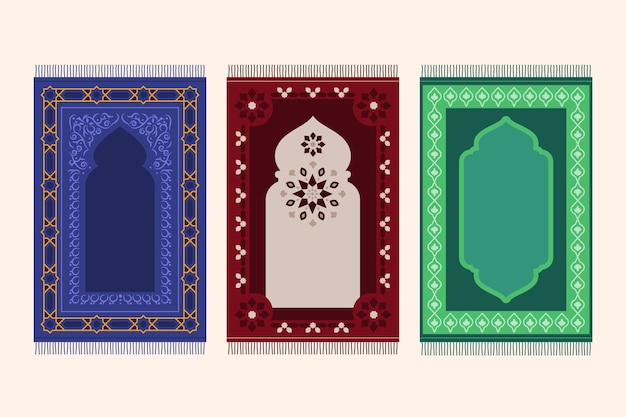
\includegraphics[width=1.26518in,height=2.06178in]{media/image1.jpeg} T
\_A\_ P \_E\_ T \_E\_

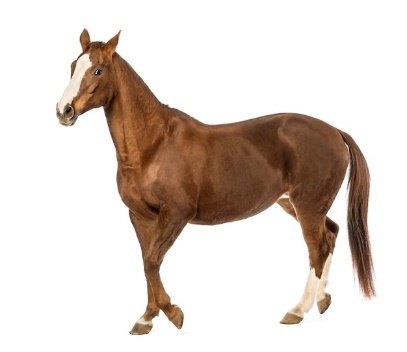
\includegraphics[width=1.85417in,height=1.60240in]{media/image2.jpeg}

C \_\_A\_ V \_\_A\_ L \_\_O\_


\includegraphics[width=1.57292in,height=1.57292in]{media/image3.jpeg}\_E\_\_
STR\_\_E\_\_ L\_\_A\_

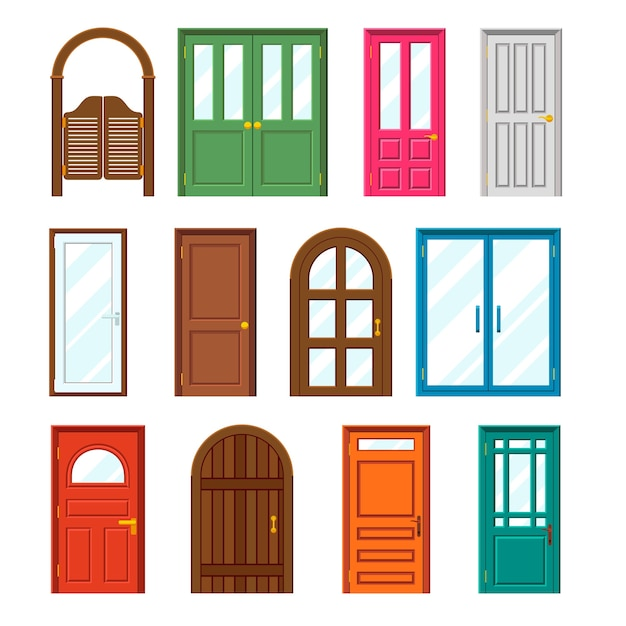
\includegraphics[width=1.27083in,height=1.80035in]{media/image4.jpeg}
P\_O\_\_RT \_\_A\_

%https://www.freepik.com/free-vector/hand-drawn-flat-design-prayer-mat-illustration\_22870006.htm\#page=2\&query=TAPETE\&position=0\&from\_view=search\&track=sph
%\url{https://www.freepik.com/premium-photo/horse-walking-front-white-background_19983860.htm?query=CAVALO\#from_view=detail_alsolike}
%\url{https://www.freepik.com/free-vector/golden-star-3d_830718.htm\#query=ESTRELA\&position=16\&from_view=search\&track=sph}
%https://www.freepik.com/free-vector/set-front-buildings-doors-flat-style\_11053573.htm\#query=PORTA\&position=12\&from\_view=search\&track=sph

Você completou as palavras com

\begin{boxlist}
\boxitem[] Vogais 

\boxitem[] Consoantes
\end{boxlist}

\coment{Apresente as vogais em cartaz. Pergunte o nome dos objetos 
representados nas imagens e, em seguida, convide as crianças para
montar as palavras no alfabeto móvel para identificar as letras faltantes.}

\num{2} Complete o alfabeto com as letras que estão faltado.

\begin{longtable}[]{@{}llllllll@{}}
\toprule
\textbf{A } & \textbf{B} & \textbf{C} & \textbf{D} & \textbf{E} &
\textbf{F} & \textbf{G} & H\tabularnewline
\midrule
\endhead
\textbf{I} & \textbf{J} & \textbf{K} & \textbf{L} & \textbf{M} &
\textbf{N} & \textbf{O} & P\tabularnewline
\textbf{Q} & \textbf{R} & \textbf{S} & \textbf{T} & \textbf{U} &
\textbf{V} & \textbf{W} & X\tabularnewline
\textbf{Y} & \textbf{Z}\tabularnewline
\bottomrule
\end{longtable}

Você completou as palavras com:

\begin{boxlist}
\boxitem[] Vogais 

\boxitem[] Consoantes
\end{boxlist}

\coment{Leve o alfabeto móvel para sala e convide os alunos para
organizar as letras na ordem certa. Em seguida, oriente-os a preencher
o quadro; depois ajude a separar vogais e consoantes.}

\num{3} Leia o poema.

\textbf{A vaca Filomena e a formiga Violeta}\\
Isabel Cristina Silveira Soares

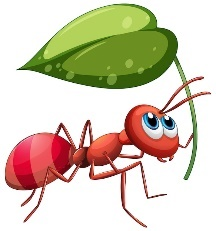
\includegraphics[width=0.97986in,height=1.05208in]{media/image5.jpeg}
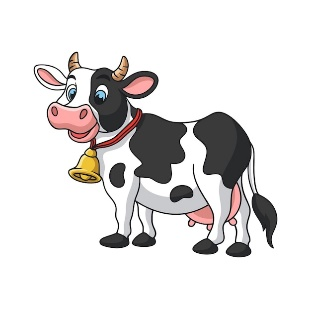
\includegraphics[width=1.16127in,height=0.95833in]{media/image6.jpeg}

\begin{verse}
A vaca Filomena\\
mora na vila formosa\\
A formiga Violeta\\
mora na cerca cor de rosa.

A vaca Filomena\\
come as uvas da parreira\\
A formiga Violeta\\
acha isto uma besteira.
\end{verse}

\fonte{https://seceducacao.padua.rj.gov.br/wp-content/uploads/2021/05/3o-ano-Ling.-Portuguesa-ATIV.17.pdf.
Acesso 28 de Fev 2023.}

Encontre e pinte no texto todas as palavras iniciadas com F e V. 
Depois escreva abaixo as palavras que encontrou.

\reduline{As palavras encontradas são as seguintes: vaca, Filomena, vila,
formosa, formiga, violeta.
Leve as palavras \textit{vaca} e \textit{formiga} em uma caixinha e
apresente-as para as crianças. Faça a leitura das palavras e estimule 
questionamentos sobre esses animais: os alunos sabem como eles são?
Onde esses animais vivem? Que sons eles emitem? Faça com os
alunos a leitura do poema e oriente a localização das palavras iniciadas
com as consoantes V e F.\hfill}

\num{4} Complete os espaços a seguir com as letras iniciais das palavras
\textit{violeta} e \textit{filomena}.

\coment{Leve as palavras Violeta e Filomena em um cartaz. Explore a 
letra inicial e o som da letra nas palavras.}


\includegraphics[width=1.01042in,height=1.55278in]{media/image7.jpeg}

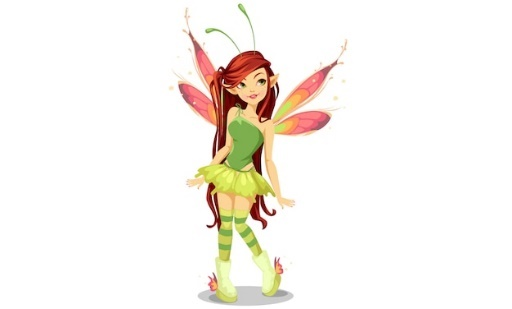
\includegraphics[width=0.87500in,height=1.40486in]{media/image8.jpeg}

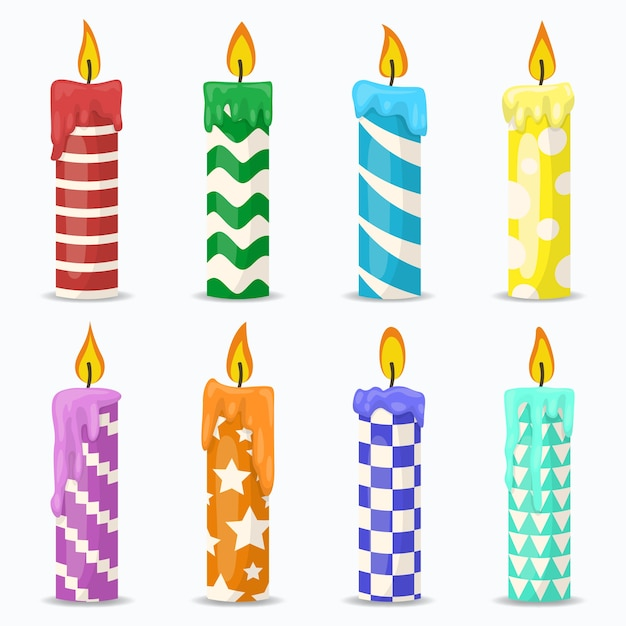
\includegraphics[width=0.56250in,height=1.32083in]{media/image9.jpeg}

\_\_V\_ELA \_FADA \_F\_ACA

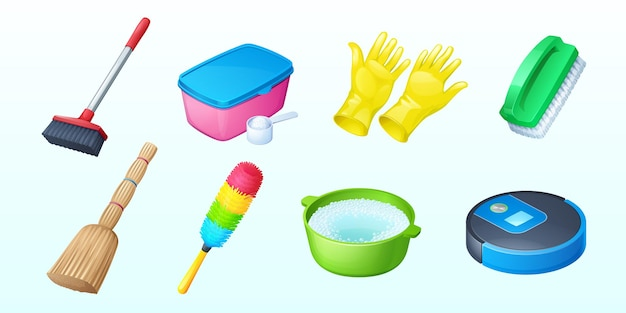
\includegraphics[width=1.12500in,height=1.48958in]{media/image10.jpeg}
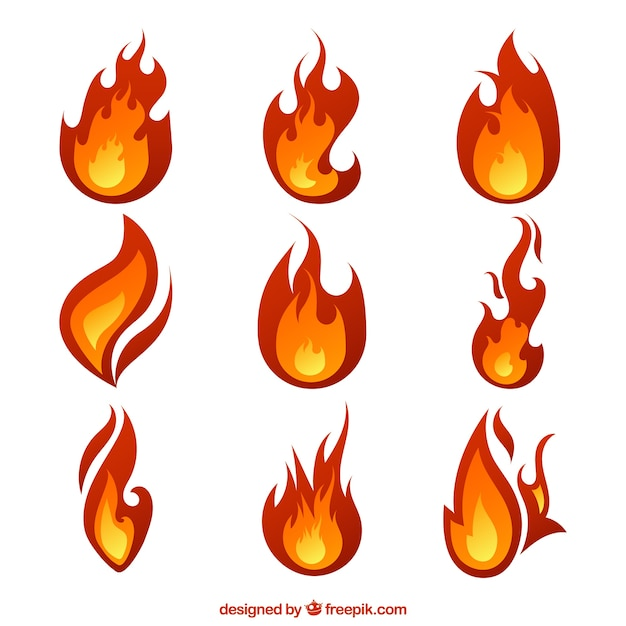
\includegraphics[width=1.34375in,height=1.77083in]{media/image11.jpeg}
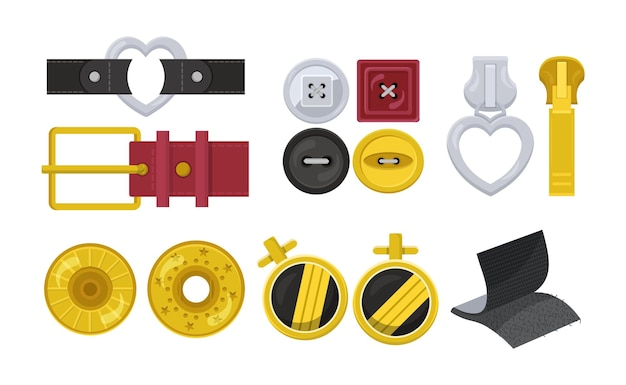
\includegraphics[width=1.77847in,height=0.76369in]{media/image12.jpeg}

\_\_\_F\_\_IVELA \_\_F\_\_OGO VASSOURA

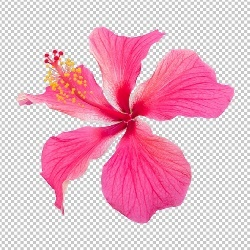
\includegraphics[width=1.13542in,height=1.13542in]{media/image13.jpeg}
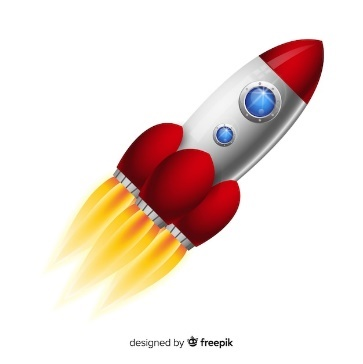
\includegraphics[width=1.24653in,height=1.22917in]{media/image14.jpeg}
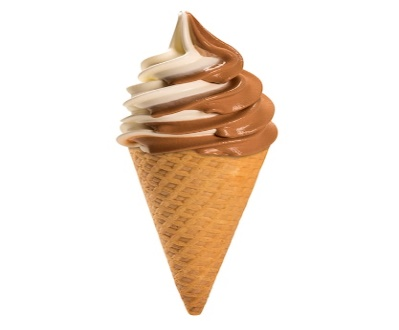
\includegraphics[width=1.00000in,height=1.49583in]{media/image15.jpeg}

SOR\_V\_ETE \_F\_\_OGUETE \_F \_LOR

%\url{https://www.freepik.com/free-vector/collection-christmas-candle-flat-design_6074662.htm\#page=2\&query=VELA\&position=28\&from_view=search\&track=sph}
%\url{https://www.freepik.com/search?format=search\&query=FADA}
%\url{https://www.freepik.com/premium-psd/3d-knife-icon-render-isolated_20395607.htm\#page=4\&query=FACA\&position=17\&from_view=search\&track=sph}
%\url{https://www.freepik.com/free-vector/clasps-design-elements-set-isolated-white-carabiner-hook-snap-bag-belt-buckle-leather-tabs-straps-cufflinks-buttons-different-shapes-materials_27398885.htm\#query=FIVELA\&position=23\&from_view=search\&track=sph}
%https://www.freepik.com/free-vector/great-flames-with-different-designs\_1086041.htm\#query=FOGO\&position=21\&from\_view=search\&track=sph
%\url{https://www.freepik.com/free-vector/cleaning-icons-with-broom-vacuum-cleaner_16956931.htm\#page=2\&query=VASSOURA\&position=7\&from_view=search\&track=sph}
%\url{https://www.freepik.com/premium-photo/vanilla-chocolate-soft-ice-cream-waffled-cone_9043953.htm\#page=3\&query=SORVETE\&position=24\&from_view=search\&track=sph}
%\url{https://www.freepik.com/free-vector/modern-space-rocket-with-realistic-design_2825905.htm\#query=FOGUETE\&position=32\&from_view=search\&track=sph}
%https://www.freepik.com/premium-psd/pink-hibiscus-flower-isolated-rendering\_15458965.htm?query=FLOR\#from\_view=detail\_alsolike

\num{5} Pinte as iniciais de cada palavra.

\coment{Leve para sala palavras iniciadas pelas letras T, D, F, V, B, P. 
Convide as crianças para fazer a leitura, identificado o som das letras
iniciais e finais, e quantidade de sílabas. Também é possível trabalhar
a função social da escrita das palavras}.

\begin{tabular}{|c|c|c|c|c|}
\hline
\textbf{VACINA} & F & T & D & V \\ \hline
\textbf{TESOURA} & P & D & T & F \\ \hline
\textbf{VASSOURA} & B & T & V & F \\ \hline
\textbf{FACA} & V & F & D & T \\ \hline
\textbf{DEDO} & T & V & F & D \\ \hline
\textbf{PANELA} & V & T & P & B \\ \hline
\textbf{DOMINÓ} & B & D & T & P \\ \hline
\textbf{BONECA} & F & P & B & D \\ \hline
\end{tabular}

\num{6} Numere os desenhos conforme os números das palavras.

\coment{Faça leitura das palavras com as crianças, de modo que elas
identifiquem a numeração e façam a associação correta.}

\begin{longtable}[]{@{}llll@{}}
\toprule
\begin{minipage}[b]{0.24\columnwidth}\raggedright\strut
\textbf{1- BOLA}

\textbf{2- FOCA}

\textbf{3- TATU}

\textbf{4- PANELA}

\textbf{5- TAPETE}\strut
\end{minipage} & \begin{minipage}[b]{0.24\columnwidth}\raggedright\strut
\textbf{6- FORMIGA}

\textbf{7- DADO}

\textbf{8- VACA}

\textbf{9- PATO}

\textbf{10- BONECA}\strut
\end{minipage}\tabularnewline
\midrule
\endhead
\textbf{\_\_10\_-} &

\includegraphics[width=1.16667in,height=0.96319in]{media/image16.jpeg} &
\textbf{\_\_8\_\_} &
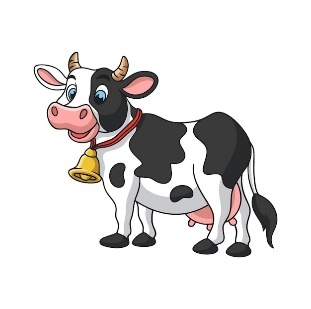
\includegraphics[width=1.16127in,height=0.95833in]{media/image17.jpeg}\tabularnewline
\textbf{\_\_\_2\_} &
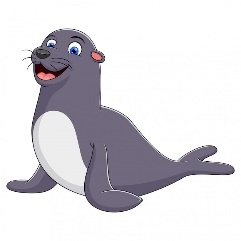
\includegraphics[width=1.09375in,height=1.09375in]{media/image18.jpeg} &
\textbf{\_\_4\_\_} &
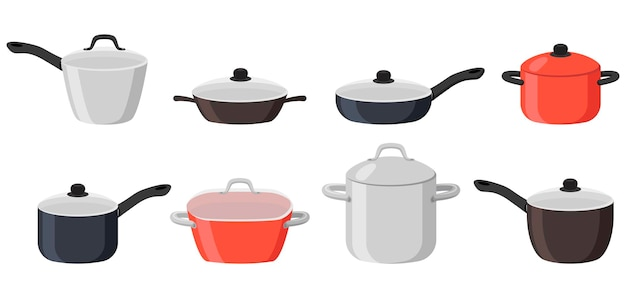
\includegraphics[width=1.27986in,height=0.98958in]{media/image19.jpeg}\tabularnewline
\textbf{\_\_T\_\_} &
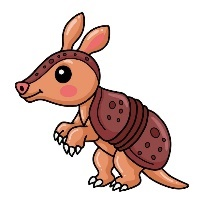
\includegraphics[width=0.92708in,height=0.92708in]{media/image20.jpeg} &
\textbf{\_\_F\_\_} &
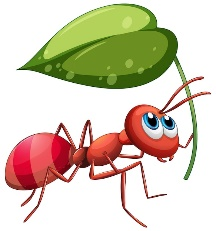
\includegraphics[width=0.97986in,height=1.05208in]{media/image21.jpeg}\tabularnewline
\textbf{\_\_\_B\_} &
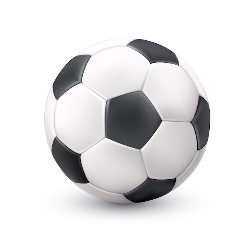
\includegraphics[width=1.13542in,height=1.13542in]{media/image22.jpeg} &
\textbf{\_D\_\_\_} &
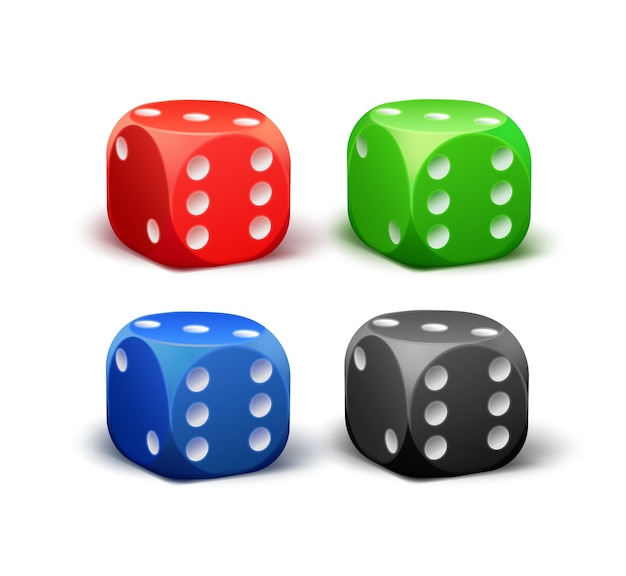
\includegraphics[width=1.23958in,height=1.15833in]{media/image23.jpeg}\tabularnewline
\textbf{\_\_\_P\_} &
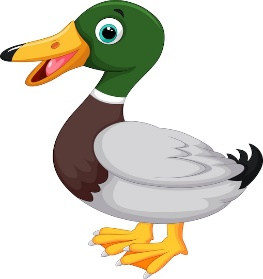
\includegraphics[width=1.19722in,height=1.27083in]{media/image24.jpeg} &
\textbf{\_\_T\_\_} &
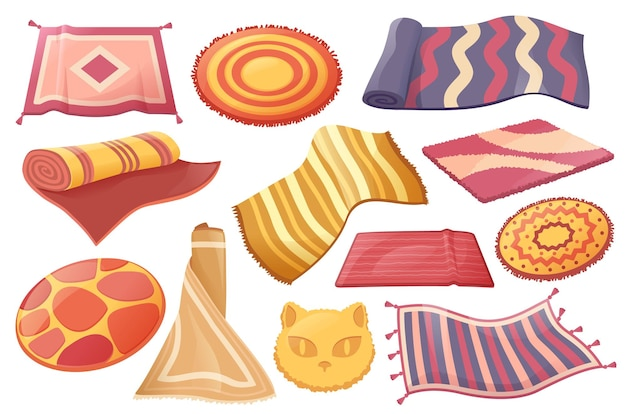
\includegraphics[width=2.21875in,height=1.11458in]{media/image25.jpeg}\tabularnewline
\bottomrule
\end{longtable}

%https://www.freepik.com/premium-vector/pink-chibi-girl\_9687656.htm\#query=BONECA\&position=34\&from\_view=search\&track=sph
%\url{https://www.freepik.com/premium-vector/cartoon-illustration-cool-cow_17447402.htm\#page=2\&query=VACA\&position=48\&from_view=search\&track=sph}
%https://www.freepik.com/premium-vector/seal-cartoon-isolated\_6122224.htm\#query=FOCA\&position=36\&from\_view=search\&track=sph
%\url{https://www.freepik.com/free-vector/frying-pans-saucepans-cartoon-illustration-set-metal-cooking-pots-with-lid-different-sizes-stainless-utensils-making-soup-boiling-water-household-kitchen-concept_26921753.htm\#query=PANELA\&position=1\&from_view=search\&track=sph}
%https://www.freepik.com/premium-vector/cute-little-armadillo-cartoon-standing\_27006356.htm\#query=TATU\&position=13\&from\_view=search\&track=sph
%\url{https://www.freepik.com/free-vector/ant-holding-green-leaf_19589093.htm\#query=FORMIGA\&position=4\&from_view=search\&track=sph}
%\url{https://www.freepik.com/premium-vector/cartoon-wool-carpets-bath-rug-woven-mat-carpet-roll-home-floor-textile-decor-vector-illustration-set_28995572.htm\#page=2\&query=TAPETE\&position=43\&from_view=search\&track=sph}
%\url{https://www.freepik.com/premium-vector/cute-cartoon-duck_3219176.htm\#query=PATO\&position=8\&from_view=search\&track=sph}
%https://www.freepik.com/free-vector/soccer-ball-realistic-white-black-picture\_2875610.htm\#query=bola\&position=1\&from\_view=search\&track=sph

\num{7} Complete as palvaras com \textbf{-ca -co -cu} ou \textbf{-qua -que -qui}.

\coment{Convide as crianças a falar o nome das imagens para identificar a grafia da palavra.}


\includegraphics[width=1.30278in,height=0.81667in]{media/image26.jpeg}
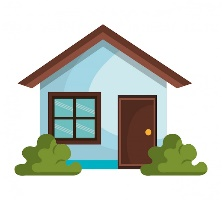
\includegraphics[width=1.00903in,height=0.90972in]{media/image27.jpeg}

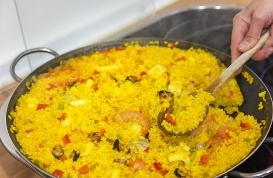
\includegraphics[width=1.24028in,height=0.81042in]{media/image28.jpeg}
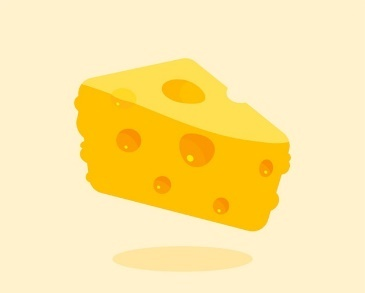
\includegraphics[width=1.05556in,height=0.81667in]{media/image29.jpeg}

CASA QUEI\_\_\_\_\_IJO CU \_\_\_\_\_\_\_SCUS CU\_TIA

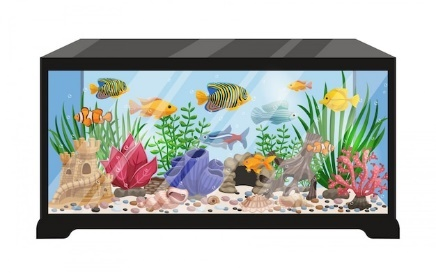
\includegraphics[width=1.98343in,height=1.24038in]{media/image30.jpeg}
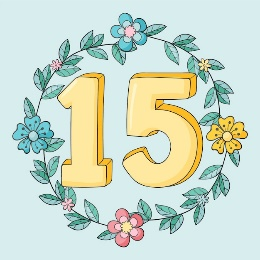
\includegraphics[width=1.18269in,height=1.18269in]{media/image31.jpeg}

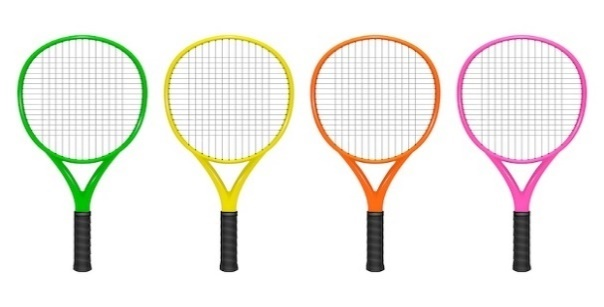
\includegraphics[width=0.70192in,height=1.39623in]{media/image32.jpeg}

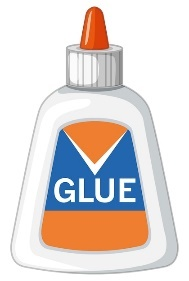
\includegraphics[width=0.85819in,height=1.27885in]{media/image33.jpeg}

QUI\_\_\_NZE Á \_\_QUA\_\_RIO CO\_\_\_LA RA\_QUE\_TE

%https://www.freepik.com/free-vector/beautiful-home\_4979878.htm\#query=CASA\&position=27\&from\_view=search\&track=sph
%https://www.freepik.com/free-vector/cheese-isolated-cartoon-art-illustration\_14478854.htm\#query=QUEIJO\&position=3\&from\_view=search\&track=sph
%https://www.flickr.com/photos/gjshepherd/18994508411
%https://www.freepik.com/free-vector/hand-drawn-15th-anniversary-birthday\_22751030.htm\#query=N\%C3\%9AMERO\%2015\&position=6\&from\_view=search\&track=ais
%https://www.freepik.com/free-vector/aquarium-tank-cartoon-illustration\_5971410.htm\#query=AQUARIO\&position=34\&from\_view=search\&track=sph
%https://www.freepik.com/free-vector/bottle-latex-glue\_19589095.htm\#query=COLA\&position=0\&from\_view=search\&track=sph

\num{8} Encontre a sílaba mais forte e complete com O ou U.

\coment{Leve para a classe uma caixinha enfeitada com palavras terminadas
com O e U. Passe a caixinha para os alunos em círculo, ao som de uma 
música. Quando a música parar, o aluno que estiver com a caixinha na 
mão deve ler a palavra observando a letra  final. Em seguida, convide
toda a turma a pronunciar a palavra e, então, descobrir a sílaba forte.
Explique como descobrir quando a sílaba é forte e fraca, ensinando que,
quando o U está no final, ele é sempre forte, e que o O é sempre fraco
no final das palavras.}

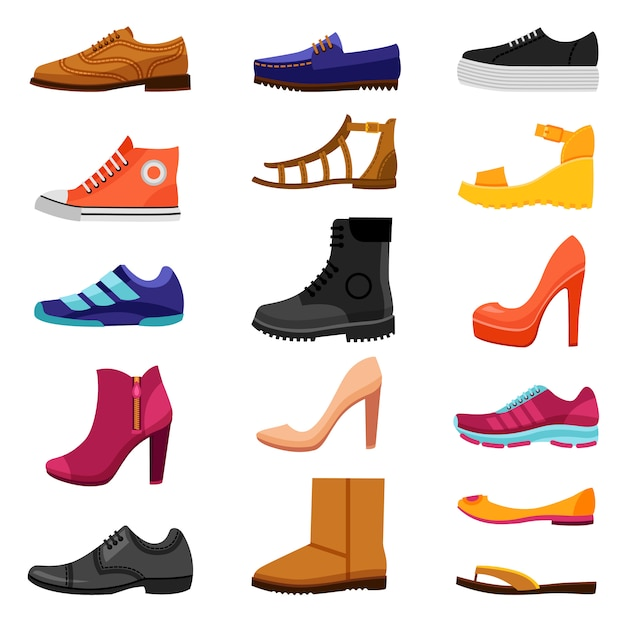
\includegraphics[width=1.65486in,height=0.74499in]{media/image34.jpeg}
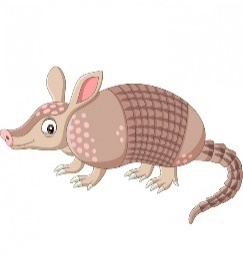
\includegraphics[width=1.09512in,height=0.74522in]{media/image35.jpeg}
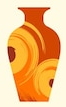
\includegraphics[width=0.69978in,height=1.10152in]{media/image36.jpeg}

TAT\_\_U\_\_ VAS\_O\_\_ SAPAT\_\_O\_\_


\includegraphics[width=0.59861in,height=1.03542in]{media/image37.jpeg}

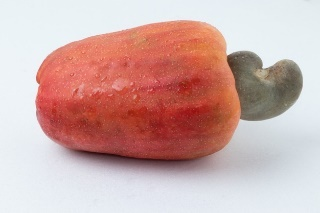
\includegraphics[width=1.26250in,height=0.68750in]{media/image38.jpeg}
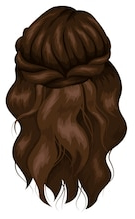
\includegraphics[width=0.59873in,height=0.93296in]{media/image39.jpeg}

CABEL\_\_O\_ CAJ\_\_U\_\_ ESPELH\_O\_\_

%https://www.freepik.com/premium-vector/cartoon-armadillo-white\_6408471.htm\#query=TATU\&position=27\&from\_view=search\&track=sph
%\url{https://www.freepik.com/premium-photo/fresh-cashew-isolated-white-background_18591010.htm\#page=6\&query=CAJU\&position=5\&from_view=search\&track=sph}
%\url{https://www.freepik.com/free-vector/contemporary-ceramic-vases-modern-jugs-pots_29836873.htm\#query=VASO\&position=21\&from_view=search\&track=sph}
%\url{https://www.freepik.com/free-vector/women-wigs-hairstyle-realistic-icons-set_4016983.htm\#page=3\&query=CABELO\&position=49\&from_view=search\&track=sph}
%\url{https://www.freepik.com/free-vector/footwear-colored-icons-set_4431156.htm\#query=SAPATO\&position=1\&from_view=search\&track=sph}
%https://www.freepik.com/free-vector/sticker-template-pink-mirror-with-handle-isolated\_20721062.htm\#query=ESPELHO\&position=12\&from\_view=search\&track=sph

\num{9} Pinte as palvras escritas com C que tem o som de S.
%Felipe: aqui precisamos padronizar, como comentei anteriormente. 

\coment{Leve para sala palavras escritas com C. Organize uma roda de
conversa na qual você orientará os alunos a organizar as palavras de
acordo com a vogal que acompanha a letra C. Em seguida, explique a 
regra para descobrir se o C tem som de K ou S.}

\begin{longtable}[]{@{}lllll@{}}
\toprule
\textbf{CINEMA} & \textbf{CASA} & \textbf{CISNE} & \textbf{CEGO} &
\textbf{COCADA}\tabularnewline
\midrule
\endhead
\textbf{CADEIRA} & \textbf{CARRO} & \textbf{CINTO } & \textbf{COCO} &
\textbf{CAMA}\tabularnewline
\bottomrule
\end{longtable}

\num{10} Troque as letras e forme outras palavras.

\coment{Utilize o alfabeto móvel com as palavras
solicitadas no exercício e outras. Também é possível fazer a 
brincadeira da forca.}

\begin{longtable}[]{@{}lll@{}}
\toprule
\textbf{V POR F} & \textbf{D POR T} & \textbf{B POR P}\tabularnewline
\midrule
\endhead
\textbf{VACA} & \textbf{DADO} & \textbf{BODE}\tabularnewline
\textbf{\_F\_ACA} & \textbf{TATO} & \textbf{\_\_P\_ODE}\tabularnewline
\textbf{VILA} & \textbf{DIA} & \textbf{BOTE}\tabularnewline
\textbf{\_F\_I LA} & \textbf{\_T\_IA} & \textbf{\_P\_OTE}\tabularnewline
\bottomrule
\end{longtable}

\num{11} Complete a cruzadinha com o nome das figuras.

\coment{Explore as frutas e legumes da atividade, fazendo 
questionamentos. Monte as palavras no alfabeto móvel com as crianças.
Em seguida, oriente a escrita na cruzadinha.}

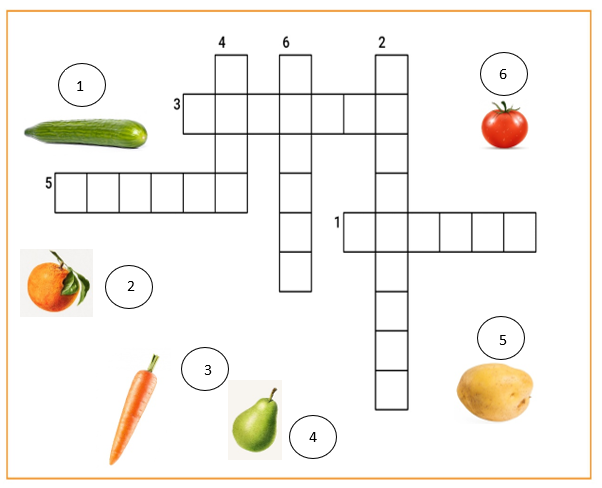
\includegraphics[width=5.69167in,height=4.10139in]{media/image40.png}

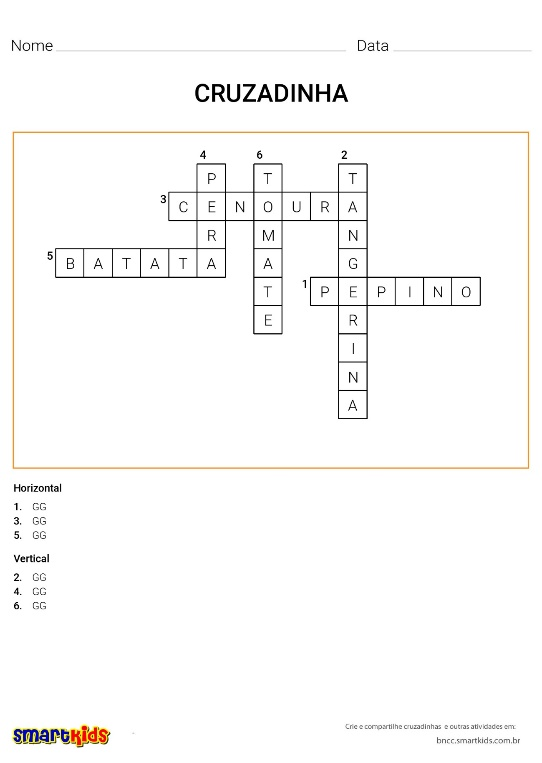
\includegraphics[width=2.40385in,height=1.79075in]{media/image41.jpeg}

Resposta da cruzadinha

%\url{https://www.freepik.com/free-photo/green-cucumber_7399055.htm?query=PEPINO\#from_view=detail_alsolike}
%\url{https://www.freepik.com/free-vector/hand-drawn-natural-fresh-oranges-set_16351577.htm\#query=tangerina\&position=44\&from_view=search\&track=sph}
%\url{https://www.freepik.com/premium-photo/fresh-carrot-isolated-white_9544212.htm\#page=2\&query=CENOURA\&position=16\&from_view=search\&track=sph}
%\url{https://www.freepik.com/free-vector/vintage-pear-illustration_16279755.htm\#query=PERA\&position=1\&from_view=search\&track=sph}
%\url{https://www.freepik.com/free-photo/potato_1025630.htm\#query=BATATA\&position=2\&from_view=search\&track=sph}
%https://www.freepik.com/free-vector/fresh-tomato\_957857.htm\#query=TOMATE\&position=17\&from\_view=search\&track=sph

\num{12} Encontre e pinte as palavras no diagrama.

\coment{Depois da leitura das palavras, oriente os alunos a localizá-las
no diagrama.}

\begin{longtable}[]{@{}llllllll@{}}
\toprule
TATU- CABELO - BONECA- PANELA- CAJU - FADA- DADO - VASO -- CAMA --
TAPETE\tabularnewline
\midrule
\endhead
D & B & F & A & D & A & D & G\tabularnewline
A & C & A & B & E & L & O & U\tabularnewline
G & Y & B & O & C & A & M & A\tabularnewline
S & T & I & N & H & M & A & Q\tabularnewline
P & A & N & E & L & A & D & F\tabularnewline
H & T & O & C & A & J & U & L\tabularnewline
J & U & K & A & D & A & D & O\tabularnewline
T & A & P & E & T & E & Z & X\tabularnewline
K & V & A & S & O & B & G & J\tabularnewline
\bottomrule
\end{longtable}

\colorsec{Treino}

\num{1} Observe o animal que Júlia encontrou enquanto brincava na 
fazenda do Tio Belo.


\includegraphics[width=1.36528in,height=1.64861in]{media/image42.jpeg}

%\url{https://www.freepik.com/premium-vector/set-ants-carry-leaf-stone-tree-branches-white_9221745.htm?query=formiga\#from_view=detail_alsolike}
%Acesso 01 mar. 2023.

A palavra que começa com a mesma letra do nome do animal que Júlia
encontrou é

\begin{minipage}{.5\textwidth}
\begin{escolha}
\item vaso.

\item gato.

\item bola.

\item foca
\end{escolha}
\end{minipage}
\sidetext{SAEB: Relacionar elementos sonoros das palavras com sua
representação escrita

BNCC: EF02LP03 -- Ler e escrever palavras com correspondências
regulares diretas entre letras e fonemas (f, v, t, d, p, b) e
correspondências~regulares contextuais (c e q; e e o, em posição átona
em final de palavra).}

a) Incorreta. O animal encontrado por Júlia é uma \textit{formiga}, 
que começa com a letra F, não com a letra V.
b) Incorreta. O animal encontrado por Júlia é uma \textit{formiga}, 
que começa com a letra F, não com a letra G.
c) Incorreta. O animal encontrado por Júlia é uma \textit{formiga}, 
que começa com a letra F, não com a letra B. 
d) Correta. Tanto \textit{formiga} quanto \textit{foca} são palavras
que começam com a letra F.

\num{2} Observe a palavra que Tiago leu para sua professora.

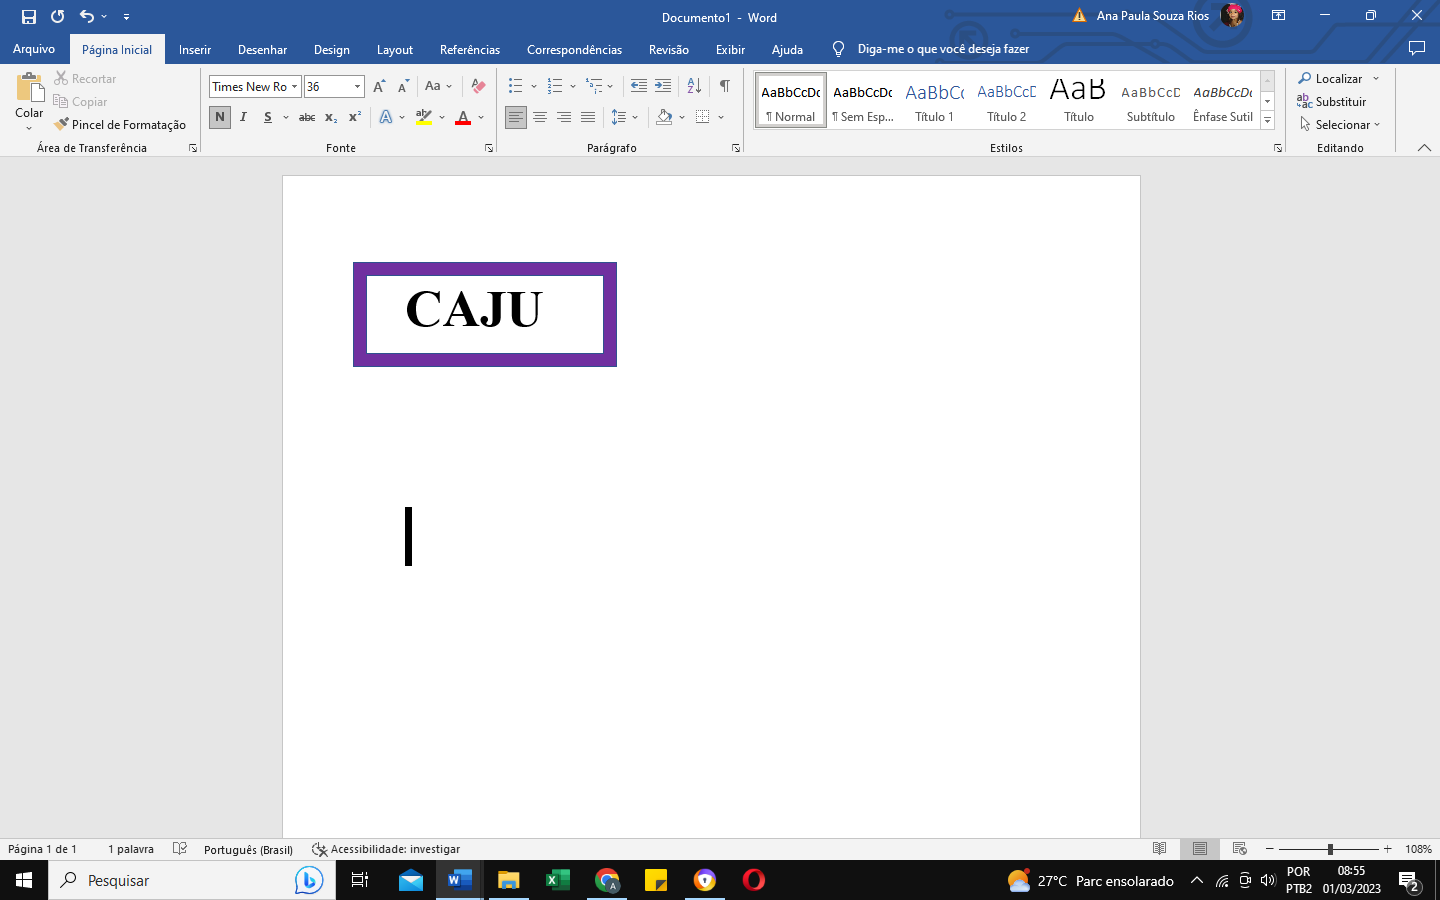
\includegraphics[width=2.79792in,height=1.15833in]{media/image43.png}

O nome da figura que termina com a mesma letra da palavra que Tiago leu é

\begin{escolha}
\item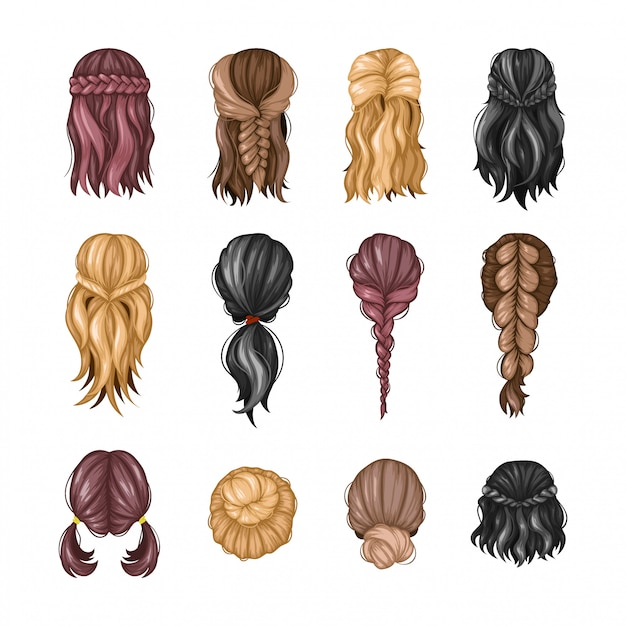
\includegraphics[width=0.79792in,height=0.81667in]{media/image44.jpeg}

\item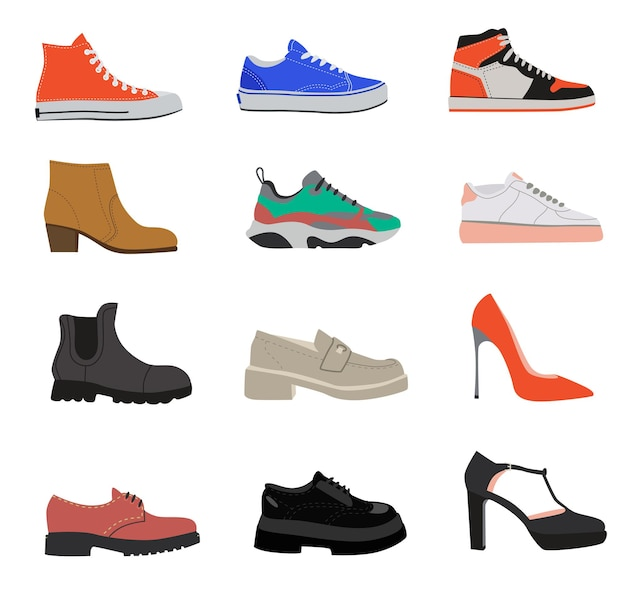
\includegraphics[width=1.02847in,height=0.72292in]{media/image45.jpeg}

\item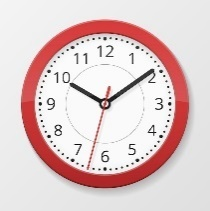
\includegraphics[width=0.79792in,height=0.79931in]{media/image46.jpeg}

\item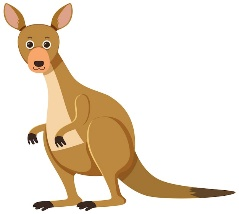
\includegraphics[width=1.08611in,height=0.97222in]{media/image47.jpeg}
\end{escolha}

\coment{SAEB: Relacionar elementos sonoros das palavras com sua
representação escrita

BNCC: EF02LP03 -- Ler e escrever palavras com correspondências
regulares diretas entre letras e fonemas (f, v, t, d, p, b) e
correspondências~regulares contextuais (c e q; e e o, em posição átona
em final de palavra).}

a) Incorreta. \textit{Caju} termina com a letra U, mas \textit{cabelo} termina com a letra O.

b) Incorreta. \textit{Caju} termina com a letra U, mas \textit{sapato} termina com a letra O.

c) Incorreta. \textit{Caju} termina com a letra U, mas \textit{relógio} termina com a letra O.

(D) Correta. As palavras \textit{caju} e \textit{canguru} terminam com a letra U.

%\url{https://www.freepik.com/premium-vector/set-variety-women-hairstyles_7719339.htm\#from_view=detail_alsolike}
%\url{https://www.freepik.com/free-vector/random-female-shoes-flat-illustrations-set-summer-autumn-winter-foot-wear-women-moccasins-boots-trainers-heels-isolated-white_20827876.htm\#query=SAPATO\&position=1\&from_view=search\&track=sph}
%\url{https://www.freepik.com/free-vector/round-wall-quartz-clock-red-color-isolated-white-background_13031909.htm\#query=RELOGIO\&position=27\&from_view=search\&track=sph}
%https://www.freepik.com/free-vector/kangaroo-cartoon-character-isolated\_29098402.htm\#query=CANGURU\&position=7\&from\_view=search\&track=sph

\num{3} Observe o presente que Bruna ganhou.

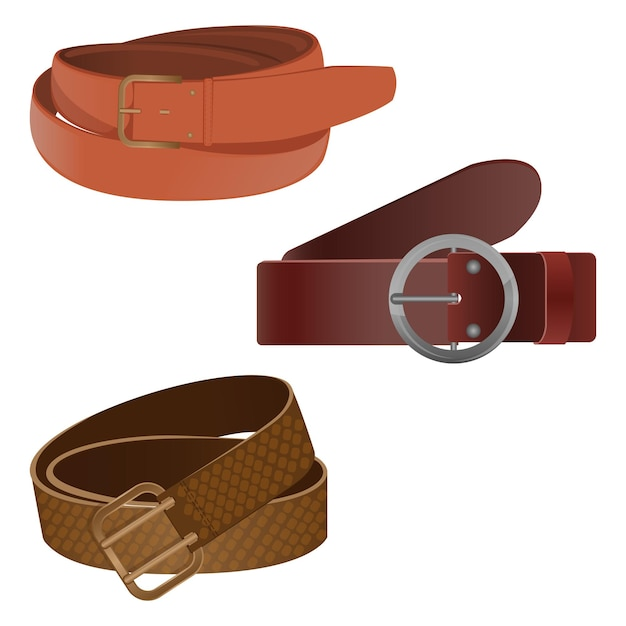
\includegraphics[width=3.62413in,height=2.01875in]{media/image48.jpeg}

%\url{https://www.freepik.com/premium-vector/set-leather-waist-belts-isolated-background_13798858.htm\#query=CINTO\&position=38\&from_view=search\&track=sph}
%Acesso 01 mar. 2023.

A palavra que começa como o mesmo som da letra do nome do presente de Bruna é

\begin{minipage}{.5\textwidth}
\begin{escolha}
\item cama.

\item cubo.

\item cebola.

\item cocada.
\end{escolha}
\end{minipage}
\sidetext{SAEB: Relacionar elementos sonoros das palavras com sua
representação escrita.

BNCC: EF02LP03 -- Ler e
escrever palavras com correspondências~regulares diretas entre letras e
fonemas (f, v, t, d, p, b) e correspondências~regulares contextuais (c e
q; e e o, em posição átona em final de palavra).}

a) Incorreta. A letra C da palavra \textit{Cinto} tem som de S, mas,
na palavra \textit{cama}, essa letra tem som de K. 
b) Incorreta. A letra C da palavra \textit{Cinto} tem som de S, mas,
na palavra \textit{cubo}, essa letra tem som de K.
c) Correta. A letra C das palavras \textit{Cinto} e \textit{cebola}
têm som de S.
d) Incorreta. A letra C da palavra \textit{Cinto} tem som de S, mas,
na palavra \textit{cocada}, essa letra tem som de K.

\chapter{Lendo e escrevendo}
\markboth{Módulo 2}{}

\coment{Habilidades da BNCC: EF02LP04, EF02LP05}

\colorsec{Habilidades do SAEB}

\begin{itemize}
\item Ler palavras.
\item Escrever palavras.
\item Ler frases.
\end{itemize}

\conteudo{Para escrever uma palavra, você precisa usar as letras que
são chamadas de vogais e as consoantes.

%Paulo: é o caso de, na explicação abaixo, colocar as vogais e consoantes em destaque, dentro de um box, em fonte grande e caixa alta 

As vogais são \textbf{A -- E -- I -- O -- U} 

e as consoantes são \textbf{B -- C -- D -- F -- G -- H -- J -- K -- L -- M -- N -- P -- Q -- R -- S
-- T -- V -- W -- Y -- X -- Z.}

As palavras são lidas e escritas da esquerda para a direita.

%Paulo, atenção: no original, existe uma seta indicando o sentido da leitura das palavras abaixo

\textbf{GRAVIOLA LÂMPADA AVIÃO LARANJA }

Existem diferentes maneiras de compor a sílaba de uma palavra. 

\textbf{CONSOANTE + VOGAL}: é o que acontece nas três sílabas das 
palavras \textit{sapato} e \textit{telefone}: SA-PA-TO e TE-LE-FO-NE

\textbf{VOGAL}: é o que acontece na segunda sílaba das  
palavras \textit{saída} e \textit{saúde}: SA-Í-DA e SA-Ú-DE

\textbf{CONSOANTE + VOGAL + CONSOANTE}: é o que acontece na 
primera sílaba das palavras \textit{porta} e \textit{cortina}:
POR-TA e COR-TI-NA

\textbf{CONSOANTE + CONSOANTE + VOGAL}: é o que acontece na 
primera sílaba da palavra \textit{criança} e na última
sílaba da palavra \textit{livro}: CRI-AN-ÇA e LI-VRO 

Observe o quadro abaixo, com outros exemplos:

\begin{longtable}[]{@{}lllll@{}}
\toprule
\textbf{PALAVRAS} & \textbf{FORMAÇÃO SILÁBICA CV} & \textbf{FORMAÇÃO
SILÁBICA V} & \textbf{FORMAÇÃO SILÁBICA CVC} & \textbf{FORMAÇÃO SILÁBICA
CCV}\tabularnewline
\midrule
\endhead
\textbf{GRAVIOLA} & GRA- \textbf{VI}- O-\textbf{LA} & GRA- VI-
\textbf{O}-LA & \textbf{*} & \textbf{GRA}- VI- O-LA\tabularnewline
\textbf{LÂMPADA} & LÂM -- \textbf{PA - DA} & * & \textbf{LÂM}--PA - DA &
*\tabularnewline
\textbf{AVIÂO} & A -- \textbf{VI} - ÂO & \textbf{A} -- VI - ÂO & * &
*\tabularnewline
\textbf{LARANJA} & \textbf{LA}-RAN-\textbf{JÁ} & * & LA-\textbf{RAN}-JÁ
& *\tabularnewline
\bottomrule
\end{longtable}

Note que, em todas as formações das sílabas, aparecem vogais. Isso
acontece porque não existe sílaba sem vogal, isto é, uma  sílaba não
se forma só com consoantes.

Observe a frase a seguir:

\textbf{O avião pousou cedo.}

Você conhece esse sinal em cima da letra A da palavra \textbf{avião}?

Esse sinal é o \textbf{til}, usado nas vogais A e O para marcar a
nasalidade presente na sílaba.

As marcas de nasalidade aparece também nas letras M e N, no final da
sílaba. É o que acontece, por exemplo, com as seguintes palavras:

\textbf{LÂMPADA E LARANJA}

A letra \textbf{M} é utilizada antes das consoantes P e B.  
A letra \textbf{N} é usada antes das demais consoantes, nunca 
no final das palavras.
}

\colorsec{Atividades}

\num{1} Escreva os nomes das figuras.

\coment{Leve o alfabeto móvel para a sala de 
aula. Convide as crianças para manusear as letras; em seguida, 
oriente-as a formar as palavras que nomeiam as figuras. Sugira a elas
que, antes de escrever, elas devem pronunciar a palavra, escrevendo-a 
por sílabas ou pedacinhos.}

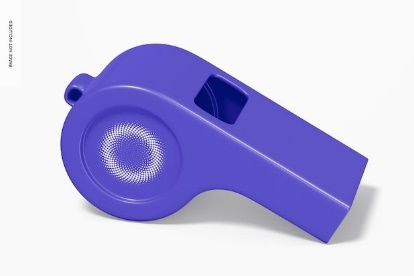
\includegraphics[width=1.46154in,height=0.93603in]{media/image49.jpeg}
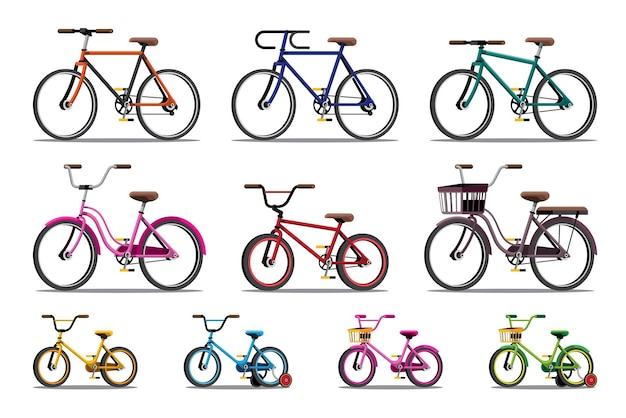
\includegraphics[width=1.16587in,height=0.93269in]{media/image50.jpeg}
\includegraphics[width=1.42308in,height=1.21950in]{media/image51.jpeg}

\reduline{Apito\hfill}

\reduline{Bicicleta\hfill}

\reduline{Árvore\hfill}

\includegraphics[width=1.10833in,height=1.00903in]{media/image52.jpeg}
\includegraphics[width=0.85556in,height=0.92222in]{media/image53.jpeg}
\includegraphics[width=0.79808in,height=0.79808in]{media/image54.jpeg}

\reduline{Bola\hfill}

\reduline{Raposa\hfill}

\reduline{Gaiola\hfill}

\includegraphics[width=0.91319in,height=1.16319in]{media/image55.jpeg}
\includegraphics[width=1.62569in,height=1.25000in]{media/image56.jpeg}
\includegraphics[width=0.93990in,height=1.27885in]{media/image57.jpeg}

\reduline{Pera\hfill}

\reduline{Pedra\hfill}

\reduline{Unha\hfill}

%\url{https://www.freepik.com/premium-psd/plastic-whistle-mockup_13956504.htm\#page=2\&query=apito\&position=33\&from_view=search\&track=sph}
%\url{https://www.freepik.com/free-vector/various-models-styles-bikes-riders-choose-from-according-age-usage-vector-cartoon-illustration-bicycle-isolated-white-background_23248359.htm\#query=bicicleta\&position=41\&from_view=search\&track=sph}
%\url{https://www.freepik.com/free-vector/tree_6132448.htm\#query=arvore\&position=12\&from_view=search\&track=sph}
%\url{https://www.freepik.com/free-vector/vector-isolated-realistic-soccer-ball-white_10601489.htm\#query=bola\&position=5\&from_view=search\&track=sph}
%\url{https://www.freepik.com/free-vector/hand-drawn-fox-collection_9468869.htm\#page=2\&query=raposa\&position=4\&from_view=search\&track=sph}
%\url{https://www.freepik.com/premium-photo/close-up-guava-fruit-pink-fresh-organic-with-leaves-whole-sliced-isolated-white-background-front-view_3766358.htm\#query=graviola\&position=33\&from_view=search\&track=sph}
%\url{https://www.freepik.com/free-vector/stones-rocks-cartoon_13050167.htm\#query=pedra\&position=11\&from_view=search\&track=sph}
%https://www.freepik.com/free-vector/illustration-nails-with-nail-polish-without-nail-polish\_11053390.htm\#query=unha\&position=11\&from\_view=search\&track=sph

\num{2} Separe as sílabas das palavras, depois circule as sílabas formadas por
consoante + consoante + vogal.

\coment{Leia as palavras com os alunos, 
orientando-os a identificar vogais e consoantes. Também é possível 
montar algumas palavras com o alfabeto móvel. Em seguida, peça a eles 
que batam palmas cada vez que um pedacinho da palavra for pronunciado.}

\begin{longtable}[]{@{}ll@{}}
\toprule
\textbf{PRATO} & Pra - to\tabularnewline
\midrule
\endhead
\textbf{FORMIGA} & For- mi -ga\tabularnewline
\textbf{BRAÇO} & Bra -ço\tabularnewline
\textbf{DRAGÃO} & Dra- gão\tabularnewline
\textbf{CRAVO} & Cra -- vo\tabularnewline
\bottomrule
\end{longtable}

\num{3} Ligue as palavras com seu desenho.

\coment{Leve para sala as palavras dentro de uma sacola. Cada criança
deve pegar uma palavra da sacola para fazer a leitura. Depois proponha
a atividade.}

Bicicleta

\includegraphics[width=0.38403in,height=0.53889in]{media/image59.png}

Janela

\includegraphics[width=0.60069in,height=0.48056in]{media/image60.png}

Borboleta

\includegraphics[width=0.49028in,height=0.40833in]{media/image61.png}

Dragão

\includegraphics[width=0.74931in,height=0.52292in]{media/image62.png}

Avião

\includegraphics[width=0.68542in,height=0.66319in]{media/image63.png}

\includegraphics[width=0.53403in,height=0.56667in]{media/image64.jpeg}

Prego

\includegraphics[width=0.91319in,height=0.52292in]{media/image65.png}

PIÃO

\includegraphics[width=0.65385in,height=0.73262in]{media/image66.png}

MANGA

Pomba

%\url{https://www.freepik.com/free-vector/various-models-styles-bikes-riders-choose-from-according-age-usage-vector-cartoon-illustration-bicycle-isolated-white-background_23248359.htm\#query=BICICLETA\&position=44\&from_view=search\&track=sph}
%\url{https://www.freepik.com/free-vector/hand-drawn-dove-outline-illustration_22340867.htm\#query=pomba\&position=1\&from_view=search\&track=sph}
%\url{https://www.freepik.com/free-photo/mango-table_6901195.htm\#query=manga\&position=1\&from_view=search\&track=sph}
%\url{https://www.freepik.com/free-vector/butterfly-collection_3980202.htm\#query=borboleta\&position=19\&from_view=search\&track=sph}
%\url{https://www.freepik.com/free-vector/different-kind-dinosaurs_22717262.htm\#query=dinossauro\&position=4\&from_view=search\&track=sph}
%\url{https://www.freepik.com/free-vector/wooden-windows-with-open-shutters-mediterranean-style-white_12569303.htm\#query=janela\&position=34\&from_view=search\&track=sph}
%\url{https://www.freepik.com/free-vector/air-transportation-set_4559015.htm\#query=avi\%C3\%A3o\&position=4\&from_view=search\&track=sph}
%\url{https://www.freepik.com/free-vector/frying-pans-saucepans-cartoon-illustration-set-metal-cooking-pots-with-lid-different-sizes-stainless-utensils-making-soup-boiling-water-household-kitchen-concept_26921753.htm\#query=panela\&position=0\&from_view=search\&track=sph}
%\url{https://www.freepik.com/free-vector/screw-sticker-white-background_17622561.htm\#query=prego\&position=23\&from_view=search\&track=sph}
%\url{https://www.freepik.com/free-vector/flat-design-christmas-toys-collection_11374313.htm\#query=spinning\%20top\&from_query=pi\%C3\%A3o\&position=2\&from_view=search\&track=sph}
%\url{https://www.freepik.com/free-photo/mango_8171055.htm\#query=manga\&position=9\&from_view=search\&track=sph}

\num{4} Pinto no diagrama as palavras do quadro abaixo.

\coment{Faça a leitura das palavras com os alunos aproveite esse 
momento para trabalhar a função da escrita.}

\begin{longtable}[]{@{}llll@{}}
\toprule
PIÃO & CAMA & LEÂO & PEDRA\tabularnewline
\midrule
\endhead
ABACATE & SAPO & PATO & SABÃO\tabularnewline
TRATOR & GRAMA & CISNE\tabularnewline
\bottomrule
\end{longtable}

\begin{longtable}[]{@{}llllllllll@{}}
\toprule
P & I & Ã & O & D & O & W & E & I & S\tabularnewline
\midrule
\endhead
F & H & P & I & S & A & B & Ã & O & A\tabularnewline
S & J & L & S & J & U & Y & U & J & P\tabularnewline
L & O & A & B & A & C & A & T & E & O\tabularnewline
E & U & I & D & A & S & A & L & K & A\tabularnewline
à & A & B & G & C & A & Y & J & G & P\tabularnewline
O & S & A & P & A & T & O & P & R & E\tabularnewline
Z & D & R & F & D & M & E & C & A & D\tabularnewline
L & T & R & A & T & O & R & Q & M & R\tabularnewline
B & U & G & T & E & Y & E & & A & A\tabularnewline
A & C & I & S & N & E & O & P & U & O\tabularnewline
L & O & L & O & C & A & M & A & A & G\tabularnewline
\bottomrule
\end{longtable}

\coment{R: pião -- cama -- leão- pedra- abacate- sapo- cama- pato -- sabão --
trator -- grama- cisne.}

\num{5} Coloque o til nas palavras sempre que necessário.

\coment{Construa com os alunos critérios para
identificar as marcas de nasalidade de uma palavra. Sugira que leiam
as palavras em voz alta e posicionem os dedos indicador e polegar sobre
o nariz ao pronunciar palavras com esses sons, para perceberem a
diferença, por exemplo, entre a pronúncia de palavras como \textit{lá}
e \textit{lã}, \textit{manha} e \textit{manhã}. Explique que o til
acompanha apenas as vogais A e O.}

IRMÃO -- SALA -- MÃO -- PATO -- MAÇÃ -- VILA -- MOLA -- MANHÃ -- LÃ

\num{6}

Observe a marca de nasalização e complete as palavras com M ou N.

\coment{Siga as orientações da questão anterior, 
aguçando a atenção das crianças quanto à diferença de pronúncia de
palavras como \textit{pote} e \textit{ponte} e \textit{rapa} e 
\textit{rampa}. Reforce a ideia de M sempre antes de B, e N antes de
outras consoantes.}

LÂ\_M\_PADA CA\_\_M\_\_PO LARA\_\_N\_JA TRO\_N\_CO VE\_\_N\_\_TO
PO\_\_BA

U\_M\_\_ BIGO PO\_\_N\_TE RA\_\_M\_PA BO\_M\_BOM TE\_M\_PO PI\_N\_TA

\num{7} Observe as imagens e escreva uma frase para cada uma.

\coment{Explore as imagens com as crianças e oriente a construção 
das frases.}

\includegraphics[width=1.38264in,height=1.28681in]{media/image67.jpeg}

\reduline{Uma resposta possível é \textit{As crianças andam a cavalo}.\hfill}

\includegraphics[width=1.21656in,height=1.16552in]{media/image68.jpeg}

\reduline{Uma resposta possível é \textit{A menina leva flores no carrinho}.\hfill}

%https://www.freepik.com/premium-vector/flowers-little-girl-vector-illustration\_16703215.htm?query=MENINA\#from\_view=detail\_alsolike
%\url{https://www.freepik.com/premium-vector/cartoon-boy-girl-riding-horse_2499886.htm\#query=menina\%20de\%20cavalo\&position=34\&from_view=search\&track=ais}

\num{8}

Leia as frases a seguir e faça um desenho para representar.

\coment{Oriente a leitura das frases explorando com as
crianças o conteúdo de cada uma delas e as diferentes possibilidades
de representação.}

\begin{longtable}[]{@{}l@{}}
\toprule
O CAVALO GOSTA DE CORRER.\tabularnewline
\midrule
\endhead
\tabularnewline
\bottomrule
\end{longtable}

\begin{longtable}[]{@{}l@{}}
\toprule
O MENINO JOGA BOLA.\tabularnewline
\midrule
\endhead
\tabularnewline
\bottomrule
\end{longtable}

\begin{longtable}[]{@{}l@{}}
\toprule
O PÁSSARO CANTA FELIZ.\tabularnewline
\midrule
\endhead
\tabularnewline
\bottomrule
\end{longtable}

\begin{longtable}[]{@{}l@{}}
\toprule
A ÁRVORE CAIU.\tabularnewline
\midrule
\endhead
\tabularnewline
\bottomrule
\end{longtable}

\coment{Respostas pessoais dos alunos.}

\num{9} Forme palavras de acordo com a numeração, depois forme uma frase.

\coment{Oriente os alunos a formar as palavras. Em seguida, trabalhe a
função social de cada palavra para facilitar a construção das frases.}

\begin{longtable}[]{@{}lllll@{}}
\toprule
\begin{minipage}[b]{0.19\columnwidth}\raggedright\strut
1

BO\strut
\end{minipage} & \begin{minipage}[b]{0.19\columnwidth}\raggedright\strut
2

PI\strut
\end{minipage} & \begin{minipage}[b]{0.19\columnwidth}\raggedright\strut
3

NE\strut
\end{minipage} & \begin{minipage}[b]{0.19\columnwidth}\raggedright\strut
4

CO\strut
\end{minipage} & \begin{minipage}[b]{0.19\columnwidth}\raggedright\strut
5

ÃO\strut
\end{minipage}\tabularnewline
\midrule
\endhead
\begin{minipage}[t]{0.19\columnwidth}\raggedright\strut
6

CAM\strut
\end{minipage} & \begin{minipage}[t]{0.19\columnwidth}\raggedright\strut
7

BRA\strut
\end{minipage} & \begin{minipage}[t]{0.19\columnwidth}\raggedright\strut
8

CIS\strut
\end{minipage} & \begin{minipage}[t]{0.19\columnwidth}\raggedright\strut
9

CA\strut
\end{minipage} & \begin{minipage}[t]{0.19\columnwidth}\raggedright\strut
10

ÇO\strut
\end{minipage}\tabularnewline
\begin{minipage}[t]{0.19\columnwidth}\raggedright\strut
11

MA\strut
\end{minipage} & \begin{minipage}[t]{0.19\columnwidth}\raggedright\strut
12

JA\strut
\end{minipage} & \begin{minipage}[t]{0.19\columnwidth}\raggedright\strut
13

LA\strut
\end{minipage} & \begin{minipage}[t]{0.19\columnwidth}\raggedright\strut
14

CA\strut
\end{minipage} & \begin{minipage}[t]{0.19\columnwidth}\raggedright\strut
15

PO\strut
\end{minipage}\tabularnewline
\bottomrule
\end{longtable}

\textbf{PALAVRA FRASE}

1 + 3 + 14

7 + 10

2 + 5

6 + 15

8 + 3

12 + 3 + 13

11 + 9 = 4

\num{10} Complete os nomes das frutas com as vogais corretas.

\coment{Reapresente as vogais aos alunos de acordo com as palavras do
exercício. Forme as palavras ressaltado sempre que não existe sílaba 
sem vogal.}

\includegraphics[width=0.42675in,height=0.72128in]{media/image69.jpeg}

\includegraphics[width=0.47708in,height=0.42778in]{media/image70.jpeg}

\includegraphics[width=0.24167in,height=0.56597in]{media/image71.jpeg}

\includegraphics[width=0.74522in,height=0.61494in]{media/image72.jpeg}

B\_\_N\_\_N \_\_ \_\_ B\_\_C\_\_X\_\_\_ L\_\_R\_\_NJ\_\_ \_\_V\_\_

A A A A A A E A A A U A

\includegraphics[width=0.37580in,height=0.49340in]{media/image73.jpeg}

\includegraphics[width=0.67500in,height=0.56111in]{media/image74.jpeg}

\includegraphics[width=0.64462in,height=0.50955in]{media/image75.jpeg}

\includegraphics[width=0.58584in,height=0.73807in]{media/image76.jpeg}

P\_\_R\_\_ M\_\_Ç\_\_ G\_\_ \_\_ \_\_ B\_\_ M\_\_R\_\_N\_\_G\_\_

E A A Ã O I A A O A A O

%\url{https://www.freepik.com/premium-photo/peeled-banana-isolated-white-background-with-clipping-path_4373619.htm\#page=2\&query=BANANA\&position=9\&from_view=search\&track=sph}
%\url{https://www.freepik.com/free-photo/pineapple-fruit_1123681.htm\#query=ABACAXI\&position=3\&from_view=search\&track=sph}
%\url{https://www.freepik.com/free-photo/orange-white-white_6901003.htm\#query=LARANJA\&position=37\&from_view=search\&track=sph}
%\url{https://www.freepik.com/free-photo/fresh-red-grapes-with-leaves-isolated-white_11011782.htm\#query=UVA\&position=9\&from_view=search\&track=sph}
%\url{https://www.freepik.com/free-vector/vintage-pear-illustration_16279755.htm\#query=PERA\&position=1\&from_view=search\&track=sph}
%\url{https://www.freepik.com/free-photo/red-apple-with-green-leaf-white-background_1018481.htm\#query=MACA\&position=35\&from_view=search\&track=sph}
%\url{https://www.freepik.com/premium-photo/close-up-guava-fruit-pink-fresh-organic-with-leaves-whole-sliced-isolated-white-background-front-view_3766364.htm\#query=GOIABA\&position=21\&from_view=search\&track=sph}
%\url{https://www.freepik.com/free-photo/fresh-strawberries_1007784.htm\#query=MORANGO\&position=22\&from_view=search\&track=sph}

\num{11} Organize as palavras de acordo com sua formação silábica.

\coment{Leve o alfabeto para sala. Explore as vogais e as
consoantes com os alunos. Realize com eles a formação de algumas palavras,
identificado as diferentes formações silábicas. Brincar de \textbf{forca}
é uma boa opção para desenvolver essa atividade.}

ABACAXI -- TRATOR - GRAVIOLA - PRATO -- CAMPO - CISNE - BAÚ

\begin{longtable}[]{@{}llll@{}}
\toprule
\textbf{PALAVRAS COM FORMAÇÃO CV} & \textbf{PALAVRAS COM FORMAÇÃO V} &
\textbf{PALAVRAS COM FORMAÇÃO CCV} & \textbf{PALAVRAS COM FORMAÇÃO
CVC}\tabularnewline
\midrule
\endhead
ABACAXI & GRAVIOLA & TRATOR & CISNE\tabularnewline
GRAVIOLA & ABACAXI & GRAVIOLA & CAMPO\tabularnewline
PRATO & BAÚ & PRATO &\tabularnewline
CAMPO & & &\tabularnewline
CISNE & & &\tabularnewline
BAÚ & & &\tabularnewline
\bottomrule
\end{longtable}

\colorsec{Treino}

\num{1} Mila foi à feira e comprou seu brinquedo preferido com as
econonias de seu cofrinho.

\includegraphics[width=1.08889in,height=1.24236in]{media/image77.jpeg}

%\url{https://www.freepik.com/free-vector/seamless-pattern-isolated_5768068.htm\#query=BONECA\&position=20\&from_view=search\&track=sph}. Acesso 02 mar. 2023.

Qual palavra tem a primeira sílaba com a mesma formação da primeira
sílaba do nome do brinquedo de Mila?

\begin{minipage}{.5\textwidth}
\begin{escolha}
\item abacate.

\item janela.

\item traça.

\item prego.
\end{escolha}
\end{minipage}
\sidetext{SAEB: Ler palavras
BNCC: EF02LP04 --- Ler e escrever corretamente palavras com
sílabas CV, V, CVC, CCV, identificando que existem vogais em todas as
sílabas.}

a) Incorreta. A primeira sílaba de \textit{boneca} é formada por CV 
(consoante + vogal), mas a primeira sílaba de \textit{abacate} é formada
por V (vogal): a-ba-ca-te.
b) Correta. A primeira sílaba de \textit{boneca} é formada por CV 
(consoante + vogal), da mesma maneira que a primeira sílaba de 
\textit{janela}. 
c) Incorreta. A primeira sílaba de \textit{boneca} é formada por CV 
(consoante + vogal), mas a primeira sílaba de \textit{traça} é formada
por CCV (consoante + consoante + vogal): tra-ça.
d) Incorreta. A primeira sílaba de \textit{boneca} é formada por CV 
(consoante + vogal), mas a primeira sílaba de \textit{prego} é formada
por CCV (consoante + consoante + vogal): pre-go.

\num{2} Leia a frase.

\textbf{A menina brinca com bolhas de sabão.}

A imagem que representa o que está escrito na frase é

\begin{escolha}
\item\includegraphics[width=0.75159in,height=1.04531in]{media/image78.jpeg}(A)

\item\includegraphics[width=1.23681in,height=1.10139in]{media/image79.jpeg}(B)

\item\includegraphics[width=0.97361in,height=1.05069in]{media/image80.jpeg}(C)

\item\includegraphics[width=0.75437in,height=1.04404in]{media/image81.jpeg}(D)
\end{escolha}

%\url{https://www.freepik.com/premium-vector/kids-play-beach-illustration_4404004.htm?query=CRIAN\%C3\%87AS\%20BRINCADO\%20NA\%20PRAIA\#from_view=detail_alsolike}
%\url{https://br.freepik.com/vetores-premium/sabao-bonito-da-bolha-do-sopro-da-menina-feliz-da-crianca_5881386.htm}
%\url{https://br.freepik.com/vetores-premium/menina-brincando-com-brinquedo-de-moinho-de-vento_26280269.htm}
%\url{https://br.freepik.com/vetores-gratis/meninas-criancas-brincando-com-um-conjunto-de-baloes_18702852.htm}

\coment{SAEB: Ler frases.

BNCC: EF02LP05 -- Ler e escrever corretamente palavras com marcas de
nasalidade (til, m, n).}

a) Incorreta. A imagem representa uma menina brincando com \textit{balões}
não com \textit{bolhas de sabão}.
b) Correta. Nesta alternativa, a imagem representa uma menina brincando
com bolhas de sabão.
c) Incorreta. Nesta alternativa, a imagem representa uma menina brincando
com um catavento.
d) Incorreta. A imagem representa uma menina brincando com \textit{bola}
não com \textit{bolhas de sabão}.

\num{3} Veja a palavra nova que Ana aprendeu a ler.

FORMIGA

A primeira sílaba da palavra acima tem a mesma formação que a 
primeira sílaba de

\begin{minipage}{.5\textwidth}
\begin{escolha}
\item borboleta.

\item dragão.

\item laranja.

\item garota.
\end{escolha}
\end{minipage}
\sidetext{SAEB: Ler palavras.
BNCC: EF02LP04 -- Ler e escrever corretamente palavras com
sílabas CV, V, CVC, CCV, identificando que existem vogais em todas as
sílabas.}

a) Correta. As primeiras sílabas das palavras \textit{formiga} e 
\textit{borboleta} têm a mesma formação: CVC (consoante + vogal + 
consoante): for-mi-ga e bor-bo-le-ta.   
b) Incorreta. A primeira sílaba de \textit{formiga} é formada
por CVC (consoante + vogal + consoante): for-mi-ga; mas a primeira 
sílaba de \textit{dragão} é formada por CCV (consoante + consoante + 
vogal): dra-gão.
c) Incorreta. A primeira sílaba de \textit{formiga} é formada
por CVC (consoante + vogal + consoante): for-mi-ga; mas a primeira 
sílaba de \textit{laranja} é formada por CV (consoante + vogal): 
la-ran-ja.
d) Incorreta. A primeira sílaba de \textit{formiga} é formada
por CVC (consoante + vogal + consoante): for-mi-ga; mas a primeira 
sílaba de \textit{garota} é formada por CV (consoante + vogal): 
ga-ro-ta.

\chapter{Encontrando informações no texto}
\markboth{Módulo 3}{}

\coment{Habilidades da BNCC: EF15LP03
Para iniciar este módulo, é possível comentar os tipos dos textos 
que serão lidos e explorar bastante a oralidade, fazendo diversos
questionamentos de informações que estão nos textos.}

\colorsec{Habilidade do SAEB}

\begin{itemize}
	\item Localizar informações explícitas em textos
\end{itemize}

\conteudo{\textbf{Meu galinho}

\begin{verse}
Há três noites que eu não durmo\\
Ó lá lá\\
Pois perdi o meu galinho\\
O lá lá\\
Coitadinho o lá lá,\\
Pobrezinho o lá lá\\
Se perdeu lá no jardim.

Ele é branco e amarelo\\
O lá lá\\
Tem a crista vermelhinha\\
O lá lá\\
Bate as asas, o lá lá,\\
Abre o bico o lá lá\\
E faz qui qui ri qui qui
\end{verse}

\fonte{Disponível em: http://www.dominiopublico.gov.br/download/texto/me000588.pdf. Acesso em: 19 abr. 2023. }

Por que ele não dorme?\\
Onde o galo se perdeu?\\
Quais são as cores do galo?

Para responder a essas e outras perguntas, você precisa buscar as
informações no texto. Elas estão todas lá, de forma bem clara. 
Basta observar com atenção.

Observe o seguinte cartaz:

\includegraphics[width=2.57847in,height=2.52847in]{media/image82.png}

Está bem claro que esse cartaz contém um pedido de doação de brinquedos.
}

\colorsec{Atividades}

\num{1} Vamos cantar.

\coment{Convide as crianças para brincar com a música, usando
o nome dos alunos da turma. Em seguida faça questionamentos sobre a
música: onde a canoa virou? Maria estava sozinha? Alguém socorreu
Maria?}

\textbf{A canoa virou}

\begin{verse}
A canoa virou,\\
pois deixaram virar.\\
Foi por causa da maria,\\
que não soube remar.

Se eu fosse um peixinho\\
e soubesse nadar,\\
eu tirava a maria\\
do fundo do mar.
\end{verse}

\fonte{Política Nacional de Alfabetização. Cantigas. Disponível em: https://alfabetizacao.mec.gov.br/images/conta-pra-mim/livros/versao\_digital/cantigas\_versao\_digital.pdf. Acesso em: 19 abr. 2023. }

\begin{escolha}
\item Escreva o título da música.

\reduline{A canoa virou.\hfill}

\item Por que a canoa virou?

\reduline{Maria não soube remar.\hfill}

\item Se eu fosse um peixinho o que eu faria?

\reduline{Se eu fosse um peixinho, eu tirava Maria do fundo do mar.\hfill}
\end{escolha}

\num{2} Vamos brincar de trem?

\coment{Convide os alunos para formar um trem. Nesse momento, podem ser 
trabalhadas as noções de \textbf{lateralidade}: frente, trás, entre. 
Faça os questionamentos orais para trabalhar a fala e a escuta com as
crianças.}

\textbf{O trem maluco}

\begin{verse}
O trem maluco,\\
quando sai de Pernambuco,\\
vai fazendo xique-xique\\
até chegar ao Ceará.
\end{verse}

\begin{escolha}
\item  Encontre e circule o título da música.

\item De onde o trem sai?

\reduline{O trem sai de Pernambuco.\hfill}

\item Para onde o trem vai?

\reduline{O trem vai para o Ceará.\hfill}
\end{escolha}

\num{3} Vamos ler a letra da canção.

\coment{Inicialmente, faça a leitura da letra da canção. Em seguida,
convide as crianças a cantar. Depois, faça perguntas sobre o conteúdo
da letra para trabalhar a oralidade.}

\textbf{Borboletinha}

\begin{verse}
Borboletinha\\
está na cozinha\\
fazendo chocolate\\
para a madrinha\\
poti,poti\\
perna de pau\\
olho de vidro\\
e nariz de pica-pau\\
tchau, tchau
\end{verse}

\fonte{Secretaria de Educação da Prefeitura de Diadema. Borboletinha. Disponível em: http://educacao.diadema.sp.gov.br/educacao/attachments/article/749/atividade\%209\%20semana\%20fase\%20I\%20Drummond.pdf. Acesso em: 19 abr. 2023. }

\begin{escolha}
\item Encontre e pinte de azul o nome da música.

\item Onde a borboletinha está?

\reduline{A borboletinha está na cozinha.\hfill}

\item O que ela está fazendo?

\reduline{A borboletinha está fazendo chocolate.\hfill}

\item Para quem é o cochocolate que ela está fazendo?

\reduline{A borboletinha está fazendo chocolate para a madrinha.\hfill}
\end{escolha}

\num{4} Observe esse cartaz.

\coment{Pergunte as crianças o que elas vem no cartaz. Questione se já
participaram de alguma campanha ou se já doaram roupas para outras
pessoas. Aproveite e fale da importância de ser solidário.}

\includegraphics[width=3.06414in,height=3.07006in]{media/image83.jpeg}

%\textbf{\url{http://www.saosebastiao.sp.gov.br/noticia.asp?id=N1122020143810.Acesso} 02 mar. 2023}

\begin{escolha}
\item Qual é a campanha mostrada no cartaz?

\reduline{O cartaz apresenta uma campanha de arrecadação de roupas.\hfill}

\item As roupas devem ser doadas a crianças de que idade?

\reduline{As roupas devem ser doadas a crianças de zero a 3 anos.\hfill}
\end{escolha}

\num{5} Vamos ler com atenção.

\coment{Leia a receita para as crianças. Depois, pergunte a elas se
conhecem esse tipo de texto. Identifique com elas as instruções 
apresentadas. A seguir, explore o conteúdo da receita, perguntando
aos alunos, por exemplo, se conhecem os ingredientes e gostam deles.}

%Paulo: acredito que seria interessante colocar a receita abaixo em um box que lembrasse uma folha de papel, pautada ou não, se possível com uma fonte que lembre letra cursiva. 

\textbf{Macarrão de panela de pressão}

\textbf{Ingredientes}

%\includegraphics[width=1.94097in,height=1.14722in]{media/image84.jpeg}1

\begin{itemize}
\item 1 pacote de macarrão tipo parafuso

\item 1 saquinho molho de tomate

\item 1 caixa de creme de leite

\item Sal a gosto

\item Alho e cebola a gosto

\item 2 medidas do recipiente do molho de tomate de água

\end{itemize}

\textbf{Modo de fazer}

Em uma panela de pressão, frite o alho e a cebola. Depois, jogue o
macarrão e o molho de tomate e misture tudo. Aproveite o recipiente
do molho de tomate (o saquinho ou o pote): encha-o com água duas vezes
e jogue-a na panela.

Depois feche a panela e coloque no fogo. Assim que a panela pegar a
pressão, desligue, mas não abra e nem tire o pino: espere sair toda 
a pressão sozinha, lentamente. Quando isso acontecer, abra, mexa o
macarrão e coloque a caixa de creme de leite. Tempere com o sal a gosto.
Pronto! É só comer. 

%Felipe ou Fábia: alterei esta receita (mandei mensagem no Odoo). Por isso, o link a seguir não é mais necessário: http://educacao.diadema.sp.gov.br/educacao/attachments/article/749/atividade\%209\%20semana\%20fase\%20I\%20Drummond.pdf.Acesso} 02 mar. 2023.
%https://www.freepik.com/premium-photo/spaghetti-dish-white-background\_4396472.htm\#query=MACARR\%C3\%83O\&position=8\&from\_view=search\&track=sph

\begin{escolha}
\item Qual é o nome do prato explicado na receita?

\reduline{O nome do prato explicado na receita é macarrão de panela de pressão.\hfill}

\item Encontre no texto e pinte de verde o nome do utensílio usado para
conzinhar o macarrão.

\reduline{O aluno deve pintar de verde a expressão ``panela de pressão''.\hfill}

\item Agora escreva o nome de três ingredientes usados para fazer a receita.

\reduline{Os ingredientes usados para fazer a receita são macarrão, molho, creme de leite, sal, alho, cebola e água. O aluno deve escolher três deles.\hfill}
\end{escolha}

\num{6} Vamos cantar.

\textbf{Meu chapéu}

\begin{verse}
O meu chapéu tem três pontas,\\
tem três pontas o meu chapéu.\\
Se não tivesse três pontas,\\
não seria o meu chapéu.
\end{verse}

\fonte{Secretaria de Educação da Prefeitura de Diadema. Borboletinha. Disponível em: http://educacao.diadema.sp.gov.br/educacao/attachments/article/749/atividade\%209\%20semana\%20fase\%20I\%20Drummond.pdf. Acesso em: 19 abr. 2023. }

\begin{escolha}
\item Quantas pontas tem o chapéu que aparece na canção?

\reduline{O chapéu descrito na letra da canção tem três pontas.\hfill}

\item Como você imagina que é esse chapéu? Desenhe.

\begin{mdframed}[linewidth=2pt,linecolor=salmao,roundcorner=10pt]
\coment{Resposta pessoal.}
\vspace{5cm}
\end{mdframed}
\end{escolha}

\num{7} Leia as informações do cartaz.

\coment{Explore as informações do cartaz: a campanha de vacinação, 
o período em que acontece e a faixa etária a que se destina. Pergunte
aos alunos se eles entendem o que significa a gotinha branca e peça-lhes
que expliquem.} 

\includegraphics[width=3.36943in,height=2.86363in]{media/image85.jpeg}

%\url{https://barreiras.ba.gov.br/segunda-etapa-da-campanha-de-vacinacao-contra-o-sarampo-comeca-na-quinta-feira-14-em-barreiras/} Acesso 02 mar. 2023.

\begin{escolha}
\item Qual é a campanha divulgada no cartaz?

\reduline{A campanha divulgada no cartaz é a de vacinação contra o sarampo.\hfill}

\item Para quem é indicada essa vacinação?

\reduline{A vacinação é indicada para jovens e adultos de 20 a 29 anos.\hfill}

\item Em que período vai acontecer a campanha?
	
\reduline{A campanha vai acontecer de 18 a 30 de Novembro.\hfill}
\end{escolha}

\num{8} Leia o texto.

\coment{Depois de cantar a canção e ler a letra, é interessante 
fazer uma dobradura do chapéu.}

\textbf{Marcha soldado}

\begin{verse}
Marcha soldado,\\
cabeça de papel.\\
Se não marchar direito,\\
vai preso pro quartel.

O quartel pegou fogo,\\
a polícia deu sinal.\\
Acode, acode, acode,\\
a bandeira nacional.
\end{verse}

\fonte{Política Nacional de Alfabetização. Cantigas. Disponível em: https://alfabetizacao.mec.gov.br/images/conta-pra-mim/livros/versao\_digital/cantigas\_versao\_digital.pdf. Acesso em: 19 abr. 2023. }

\begin{escolha}
\item Localize no texto e pinte de vermelho como é a cabeça do soldado.

\item O que acontece com o soldado se não marchar direto?

\reduline{Se não marchar direito, o soldado vai preso.\hfill}

\end{escolha}

\num{9} Vamos cantar.

\textbf{Dona aranha}

\begin{verse}
A Dona Aranha subiu pela parede\\
veio a chuva forte e a derrubou\\
já passou a chuva\\
o sol já vai surgindo\\
e a Dona Aranha continua a subir
\end{verse}

\fonte{https://www2.bauru.sp.gov.br/arquivos/arquivos\_site/sec\_educacao/atividades\_pedagogica\_distancia/1;Infantil/49;EMEI\%20Maria\%20Elizabet\%20Camilo\%20de\%20P\%C3\%A1dua/5;PROF.\%C2\%AA\%20REBECA/Atividades\%20de\%2012\%20a\%2016\%20de\%20abril\_Infantil\%20II\%20B\_Prof\%C2\%AA\%20Rebeca.pdf.
Acesso 11 mar. 2023.}

\begin{escolha}
\item Escreva o nome do animal que aparece na música.

\reduline{Aranha\hfill}

\item Quem derrubou a Dona Aranha?

\reduline{A Dona Aranha foi derrubada pela chuva forte.\hfill}

\end{escolha}

\num{10} Vamos cantar.

\textbf{Pai Francisco}

\begin{verse}
Pai Francisco entrou na roda\\
tocando seu violão\\
vem de lá Seu Delegado\\
e Pai Francisco foi pra prisão.
\end{verse}

%Tentei de todas as formas acessar a página a seguir, mas não consegui de jeito nenhum. Deve ser conteúdo restrito {http://servicos.rolandia.pr.gov.br/educacao/wp-content/uploads/aulas_online/cmeis/JOSEMARIA\%20ESCRIV\%C3\%81/INFANTIL-1/2021/16\%C2\%BAROT-I1B.pdf}Acesso 11 mar. 2023.

\begin{escolha}
\item Qual é o nome da canção?

\reduline{O nome da canção é ``Pai Francisco''.\hfill}

\item Desenhe o instrumento musical que Pai Francisco estava tocando.

\begin{mdframed}[linewidth=2pt,linecolor=salmao,roundcorner=10pt]
\vspace{5cm}
\end{mdframed}
\end{escolha}

\colorsec{Treino}

\num{1}

\textbf{Pintinho}

\begin{verse}
Meu pintinho amarelinho\\
cata aqui na minha mão,\\ 
na minha mão.\\
Quando quer comer bichinho,\\ 
com seu pezinho\\ 
ele cisca o chão.

Ele bate as asas,\\
ele faz piu-piu,\\ 
mas tem muito medo do gavião.
\end{verse}

\fonte{Domínio Público. Pintinho. Disponível em:
http://www.dominiopublico.gov.br/download/texto/me000588.pdf.
Acesso em: 19 abr. 2023.}

O que o pintinho faz quando quer comer bichinho?

\begin{minipage}{.5\textwidth}
\begin{escolha}
	\item Cisca o chão.

	\item Bate as asas.

	\item Cata na mão.

	\item Faz piu-piu.
\end{escolha}
\end{minipage}
\sidetext{SAEB: Localizar informações explícitas em textos.
BNCC: EF15LP03 -- Localizar informações explícitas em textos.}

a) Correta. De acordo com a leitura do texto, quando quer comer
bichinho, o pintinho amarelinho cisca o chão.
b) Incorreta. No texto, o bater das asas do pintinho não está 
relacionado com o desejo de comer bichinho.
c) Incorreta. No texto, o ato de catar na mão não está 
relacionado com o desejo de comer bichinho.
d) Incorreta. No texto, o ato de fazer piu-piu não está 
relacionado com o desejo de comer bichinho.

\num{2} Leia o texto a seguir.

\textbf{Pombinha branca}

\begin{verse}
Pombinha branca \\
O que está fazendo?\\
Lavando a roupa\\
Do casamento.

A roupa é suja\\
É cor-de-rosa\\
Pombinha branca\\
É preguiçosa.

\end{verse}

\fonte{Domínio Público. Pombinha branca. Disponível em: http://www.dominiopublico.gov.br/download/texto/me000588.pdf. Acesso em: 19 abr. 2023.  }

A pombinha é considerada preguiçosa porque

\begin{minipage}{.5\textwidth}
\begin{escolha}
	\item vai casar.

	\item a roupa está suja.

	\item só tem roupas cor-de-rosa.

	\item porque está lavando roupa.
\end{escolha}
\end{minipage}
\sidetext{SAEB: Localizar informações explícitas em textos.
BNCC: EF15LP03 -- Localizar informações explícitas em textos.}

a) Incorreta, pois esse detalhe não tem relação com  a pergunta. 
b) Correta, pois isso indica que ela não lavou a roupa corretamente.
c) Incorreta, pois isso não tem relação com a preguiça.
d) Incorreta, pois apenas esse detalhe não explica a pergunta.  

\num{3} Leia o texto.

\textbf{O TUBO DE COLA}

\begin{verse}
O tubo de cola saiu da gaveta\\
caiu no tapete da sala.\\
a bola pulou no tapete melado e ficou colada na cola.\\
aí, a bola falou:\\
--- sapato, me ajuda!\\
o sapato ajudou.\\
deu um peteleco na bola\\
a bola melada colou no sapato.
\end{verse}

%Aqui temos um problema: o texto usado não está em área aberta do site. Não me preocupei com a diagramação do texto acima e da questão em geral.  

\fonte{https://portal.educacao.go.gov.br/wp-content/uploads/2021/04/Atividade-7-2o-ano-LP-LOCALIZAR-INFORMACOES-EXPLICITAS-EM-TEXTOS-E-EM-IMAGENS-GENERO-CONTOS.pd}

De onde saiu o tubo da cola?

\begin{minipage}{.5\textwidth}
\begin{escolha}
\item DA BOLA

\item DO TAPETE.

\item DO SAPATO.

\item DA GAVETA.
\end{escolha}
\end{minipage}
\sidetext{SAEB: Localizar informações explícitas em textos

BNCC: EF15LP03 Localizar informações explícitas em textos}

(A) Está incorreta, por considerar que a bola ficou colada na cola.
(B) Está incorreta, pois se confundiu onde a cola caiu.
(C) Está incorreta, por considerar que a bola colou no sapato.
(D) Está correta, pois está claro no texto que a cola saiu da gaveta.

\chapter{Para que serve este texto?}
\markboth{Módulo 4}{}

\coment{Habilidade da BNCC: EF15LP01.
Para iniciar o módulo, apresente os textos aos alunos pergunte se eles
conhecem algum deles. Em seguida, explique a função de cada texto e a
quem ele se destina.}

\colorsec{Habilidade do SAEB}

\begin{itemize}
\item Reconhecer a finalidade de um texto.
\end{itemize}

\conteudo{Você sabe para que servem os textos?

Existem vários tipos de textos, com linguagem e estrutura próprias e com 
diferentes funções.

\includegraphics[width=1.87898in,height=2.25631in]{media/image86.jpeg}
Veja alguns deles e suas funções.

\includegraphics[width=2.91667in,height=1.53611in]{media/image87.png}

\includegraphics[width=1.55208in,height=1.12778in]{media/image90.jpeg}

\includegraphics[width=1.97452in,height=2.09063in]{media/image91.png}

\includegraphics[width=1.58681in,height=1.13333in]{media/image92.png}
}

%\textbf{https://www.flickr.com/photos/cbnsp/8264557482/in/photostream/}
%\textbf{https://agenciadenoticias.uniceub.br/sem-categoria/df-supera-80-mil-casos-suspeitos-de-dengue-e-ja-e-mais-que-o-triplo-do-total-do-ano-de-2021/}
%\textbf{https://www.freepik.com/free-photo/calendar-agenda-event-meeting-reminder-schedule-graphic-concept\_17132741.htm\#query=AGENDA\&position=30\&from\_view=search\&track=sph}

\colorsec{Atividades}

\num{1} Bel vai à padaria e quer deixar um aviso para sua tia. 
Marque com um X o texto que ela deve usar.

\coment{Pergunte aos alunos se eles conhecem esses textos e explique a
função de cada um deles.}

\includegraphics[width=2.10625in,height=1.86042in]{media/image93.jpeg}
\includegraphics[width=1.68611in,height=1.86042in]{media/image94.jpeg}
\includegraphics[width=3.36528in,height=1.53611in]{media/image97.png}

%\textbf{https://www.guarapari.es.gov.br/noticia/ler/285/setac-realiza-campanha-de-arrecadacao-de-roupas}

%\textbf{ttps://pt.wikipedia.org/wiki/Agenda\#/media/Ficheiro:Agenda.jpg}

\num{2} Tamires vai convidar sua prima para a sua festa de formatura. 
Enconte e circule com lápis verde o texto que ela vai usar. 

\coment{Retome as orientações anteriores para realizar a atividade.}

\includegraphics[width=1.80556in,height=1.63403in]{media/image100.png}
\includegraphics[width=1.51458in,height=2.14444in]{media/image103.png}

%\textbf{https://saltinho.sp.gov.br/paginas/portal/noticia?id=591}

\num{3} Pinte o quadrinho do texto que serve para informar o leitor.

\coment{Explique a função de cada texto para a turma. Além disso, leve
os nomes dos textos em uma caixinha e peça às crianças que sorteiem um
deles. Depois, promova uma discussão sobre o texto sorteado.}

\begin{boxlist}
\boxitem[] Convite

\boxitem[] Notícia

\boxitem[] Agenda 

\boxitem[] Receita

\boxitem[] Cartaz 

\boxitem[] Tirinha
\end{boxlist}

\num{4} No caça-palavras, existem sete nomes de tipos de textos. 
Encontre e pinte cada um deles.  

\coment{Poderá usar a sugestão anterior para realizar a atividade.}

\includegraphics[width=3.68829in,height=2.89552in]{media/image104.jpeg}

\coment{Resposta: \includegraphics[width=2.42537in,height=2.09849in]{media/image105.jpeg}}

\num{5} Observe esse texto.

\coment{Leia o texto junto com as crianças. Em seguida, pergunte a elas
se conhecem os ingredientes e se sabem como a receita deve ser seguida. 
Explique a função das receitas e onde geralmente elas são encontradas.}

\includegraphics[width=0.92986in,height=0.61875in]{media/image106.jpeg}

%\textbf{https://www.flickr.com/photos/cbnsp/8263487889/in/photostream/ Acesso 03 mar. 2023.}

\begin{escolha}
\item Qual é o nome desse texto?

\reduline{O nome desse texto é ``receita''.\hfill}

\item Para que serve esse texto?

\reduline{A receita serve para ensinar a fazer comida.\hfill}

\item Escreva dois nomes de ingredientes da receita.

\reduline{Os ingredientes são iogurte, hortelã picada, suco de limão, azeite sal.\hfill}
\end{escolha}

\num{6} Veja esse texto.

\coment{Explore as informações do cartaz, fazendo, por exemplo, as
seguintes perguntas: para que ele serve? A qual grupo é destinado?
Quem o produziu?}

\includegraphics[width=5.14861in,height=3.58125in]{media/image107.jpeg}

\fonte{https://www.valparaiso.sp.gov.br/portal/noticias/0/3/794/valparaiso-realiza-campanha-de-vacinacao-contra-paralisia-infantil-e-sarampo.
Acesso 03 mar. 2023.}

\begin{escolha}
\item Como é chamado esse texto?

\reduline{Esse texto é chamado de cartaz.\hfill}

\item Para que ele serve?

\reduline{Esse texto serve para informar sobre a vacinas.\hfill}

\item Para qual grupo ele é destinando?

\reduline{Esse texto é destinado às crianças.\hfill}
\end{escolha}

\num{7} Tati gosta de contar história para divertir seus amigos.
Marque com um X o texto que ela deve usar.

\includegraphics[width=2.16667in,height=1.47014in]{media/image108.jpeg}

\includegraphics[width=1.73819in,height=1.98472in]{media/image109.png}

\includegraphics[width=4.02222in,height=1.52917in]{media/image110.png}

%\url{https://agenciadenoticias.uniceub.br/sem-categoria/df-supera-80-mil-casos-suspeitos-de-dengue-e-ja-e-mais-que-o-triplo-do-total-do-ano-de-2021/}
%https://lizeseusamigos.org.br/tirinhas/tirinhas-tres

\num{8} Produza um texto para organizar os itens de uma compra.

\coment{Pergunte aos alunos se eles conhecem esse tipo de texto.
Dialogue com eles sobre a função e estrutura de listas de compras.}

\begin{itemize}
\item \reduline{\mbox{}\hfill}

\item \reduline{\mbox{}\hfill}

\item \reduline{\mbox{}\hfill}

\item \reduline{\mbox{}\hfill}

\item \reduline{\mbox{}\hfill}

\item \reduline{\mbox{}\hfill}

\item \reduline{\mbox{}\hfill}
\end{itemize}

\coment{Resposta pessoal}

\num{9} Fernanda tem uma reunião no dia 03 de março de 2023. Onde ela
deve anotar esse compromisso?

\reduline{Fernanda deve anotar o compromisso na agenda.\hfill}

\num{10} No dia do aniversário de Samanta, sua madrinha fez um bolo de
chocolate. Pinte o balão com o texto que ela usou para preparar o bolo.

%Faltam aqui as imagens que estão no original

\colorsec{Treino}

\num{1} Observe o texto que ana recebeu de sua prima.

%\textbf{\url{https://www.flickr.com/photos/cbnsp/8263487889/in/photostream/} Acesso 03 mar. 2023.}

Esse texto serve para

\begin{minipage}{.5\textwidth}
\begin{escolha}
	\item Ensinar.

	\item Informar.

	\item Convidar.

	\item Anunciar.
\end{escolha}
\end{minipage}
\sidetext{SAEB: Reconhecer a finalidade de um texto.
BNCC: EF15LP01 -- Identificar a função social de textos que circulam em
campos da vida social dos quais participa cotidianamente (a casa, a rua,
a comunidade, a escola) e nas mídias impressa, de massa e digital,
reconhecendo para que foram produzidos, onde circulam, quem os produziu
e a quem se destinam.}

a) Correta. A finalidade da receita é ensinar a preparar alimentos.
b) Incorreta. A receita não serve apenas para \textit{informar}; sua
finalidade é ensinar.  
c) Incorreta. O texto que serve para convidar é o \textit{convite}.
d) Incorreta. O texto que serve para anunciar é, de forma geral, a 
\textit{propaganda}.

\num{2} Observe o cartaz que Mariana colou no mural da farmácia.

\includegraphics[width=2.70149in,height=2.70149in]{media/image115.png}

Esse cartaz é destinado aos donos de 

\begin{minipage}{.5\textwidth}
\begin{escolha}
	\item Gatos e cavalos.

	\item Cachorros e ovelhas.

	\item Cavalos e cachorros.

	\item Cachorros e gatos.
\end{escolha}
\end{minipage}
\sidetext{SAEB: Reconhecer a finalidade de um texto.
BNCC: EF15LP01 -- Identificar a função social de textos que circulam em
campos da vida social dos quais participa cotidianamente (a casa, a rua,
a comunidade, a escola) e nas mídias impressa, de massa e digital,
reconhecendo para que foram produzidos, onde circulam, quem os produziu
e a quem se destinam.}

a) Incorreta. Tanto o texto do cartaz quanto a imagem evidenciam que
o cartaz é destinando para donos de cães e gatos.
b) Incorreta. Tanto o texto do cartaz quanto a imagem evidenciam que
o cartaz é destinando para donos de cães e gatos.
c) Incorreta. Tanto o texto do cartaz quanto a imagem evidenciam que
o cartaz é destinando para donos de cães e gatos.
d) Correta. Tanto o texto do cartaz (especialmente a expressão ``para
cães e gatos'') quanto a imagem evidenciam que o cartaz é destinando para
donos de cães e gatos.

\num{3} João quer apresentar as características do seu animal selvagem
preferido para seus amigos.

O texto que ele vai usar é

\begin{minipage}{.5\textwidth}
\begin{escolha}
	\item Receita.

	\item Bilhete.

	\item Verbete.

	\item Notícia.
\end{escolha}
\end{minipage}
\sidetext{SAEB: Reconhecer a finalidade de um texto.
BNCC: EF15LP01 -- Identificar a função social de textos que circulam em
campos da vida social dos quais participa cotidianamente (a casa, a rua,
a comunidade, a escola) e nas mídias impressa, de massa e digital,
reconhecendo para que foram produzidos, onde circulam, quem os produziu
e a quem se destinam.}

a) Incorreta. As receitas costumam servir para explicar como se deve
preparar um alimento, não para apresentar características.
b) Incorreta. Um bilhete costuma servir para comunicações pessoais,
não para apresentar características.
c) Correta. Os verbetes servem para apresentar características. 
d) Incorreta. As notícias são textos que servem para informar sobre 
acontecimentos do cotidiano, não para apresentar características. 

\chapter{Encontrando o assunto do texto}
\markboth{Módulo 5}{}

\colorsec{Habilidade do SAEB}

\begin{itemize}
\item Inferir o assunto de um texto verbal.
\end{itemize}

\coment{Para realizar as atividades desse módulo, é necessário ler junto
com os alunos todos os textos, explorando a tipologia, título, personagens,
e informações nele contidas, levantado hipóteses sobre do assunto dos
diferentes textos.}

\conteudo{Para entender o assunto de um texto, você pode levantar
hipóteses, analisar, comparar, estabelecer relações a partir das
afirmações e das partes nele contidas.

Vamos ler o texto a seguir com atenção.

%Paulo: podemos destacar o texto abaixo de alguma maneira? Um box, por exemplo. 

\textbf{A galinha e a pérola}

Uma galinha estava esfomeada, por isso começou a zanzar atrás do
galinheiro. Havia ali uma pequena lixeira dos humanos, que sempre
acabavam deixando cair algumas migalhinhas de pão ou pedacinhos de 
bolo saborosos, que a galinha petiscava com muito gosto. No meio
desses restos, a galinha mastigou uma pedra dura, mas muito preciosa:
``uma pérola!'', ela exclamou ``essa pedrinha 
brilhante vale muito para os humanos, mas não significa nada para
mim, que  preferia ter encontrado um grãozinho de milho para encher
a pança \ldots''. E continuou saboreando os restinhos. 

\textbf{Moral da história}: nem todo mundo dá valor para as mesmas
coisas. 

%Felipe: o texto que estava no original era ruim e estava incompleto. Para não perder tempo pesquisando livros de fábulas na internet, eu mesmo escrevi a fábula acima (com base em uma que já existe, é claro, mas a redação é minha).  

O texto acima é chamado de \textbf{fábula}. Nele, um animal age
como ser humano. A \textbf{moral da história} orienta o leitor a
entender o assunto do texto. No caso da fábula acima, a pérola é
preciosa para os humanos, mas não tem importância para a galinha.
Podemos concluir, então, que o valor das coisas varia de acordo com
quem olha para elas. Esse é o assunto do texto.} 

\colorsec{Atividades}

\num{1} Leia o texto a seguir e depois responda às perguntas sobre ele. 

\textbf{O jovem gigante}

Era uma vez um filho de camponeses que não crescia mais do que sete
centímetros. Um dia, como era habitual, o pai o levou para passear no
campo. Uma forte ventania, entretanto, carregou o pequenino para bem
longe, até a porta de um castelo. Ali, um casal de gigantes passou a
cuidar do menino, que cresceu rapidamente e ficou enorme.

\fonte{Política Nacional de Alfabetização. O jovem gigante. Disponível em: Disponível
em:https://alfabetizacao.mec.gov.br/images/conta-pra-mim/livros/versao\_digital/o\_jovem\_gigante\_versao\_digital.pdf.
Acesso em: 20 abr. 2023.}

\begin{escolha}
\item Encontre e escreva o título do texto.

\reduline{O título do texto é ``O jovem gigante.\hfill} 

\item Invente outro título para o texto.

\reduline{Resposta pessoal. O título deve corresponder ao conteúdo do texto.\hfill}

\item Qual é o assunto do texto?

\reduline{O assunto do texto é a vida de um menino que não crescia mais de sete centímetros, mas que acabou se tornando um gigante.\hfill}
\end{escolha}

\num{2} Observe o cartaz:

\coment{Explore os elementos do cartaz perguntando aos alunos o que enxergam na imagem e o que se comemora no dia 12 de outubro.}

\includegraphics[width=1.92500in,height=2.18056in]{media/image119.jpeg}

%{\textbf{https://tonoticia.com.br/noticia/4336/prefeitura-de-gurupi-oferece-transporte-gratuito-para-criancas-curtirem-festa-nesta-quarta-feira}}

Responda:

\begin{escolha}
\item Qual é o assunto desse texto?

\reduline{O circo vai estar na cidade.\hfill}

\item Qual data importante será comemorada?

\reduline{Dia das crianças.\hfill}
\end{escolha}

\num{3} Leia:

\coment{Leia o texto e, em seguida, faça perguntas às crianças a respeito da estória. Peça sugestões para o título.}

\begin{quote}
Certa manhã, um ratinho saiu do buraco pela primeira vez.

Queria conhecer o mundo e travar relações com tanta coisa bonita de que
falavam seus amigos. Admirou a luz do sol, o verdor das árvores, a
correnteza dos ribeirões, a habitação dos homens, e acabou penetrando no
quintal duma casa da roça.

--- Sim senhor! É interessante isto!

Examinou tudo minuciosamente, farejou a tulha de milho e a estrebaria.
Em seguida, notou no terreiro um certo animal de belo pelo que dormia
sossegado ao sol.
\end{quote}

\fonte{https://5ca0e999-de9a-47e0-9b77-7e3eeab0592c.usrfiles.com/ugd/5ca0e9\_32e028a1edf14c648545dfb939a18363.pdf}

Responda:

\begin{escolha}
\item Crie um título para o texto.

\reduline{Resposta pessoal.\hfill}

\item Qual era o animal que estava no terreiro? Pinte o balão com a resposta certa.

\item Qual é o assunto desse texto?

\reduline{A primeira vez que o ratinho saiu do buraco.\hfill}
\end{escolha}

\num{4} Vamos ler o texto:

\coment{Faça a leitura com os alunos; em seguida, pergunte o que entenderam a respeito do texto e qual lição ele traz para nossas vidas.}

\begin{quote}
\textbf{O fazendeiro e a raposa}

Um fazendeiro ficou muito aborrecido com uma raposa que estava rondando o
seu quintal à noite e roubando as suas galinhas. Montou, então, uma
armadilha e a capturou. Para se vingar, amarrou um ramo de estopa
a sua cauda, colocou fogo e a soltou.

Para a sua má sorte, a raposa foi diretamente para os campos onde o milho
estava maduro e pronto para ser colhido. Ele pegou fogo e o fazendeiro perdeu toda a sua colheita.
\end{quote}

\fonte{https://www.fabulasdeesopo.com.br/p/o-fazendeiro-e-raposa.html} (Adaptado.)

Agora responda:

\begin{escolha}
\item Pinte o título do texto com a cor amarela.

\item Escreva o nome dos personagens do texto.

\reduline{A galinha, a raposa e o fazendeiro.\hfill}

\item Marque certo ou errado.

\begin{boxlist}
\boxitem[] No texto, ao se vingar da raposa, o fazendeiro se deu bem.

\boxitem[] No texto, ao se vingar da raposa, o fazendeiro também se prejudicou.

\boxitem[] No texto, a armadilha do fazendeiro não funcionou.

\boxitem[] No texto, o fazendeiro salvou sua colheta.
\end{boxlist}
\end{escolha}

\num{5} Leia o conto.

\coment{Faça a leitura do texto com os alunos, perguntado a respeito do que entenderam sobre o texto.}

\begin{quote}
\textbf{Rumpelstichen}

Era uma vez um moleiro muito pobre, que tinha uma filha linda.

Um dia ele se encontrou com o rei e, para se dar importância,
disse que sua filha sabia fiar palha, transformando-a em ouro.

--- Esta é uma habilidade que me encanta --- disse o
rei. --- Se é verdade o que diz, traga sua filha amanhã cedo ao
castelo, eu quero pô-la à prova.

No dia seguinte, quando a moça chegou, o rei levou-a
para um quartinho cheio de palha, entregou-lhe uma roda e uma
bobina e disse:

--- Agora, ponha-se a trabalhar. Se até amanhã cedo
não tiver fiado toda esta palha em ouro, você morrerá! ---
depois saiu, trancou a porta e deixou a filha do moleiro
sozinha.

A pobre moça sentou-se num canto e, por muito tempo,
ficou pensando no que fazer. Não tinha a menor ideia de como
fiar palha em ouro e não via jeito de escapar da morte. O
pavor tomou conta da jovem, que começou a chorar
desesperadamente.
\end{quote}

\fonte{Dísponível em: http://www.dominiopublico.gov.br/download/texto/me001614.pdf}

\begin{escolha}
\item Escreva o nome da história.

\reduline{Rumpelstichen\hfill}

\item Quem são os personagens da história?

\reduline{O moleiro, sua filha e o rei.\hfill}

\item Qual é o assunto do texto?

\reduline{A mentira do moleiro.\hfill}
\end{escolha}

\num{6} Leia:

\textbf{A galinha do vizinho}

\begin{verse}
A galinha do vizinho\\
Bota ovo amarelinho\\
Bota um, bota dois,\\
Bota três, bota quatro,\\
Bota cinco, bota seis,\\
Bota sete, bota oito,\\
Bota nove, bota dez.
\end{verse}

Responda:

\begin{escolha}
\item Qual é o assunto desse texto?

\reduline{A quantidade de ovos que a galinha do vizinho coloca.\hfill}

\item Pinte de azul o título do texto.
\end{escolha}

\num{7} Observe esse cartaz.

\coment{Explore os elementos do cartaz e o que eles significam.
Pergunte aos alunos se eles sabem o que as imagens com o traço vermelho significam.}

\includegraphics[width=3.20896in,height=3.98057in]{media/image120.jpeg}

%\url{https://www.coronavirus.pr.gov.br/Imagem/Cartaz-Coronavirus} Acesso 04 mar. 2023.

Agora, responda:

\begin{escolha}
\item De qual doença trata o cartaz?

\reduline{A Covid-19\hfill}

\item Qual é a mensagem do cartaz?

\reduline{Como se prevenir para não pegar a doença.\hfill}
\end{escolha}

\num{8} Leia texto.

\textbf{A cegonha e a raposa}

\includegraphics[width=0.90625in,height=0.98597in]{media/image121.jpeg}
\includegraphics[width=1.57292in,height=1.12292in]{media/image122.jpeg}

\begin{quote}
Um dia, a raposa, que era amiga da cegonha, convidou-a para jantar. Mas
preparou para a amiga uma porção de comidas moles, líquidas, que serviu
sobre uma pedra lisa.

Ora, a cegonha, com seu longo bico, por mais que se esforçasse só
conseguia bicar a comida, machucando o bico sem comer nada.

A raposa insistia para que a cegonha comesse, mas ela não conseguia, e
acabou indo para casa com fome. Em outra ocasião, a cegonha convidou a
raposa para jantar com ela.
\end{quote}

\fonte{Disponível em: http://www.dominiopublico.gov.br/download/texto/me001614.pdf
Acesso em: 14 de fev. 2023.}

Agora responda:

\begin{escolha}
\item Qual é o principal assunto do texto?

\reduline{O convite para jantar que a raposa fez para a cegonha.\hfill}

\item Quem participa da história?

\reduline{A raposa e a cegonha.\hfill}

\item Como você imagina o encontro mencionado no texto? %ilusatre.

\reduline{Resposta pessoal.\hfill}
\end{escolha}

\num{9} Observe o cartaz:

\includegraphics[width=3.96154in,height=3.50028in]{media/image123.jpeg}

%https://urucui.pi.gov.br/dia-mundial-do-meio-ambiente-e-a-importancia-da-educacao-ambiental/

\begin{escolha}
\item Qual é o assunto do texto?

\reduline{Cuidados com o meio ambiente.\hfill}

\item Qual ação está sendo retratada no cartaz para a preservação do meio ambiente?

\reduline{A plantação de muda de árvores.\hfill}
\end{escolha}

\num{10} Vamos ler:

\begin{quote}
\textbf{O cão e o osso}

Um dia, um cão ia atravessando uma ponte carregando um osso na boca.
Olhando para baixo, viu sua própria imagem refletida
na água. Pensando ver outro cão, cobiçou-lhe logo o osso e
pôs-se a latir. Mal, porém, abriu a boca, seu próprio osso caiu
na água e se perdeu para sempre.
\end{quote}

\fonte{Disponível em: http://www.dominiopublico.gov.br/download/texto/me001614.pdf}

\begin{escolha}
\item De que fala o texto?

\reduline{A cobiça do cachorro pelo osso que enxergou em seu reflexo.\hfill}

\item O cachorro conseguiu pegar seu osso?

\reduline{Não, pois o osso caiu na água.\hfill}
\end{escolha}

\colorsec{Treino}

\num{1}

\includegraphics[width=3.17910in,height=2.68418in]{media/image124.jpeg}

%\textbf{Disponível em:https://tangaradaserra.mt.gov.br/site/?noticias=saude-divulga-nova-lista-de-convocacao-de-criancas-para-vacinacao-contra-covid-19Acesso em: 04 mar. 2023.}

O assunto do texto é

\begin{escolha}
\item Lista de vacinas.

\item Data da campanha.

\item Local de vacinação.

\item Vacinação para crianças.
\end{escolha}

\coment{SAEB: Inferir o assunto de um texto.}

(A) Está incorreta, pois considerou apenas o fato de o cartaz apresentar uma lista de convocação.
(B) Está incorreta, pois considerou apenas o fato de o cartaz trazer uma data.
(C) Está incorreta, por considerou apenas o fato de o cartaz informar um local.
(D) Está correta, pois o cartaz trata da vacinação infantil.

\num{2} Leia a notícia:

\begin{quote}
\textbf{Nem eles se salvam: conheça os animais que sofrem com piolhos
como os humanos; veja alguns bem de pertinho}

\textit{As aves, além de mamíferos terrestres e aquáticos, também convivem com
ectoparasitas que podem causar doenças}

Os piolhos são parasitas externos que causam uma coceira tremenda na
pele, e não atingem só os humanos. Ocorrem também em mamíferos grandes
como os búfalos, pequenos como os gatos, aquáticos como a foca, e em
aves como as galinhas -- uma extensa lista de animais que podem se
tornar piolhentos.
\end{quote}

\fonte{Disponível em:https://butantan.gov.br/bubutantan. Acesso em: 04 de Mar
2023.}

O texto fala sobre

\begin{escolha}
\item O fato de os animais também sofrerem com piolhos.

\item Como os piolhos só afetam os humanos.

\item As características dos piolhos.

\item O fato de as aves serem os únicos animais que com piolhos.
\end{escolha}

\coment{SAEB: Inferir o assunto de um texto.}

(A) Está correta, pois o texto fala sobre os animais que, assim como os humanos, pegam piolhos.
(B) Está incorreta, pois o texto afirma exatamente o contrário.
(C) Está incorreta, pois esse não é o tema principal do texto.
(D) Está incorreta, pois o texto cita diferentes tipos de animais.

\num{3} Leia o texto.

\begin{quote}
\textbf{A raposa inchada}

Uma raposa esfomeada encontrou, em uma árvore oca, uma quantidade de pão e
carne que alguns pastores tinham colocado lá para o seu regresso.
Encantada com o seu achado, ela entrou pela abertura estreita e devorou
tudo com avidez. Quando tentou sair, viu-se tão inchada depois da sua
refeição que não conseguia passar pelo buraco que entrou, choramingando e reclamando do seu infortúnio.
\end{quote}

\fonte{https://www.fabulasdeesopo.com.br/p/a-raposa-inchada.html}

De que fala essa fábula?

\begin{escolha}
\item Do alimento da raposa.

\item Do inchaço da raposa

\item Da gula da raposa.

\item Da fome da raposa.
\end{escolha}

\coment{SAEB: Inferir o assunto de um texto.}

(A) Está incorreta, pois considerou o fato de a raposa ter achado comida.
(B) Está incorreta, pois considerou o fato de a raposa não conseguir
sair do buraco.
(C) Está correta, pois a raposa ficou inchada porque comeu demais.
(D) Está incorreta, pois esse não é o assunto principal do texto.

\chapter{Encontrando as informações no texto}
\markboth{Módulo 6}{}

\colorsec{Habilidade do SAEB}

\begin{itemize}
\item
Inferir informações em textos verbais.
\end{itemize}

\coment{Para realizar as atividades deste módulo, é necessário ler com os alunos todos os textos, explorando tipologias, títulos, personagens e informações neles contidas. Levante hipóteses sobre as informações que não foram apresentadas de forma explícita nos textos.}

\conteudo{

Vamos ler e pensar um pouco sobre o texto a seguir.

\textbf{Barata}

\begin{verse}
Eu vi uma barata\\
Na careca do vovô\\
Assim que ela me viu\\
Bateu asas e voou.
\end{verse}

Você consegue imaginar porque a barata voou?

Veja que ela pode ter voado porque chegou alguém.

E por que o vovô tinha uma careca?

Porque seu cabelo caiu.

Observe que essas informaçãoes não estão ditas de forma clara no texto. Desse
modo, você precisa pensar um pouco para encontar respostas para as
perguntas.}

\colorsec{Atividades}

\num{1} Leia o texto

\begin{quote}
\textbf{O gato de botas}

Um lavrador trabalhara muito, durante a vida toda, ganhando sempre o
suficiente para o sustento da família. Quando faleceu, deixou sua
herança para os filhos: um sítio, um burrinho e um gato.

Ao filho mais velho coube o sítio; ao segundo, o
burrinho; e o caçula ficou com o gato.
Este último, nada satisfeito com o que lhe coubera,
resmungou: "Meus irmãos sobreviverão honestamente. Mas, e eu?"
\end{quote}

\fonte{Disponível em:
http://www.dominiopublico.gov.br/download/texto/me001614.pdf Acesso 04
mar. 2023.}

Responda:

\begin{escolha}
\item O que o filho caçula ganhou de herança?

\reduline{Um gato.\hfill}

\item Como ele ficou quando recebeu a herança? Marque com o x.

\begin{boxlist}
\boxitem[] Preocupado

\boxitem[] Feliz

\boxitem[] Animado

\boxitem[] Triste
\end{boxlist}

\item O que explica sua reação?

\reduline{Ele ficou preocupado com sua sobrevivência, já que não sabia o que fazer para se sustentar apenas com o gato.\hfill}
\end{escolha}

\num{2} Leia o texto

\begin{verse}
\textbf{Pombinha}

Pombinha quando tu fores\\
Me escreva pelo caminho\\
Se não achares papel\\
Nas asas de um passarinho.

Do bico faz um tinteiro\\
Da língua pena dourada\\
Dos dentes letra miúda\\
Dos olhos carta fechada.

A pombinha voou, voou\\
Foi-se embora e me deixou
\end{verse}

\fonte{Disponível
em: http://www.dominiopublico.gov.br/download/texto/me000588.pdf.
Acesso 04 mar. 2023.}

\begin{escolha}
\item Por que a pombinha deverá escrever quando for embora?

\reduline{Para mandar notícias e amenizar a saudade que o eu lírico sente dela.\hfill}

\item Por que a pombinha deverá fazer do bico um tinteiro?
\reduline{Para escrever a carta.\hfill}

\end{escolha}

\num{3} Vamos cantar.

\coment{Cante com a turma e faça questionamentos sobre a letra da música.}

\begin{verse}
\textbf{Margarida}

Onde está a margarida?\\
Olê, olê, olá…

Onde está a Margarida?\\
Olê, seu cavaleiro.\\
Margarida está no castelo\\
Olê, olê, olá…\\
Margarida está no castelo\\
Olê, seu cavaleiro.

Eu queria ver a moça\\
Olê, olê, olá…\\
Eu queria ver a moça\\
Olê, seu cavaleiro.\\
Mas o muro é muito alto\\
Olê, olê, olá…
\end{verse}

\fonte{Disponível em: http://www.dominiopublico.gov.br/download/texto/me000588.pdf.
Acesso 04 mar. 2023}

\begin{escolha}
\item Onde está Margarida? Circule no texto.

\item Por que não é possível ver a moça?

\reduline{Porque o muro do castelo é muito alto\hfill}

\item Pinte o quadrinho com a resposta correta:

Quem gostaria de ver Margarida?

\begin{boxlist}
\boxitem[] O cavaleiro.

\boxitem[] O rei.

\boxitem[] Sua mãe.
\end{boxlist}

\end{escolha}

\num{4} Leia a fábula a seguir.

\coment{Fazer a leitura da fábula com os alunos, perguntando sobre os personagens e os ensinamentos que ela traz.}

\begin{quote}
\textbf{O LEÃO E O RATINHO}

Um leão, cansado de tanto caçar, dormia espichado à sombra de uma boa
árvore. Vieram uns ratinhos passear em cima dele e ele acordou. Todos
conseguiram fugir, menos um, que o leão prendeu embaixo da pata. Tanto o
ratinho pediu e implorou que o leão desistiu de esmagá-lo e deixou que
fosse embora.

Algum tempo depois, o leão ficou preso na rede de uns caçadores. Não
conseguia se soltar e fazia a floresta inteira tremer com seus urros de
raiva. Nisso, apareceu o ratinho. Com seus dentes afiados, roeu as
cordas e soltou o leão.
\end{quote}

\fonte{https://conexaoeduca.saosebastiao.sp.gov.br/o-leao-e-o-ratinho-3o-ano/}

Responda:

\begin{escolha}
\item Como você acha que o ratinho se sentiu quando o leão o pegou?

\reduline{Ele ficou com medo.\hfill}

\item Por que o leão deixou o ratinho ir embora?

\reduline{Porque teve compaixão.\hfill}

\item Por que o ratinho ajudou o leão?

\reduline{Porque um dia o leão tinha sido gentil com ele.\hfill}
\end{escolha}

\num{5} Vamos ler o texto a seguir.

\begin{verse}
\textbf{Fui no mar}

Fui no mar buscar laranja\\
Coisa que o mar não tem\\
Voltei toda molhadinha\\
Das ondas que vão e vêm.
\end{verse}

\fonte{Disponível em: http://www.dominiopublico.gov.br/download/texto/me000588.pdf.Acesso 12 mar. 2023.}

\begin{escolha}
\item Quem molhou a pessoa que foi ao mar?

\reduline{A água do mar.\hfill}

\item O que ela poderia ter encontrado no mar?

\reduline{Areia, água, conchinhas etc.\hfill}
\end{escolha}

\num{6} Leia:

\coment{Ler o texto e comentar sobre essa fruta. Se possível, leve uma
para apresentar aos alunos.}

\begin{verse}
\textbf{Caminho da roça}

No caminho da roça\\
Tem maracujá,\\
Mas não tem maduro\\
Pra meu bem chupar.

Dona mariquinha, olê {[}bis{]}\\
Dona mariquinha, olá
\end{verse}

\fonte{Disponível em: http://www.dominiopublico.gov.br/download/texto/me000588.pdf.
Acesso 12 mar. 2023.}

Responda:

\begin{escolha}
\item Por que o maracujá não foi chupado?

\reduline{Porque ainda estava verde.\hfill}

\item Como é um maracujá verde? Desenhe.

\begin{mdframed}[linewidth=2pt,linecolor=salmao,roundcorner=10pt]
\coment{Resposta pessoal.}
\vspace{5cm}
\end{mdframed}
\end{escolha}

\num{7} Vamos cantar: função social da escrita

{Cantar a música com a turma e perguntar aos alunos se eles sabem onde são vendidos o violão e o pianinho. Explorar a função social da escrita das palavras.}

\begin{verse}
\textbf{Mestre André}

Foi na loja do mestre André\\
Que eu comprei um pianinho\\
Plim, plim, plim um pianinho\\
Ai ai olé ai ai olé\\
Foi na loja do mestre André.\\
Foi na loja do mestre André\\
Que eu comprei um violão\\
Dão dão dão um violão\\
Plim plim plim um pianinho
\end{verse}

\fonte{Disponível
em: http://www.dominiopublico.gov.br/download/texto/me000588.pdf.
Acesso em: 12 mar. 2023.}

Responda:

\begin{escolha}
\item O que é vendido na loja do Mestre André?

\reduline{Instrumentos musicais.\hfill}

\item É possível comprar feijão na loja do Mestre André?

\reduline{Não\hfill}
\end{escolha}

\num{8} Vamos cantar.

\begin{verse}
\textbf{Fui morar numa casinha}

Fui morar numa casinha-nha\\
Infestada-da de cupim-pim-pim\\
Saiu de lá-lá-lá uma lagartixa-xa\\
Olhou pra mim, olhou pra mim e fez assim\\
Fui morar numa casinha-nha\\
Infestada-da de morceguinho-nho\\
Saiu de lá-lá-lá uma bruxinha-nha\\
Olhou pra mim, olhou pra mim e fez assim.
\end{verse}

\fonte{Disponivel em
:assimhttps://www2.bauru.sp.gov.br/arquivos/arquivos\_site/sec\_educacao/atividades\_pedagogica\_distancia/1;Infantil/46;EMEI\%20Maria\%20Alice\%20Seabra\%20Prudente/08;PROF.\%C2\%AA\%20FABIANA/Semana\%2008\%20-\%20\%20\%28De\%2019-04\%20a\%2023-04\%29\%20-\%20Infantil\%20II\%20-\%20Prof.\%20Rosana.pdf
Acesso em: 12 mar. 2023.}

\begin{escolha}
\item Como era a casinha?

\reduline{Infestada de cupim e morceguinho.\hfill}

\item Por que a casa tinha cupim e morcego?

\reduline{Porque era uma casa antiga.\hfill}
\end{escolha}

\num{9} Vamos ler.

\begin{verse}
\textbf{Sai piaba}

Sai, sai, sai\\
Ó piaba,\\
Saia da lagoa.\\
Bota a mão na cabeça\\
Outra na cintura\\
Dá um remelexo no corpo\\
Dá uma umbigada\\
Na outra.
\end{verse}

\fonte{Disponível em
http://www.dominiopublico.gov.br/download/texto/me000588.pdf.
Acesso em: 12 mar. 2023.}

Sabendo que a piaba é um tipo de peixe, ela poderia sair da lagoa? Por quê?

\reduline{Não, pois ela não vive fora da água.\hfill}

\num{10} Vamos cantar:

\begin{verse}
\textbf{Cai, cai balão}

Cai, cai balão\\
Cai, cai balão\\
Aqui na minha mão.\\
Não cai não, não cai não\\
Não cai não,\\
Cai na rua do sabão.
\end{verse}

\fonte{Disponível
em: http://www.dominiopublico.gov.br/download/texto/me000588.pdf Acesso
12 mar. 2023.}

Onde o balão vai cair? Pinte no texto.

\colorsec{Treino}

\num{1}

\begin{quote}
\textbf{As árvores e o machado}

Havia uma vez um machado que não tinha cabo.
As árvores então resolveram que uma delas lhe daria
um cabo.

Um lenhador, encontrando o machado de cabo novo,
começou a derrubar a mata.

Uma árvore disse à outra:

--- Nós mesmas é que temos culpa do que está
acontecendo. Se não tivéssemos dado um cabo ao machado,
estaríamos agora livres dele.
\end{quote}

\fonte{Disponível em
http://www.dominiopublico.gov.br/download/texto/me001614.pdf. Acesso
em 12 mar. 2023.}

A árvore se sentiu culpada por ter dado o cabo ao machado porque ele

\begin{escolha}
\item Tinha um cabo novo.

\item Era feito de madeira.

\item Foi usado para cortar as árvores.

\item Foi encontrado pelo lenhador.
\end{escolha}

\coment{SAEB: Inferir informações em textos verbais.}

(A) Está incorreta, pois essa é apenas uma constatação de algo que ocorre no texto.
(B) Está incorreta, pois esse fato não explica a culpa da árvore.
(C) Está correta, pois esse fato fez com que a árvore se sentisse culpada.
(D) Está incorreta, pois esse fato não explica a ação posterior do machado.

\num{2}

\begin{quote}
\textbf{O galo e a pérola}

Um galo estava ciscando, procurando o que comer no terreiro,
quando encontrou uma pérola. Ele então pensou:

--- Se fosse um joalheiro que te encontrasse, ia ficar feliz.
Mas para mim uma pérola de nada serve; seria muito melhor
encontrar algo de comer.

Deixou a pérola onde estava e se foi, para procurar
alguma coisa que lhe servisse de alimento.
\end{quote}

\fonte{Disponível em
http://www.dominiopublico.gov.br/download/texto/me001614.pdf.
Acesso 12 mar. 2023.}

O galo achou que um joalheiro ia gostar de encontrar a pérola porque ele

\begin{escolha}
\item Trabalha com joias.

\item Gosta de procurar tesouros.

\item Trabalha no terreiro.

\item Coleciona joias.
\end{escolha}

\coment{SAEB: Inferir informações em textos verbais.}

(A) Está correta, pois esse profissional trabalha com joias.
(B) Está incorreta, pois não é essa a característica que define um joalheiro.
(C) Está incorreta, pois o joalheiro trabalha na joalheria .
(D) Está incorreta, pois essa não é a ocupação de um joalheiro.

\num{3}

\begin{verse}
A linda rosa juvenil\\
A linda rosa juvenil,\\
Juvenil, juvenil\\
Vivia alegre no solar,\\
No solar, no solar\\
Vivia alegre no solar, no solar.

Mas uma feiticeira má,\\
Muito má, muito má\\
Mas uma feiticeira má,\\
Muito má\\
Adormeceu a rosa assim,\\
Bem assim, bem assim\\
Adormeceu a rosa assim,\\
Bem assim.

O tempo correu a passar,\\
A passar, a passar\\
O tempo correu a passar,\\
A passar.

O mato cresceu ao redor,\\
Ao redor, ao redor\\
O mato cresceu ao redor,\\
Ao redor.

Um dia veio um lindo rei,\\
Lindo rei, lindo rei\\
Um dia veio um lindo rei,\\
Lindo rei.

E despertou a rosa assim,\\
Bem assim, bem assim,\\
E despertou a rosa assim,\\
Bem assim.
\end{verse}

\fonte{Disponível em:
http://www.dominiopublico.gov.br/download/texto/me000588.pdf.
Acesso 12 mar. 2023.}

A qual conto infantil a música se refere?

\begin{escolha}
\item Cinderela.

\item Branca de Neve.

\item A Bela Adormecida.

\item Chapeuzinho Vermelho.
\end{escolha}

\coment{SAEB: Inferir informações em textos verbais.}

(A) Está incorreta, pois não os acontecimentos descritos não ocorrem nesse conto.
(B) Está incorreta, pois o fato de aparecer um Rei não justifica a associação.
(C) Está correta, pois o conto da Bela Adormecida fala sobre uma donzela que permaneceu adormecida durante anos.
(D) Está incorreta, pois a Chapeuzinho Vermelho não se passa em um reino.

\chapter{Os textos e as imagens}
\markboth{Módulo 7}{}

\colorsec{Habilidade do SAEB:}

\begin{itemize}
\item
Inferir informações em textos que articulam linguagem verbal e não verbal.
\end{itemize}

\coment{Habilidades da BNCC: EF15LP14.
Explique o texto da introdução do módulo e leia a tirinha de forma clara, instigando as crianças a explicitarem o que entenderam.}

\conteudo{Veja esse texto:

\includegraphics[width=5.76119in,height=2.06716in]{media/image125.jpeg}

%Disponível em: \url{https://iei-brasil.org/2021/12/21/mae-joana5/Acesso} 05 mar. 2023.

Você consegue perceber por que a mulher no primeiro quadrinho não queria ver a conta de luz?

Ela não quer ver porque imagina que a conta veio com um valor muito alto.

Você sabe dizer por que ela está com a mão na cabeça?

A mão na cabeça mostra que ela está preocupada.

Em alguns textos verbais e não verbais, as informaçãoes não são expostas de forma clara. Desse modo, você precisa pensar um pouco para encontrar respostas
para as perguntas. Elas aparecem, por exemplo, na expressão facial das personagens, mostrando as emocões que estão sentido, no formato dos balões de fala, nas onomatopeias, entres outros.}

\colorsec{Atividades}

\num{1} Observe o cartaz:

\includegraphics[width=2.89864in,height=2.45070in]{media/image128.png}

%https://www.uberlandia.mg.gov.br/2022/01/27/mutirao-de-vacinacao-infantil-contra-a-covid-19/

\begin{escolha}
\item Qual público será vacinado nessa campanha?

\reduline{As crianças.\hfill}

\item Por que elas usam máscara?

\reduline{Para se proteger contra a doença.\hfill}
\end{escolha}

\num{2} Leia o texto:

\coment{Apresente vários tipos de balão e onomatopeias e explore seus significados.}

\Paulo: inserir imagem disponível no link https://br.freepik.com/vetores-gratis/clipart-de-icone-de-negocios-em-bolha-de-pensamento_16339902.htm#query=thinking%20bubble&position=2&from_view=search&track=robertav1_2_sidr
Acesso em: 2 maio 2023.

\Paulo: inserir imagem disponível no link https://br.freepik.com/vetores-gratis/vetor-de-bolha-do-discurso-a-gritar-no-estilo-pop-art_17225441.htm#query=screaming%20bubble&position=10&from_view=search&track=robertav1_2_sidr
Acesso em: 2 maio 2023.

\begin{escolha}
\item Quando o primeiro tipo de balão é usado?

\reduline{Esse balão é usado quando as personagens estão pensando.\hfill}

\item Quando o segundo tipo de balão é usado?

\reduline{Esse balão é usado quando as personagens estão gritando.\hfill}
\end{escolha}

\num{3} Observe a imagem.

\Paulo: inserir imagem disponível no link https://br.freepik.com/fotos-gratis/veja-criancas-lindas-se-divertindo-juntas_13274853.htm#query=happy%20friends%20kids&position=4&from_view=search&track=robertav1_2_sidr
Acesso em: 2 maio 2023.

\begin{escolha}
\item O que as expressões faciais das garotas indicam?

\reduline{Sim, pois estão abraçadas.\hfill}

\item Você acha que as duas garotas são amigas? Por quê?

\reduline{Sim, pois estão abraçadas.\hfill}

\num{4} Observe a imagem.

\Paulo: inserir a imagem disponível no link https://br.freepik.com/fotos-gratis/menina-com-decoracao-de-halloween-fantasma_1353139.htm#query=scared%20boy%20ghost&position=8&from_view=search&track=robertav1_2_sidr

\begin{escolha}
\item A expressão corporal da menina significa que ela está

\begin{boxlist}
\boxitem[] Assustada.

\boxitem[] Preocupada.

\boxitem[] Animada.
\end{boxlist}

\item Por que a menina está assustada?

\reduline{Porque está com medo do fantasma.\hfill}

\end{escolha}

\num{5} Veja esse cartaz:

\includegraphics[width=3.78169in,height=2.59560in]{media/image132.jpeg}

%\url{https://www.aguasdelindoia.sp.gov.br/noticia/1416/fundo-social-de-aguas-de-lindoia-lanca-campanha-um-brinquedo-por-um-sorriso/}

\begin{escolha}
\item O que está sendo arrecadado nessa campanha?

\reduline{Brinquedos.\hfill}

\item Para quem os brinquedos serão entregues?

\reduline{Para as crianças.\hfill}
\end{escolha}

\num{6} Veja a imagem:

\includegraphics[width=3.52778in,height=2.95347in]{media/image133.jpeg}

%Disponível em: \url{https://igaratinga.mg.gov.br/conteudo/agua-economizar-e-melhor-do-que-ficar-sem\#.ZAXpcHbMIdU} .Acesso em: 06 mar. de 2023.

\begin{escolha}
\item O que a gota saindo da torneira representa?

\reduline{A água.\hfill}

\item Por que é importante economizar água?

\reduline{Para evitar a falta desse recurso.\hfill}
\end{escolha}

\num{7} Observe o quadrinho:

\includegraphics[width=2.17917in,height=2.18750in]{media/image129.png}

\begin{escolha}
\item Qual surpresa você acha que eles prepararam para Bele?

\reduline{Ela ia ganhar uma moto.\hfill}

\item O que mostra o tipo de balão usado no quadrinho?

\reduline{Que a mãe e o pai estão falando juntos.\hfill}
\end{escolha}

\num{8} Observe o cartaz:

\includegraphics[width=2.15306in,height=1.86730in]{media/image134.jpeg}

%Disponível em : \url{https://www.arceburgo.mg.gov.br/dengue-tambem-e-responsabilidade-de-todos/Acesso} 12 mar. 2023.

\begin{escolha}
\item Circule de azul o nome da doença que aparece no cartaz.

\item Circule de verde alguns cuidados que devemos tomar para combater essa doença.
\end{escolha}

\num{9} Observe o cartaz:

\includegraphics[width=3.66026in,height=2.43572in]{media/image135.jpeg}

%https://www.itupeva.sp.gov.br/noticias/para-celebrar-o-dia-das-criancas-a-festa-sera-no-parque-da-cidade

\begin{escolha}
\item A quem a festa é destinada?

\reduline{Às crianças.\hfill}

\item Em qual data ela será comemorada?

\reduline{No dia 12 de outubro, dia das crianças.\hfill}
\end{escolha}

\num{10} Agora é a sua vez. Escolha um tema e faça uma tirinha bem divertida.

\begin{longtable}[]{@{}ll@{}}
\toprule
&\tabularnewline
\bottomrule
\end{longtable}

\colorsec{Treino}

\num{1} A expressão facial é um recurso usado nas histórias em quadrinhos.

\Paulo: inserir imagem disponível no link https://br.freepik.com/vetores-gratis/menina-lendo-livro_29099041.htm#query=happy%20kid%20comic%20book&position=11&from_view=search&track=robertav1_2_sidr
Acesso em: 2 maio 2023.

Qual recurso foi usado para mostrar que a menina está feliz?

\begin{minipage}{.5\textwidth}
\begin{escolha}
\item O sorriso.

\item As mãos abertas.

\item As lágrimas.

\item A cor do cabelo.
\end{escolha}
\end{minipage}
\sidetext{SAEB: Inferir informações em textos que articulam linguagem verbal e não verbal.

BNCC: EF15LP14 -- Construir o sentido de histórias em quadrinhos
e tirinhas, relacionando imagens e palavras e interpretando recursos
gráficos (tipos de balões, de letras, onomatopeias).}

(A) Está correta, pois esse detalhe demonstra seu sorriso.
(B) Está incorreta, pois a menina está segurando um livro.
(C) Está incorreta, pois a menina não está chorando.
(D) Está correta, pois esse detalhe não indica felicidade.

\num{2} Veja a imagem:

\includegraphics[width=2.34507in,height=2.41801in]{media/image137.png}

%Disponível em: \url{https://www.amvapmg.org.br/1/campanha-de-vacinacao-contra-a-raiva-em-campina-verde-comecou-nesta-segunda-feira-17/ Acesso em: 12 mar. 2023.

Qual recurso visual foi usado para divulgar a campanha de vacinação?

\begin{minipage}{.5\textwidth}
\begin{escolha}
\item A mão segurando a vacina sobre o gato e o cachorro.

\item Os dois animais brincando.

\item Uma ilustração com diversos tipos de cachorros.

\item Crianças brincando com animais.
\end{escolha}
\end{minipage}
\sidetext{SAEB: Inferir informações em textos que articulam linguagem verbal e não verbal.

BNCC: EF15LP14 -- Construir o sentido de histórias em quadrinhos
e tirinhas, relacionando imagens e palavras e interpretando recursos
gráficos (tipos de balões, de letras, onomatopeias).}

(A) Está correta, pois esse elemento divulga a campanha de vacinação.
(B) Está incorreta, pois os animais não estão brincando.
(C) Está incorreta, pois há apenas um cachorro.
(D) Está incorreta, pois o cartaz não apresenta crianças.

\num{3} Observe a imagem:

\Paulo: inserir imagem disponível no link: https://br.freepik.com/vetores-gratis/homem-hipster-barbudo-com-expressao-de-wow-cara_4997301.htm#query=guy%20screaming%20comic%20bboo&position=5&from_view=search&track=robertav1_2_sidr
Acesso em: 2 maio 2023.

O formato do balão indica que

\begin{minipage}{.5\textwidth}
\begin{escolha}
\item Dormindo.

\item Gritando.

\item Pensando.

\item Cochichando.
\end{escolha}
\end{minipage}
\sidetext{SAEB: Inferir informações em textos que articulam linguagem
verbal e não verbal.

BNCC: EF15LP14 -- Construir o sentido de histórias em quadrinhos
e tirinhas, relacionando imagens e palavras e interpretando recursos
gráficos (tipos de balões, de letras, onomatopeias).}

(A) Está incorreta, pois o rapaz está acordado.
(B) Está correta, pois o formato do balão e a expressão facial do rapaz
demonstram isso.
(C) Está incorreta, pois o balão que indica um pensamento possui outro formato.
(D) Está incorreta, pois a imagem demonstra o contrário.

\colorsec{Referências bibliográfica}

\begin{bibliohedra}
\tit{MORAIS}.;A.G.; Ortografia: ensinar e aprender. São Paulo: Ática,1998

\tit{CARVALHO}, Marlene. Alfabetizar e letrar: um diálogo entre a teoria e a
pratica. 7. ed. Petrópolis, RJ: Vozes, 2010.

\tit{FERREIRO}, Emília. Psicogênese da língua escrita. Porto Alegre: Artes
médica sul, 1999.

\tit{FERREIRO}, Emília. Psicogênese da língua escrita. Porto Alegre: Artes
médica sul, 1999.

\tit{INEP}. Instituto Nacional de Pesquisas Educacionais. \textbf{Sistema de
Avaliação da Educação Básica:} Documento de Referência. Versão 1.0 1.
ed. Brasília, DF: Ministério da Educação, v.1. 2018, 200 p.

\tit{BRASIL}. Ministério da Educação. Conselho Nacional de Educação.~
\textbf{Base Nacional Comum Curricular}. Brasília, DF: Ministério da
Educação, 2018.
\end{bibliohedra}

\chapter{Simulado 1}
\markboth{Simulado 1}{}

\num{1} Veja o animal que Bia encontrou na praia.

\includegraphics[width=2.16528in,height=1.72778in]{media/image139.jpeg}

%Disponível em:https://www.freepik.com/premium-vector/seal-cartoon-isolated\_6122224.htm\#query=FOCA\&position=35\&from\_view=search\&track=sph. Acesso 07 mar. 2023.

A palavra que começa com a mesma letra inicial do nome desse animal é

\begin{minipage}{.5\textwidth}
\begin{escolha}
\item Vaca.

\item Fada.

\item Toca.

\item Doce.
\end{escolha}
\end{minipage}
\sidetext{SAEB: relacionar elementos sonoros das palavras com sua representação
escrita.

BNCC: EF02LP03 -- Ler e escrever palavras com correspondências~regulares
diretas entre letras e fonemas (f, v, t, d, p, b) e correspondências~regulares contextuais (c e q; e e o, em posição átona em final de palavra).}

(A) Está incorreta, pois confundiu o som de f com v.
(B) Está correta, pois a palavra fada começa com a mesma letra inicial de foca.
(C) Está incorreta, pois a palavra em questão começa com a letra t.
(D) Está incorreta, pois a palavra em questão começa com a letra d.

\num{2} Observe o utensílio que Paula ganhou para sua cozinha.

\includegraphics[width=1.22222in,height=1.11389in]{media/image19.jpeg}

%https://www.freepik.com/free-vector/frying-pans-saucepans-cartoon-illustration-set-metal-cooking-pots-with-lid-different-sizes-stainless-utensils-making-soup-boiling-water-household-kitchen-concept\_26921753.htm\#query=PANELA\&position=0\&from\_view=search\&track=sph

A palavra cujo som inicial é igual ao da primeira sílaba do nome do utensílio é

\begin{minipage}{.5\textwidth}
\begin{escolha}
\item Papagaio.

\item Banana.

\item Janela.

\item Peteca.
\end{escolha}
\end{minipage}
\sidetext{SAEB: relacionar elementos sonoros das palavras com sua representação
escrita.

BNCC: EF02LP03 -- Ler e escrever palavras com correspondências~regulares
diretas entre letras e fonemas (f, v, t, d, p, b) e correspondências~regulares contextuais (c e q; e e o, em posição átona em final de palavra).}

(A) Está correta, pois a palavra papagaio começa com o mesmo som da
sílaba inicial da palavra panela.
(B) Está incorreta, pois o som de ba foi confundido com o som de pa.
(C) Está incorreta, pois a palavra começa com a sílaba ja.
(D) Está incorreta, pois a palavra começa com a sílaba pe.

\num{3} Veja o móvel novo que Dona Lili comprou na loja do seu bairro.

\includegraphics[width=1.22293in,height=0.81839in]{media/image140.jpeg}

%https://www.freepik.com/free-vector/bed-with-blue-pillow-sheet\_2204447.htm\#page=2\&query=CAMA\&position=15\&from\_view=search\&track=sph\#page=2\&query=C\&from\_query=undefined\&position=0\&from\_view=search\&track=sph

A palavra que começa com a mesma sílaba inicial do nome do móvel que Dona Lili comprou é

\begin{minipage}{.5\textwidth}
\begin{escolha}
\item Cenoura.

\item Cinema.

\item Cavalo.

\item Cisne.
\end{escolha}
\end{minipage}
\sidetext{SAEB: relacionar elementos sonoros das palavras com sua representação escrita.

BNCC: EF02LP03 -- Ler e escrever palavras com correspondências~regulares diretas entre letras e fonemas (f, v, t, d, p, b) e correspondências~regulares contextuais (c e q; e e o, em posição átona em final de palavra).}

(A) Está incorreta, pois a palavra em questão se inicia com a sílaba ce.
(B) Está incorreta, pois a palavra em questão se inicia com a sílaba ci.
(C) Está correta, pois ambas as palavras se iniciam com a sílaba ca.
(D) Está incorreta, pois a palavra em questão se inicia com a sílaba ci.

\num{4} Veja o alimento preferido do ratinho Fifi.

\includegraphics[width=1.56736in,height=0.94861in]{media/image141.jpeg}

%Disponível em:https://www.freepik.com/premium-vector/cheese-slices-cartoon-style\_6537367.htm?query=QUEIJO\#from\_view=detail\_alsolike Acesso em: 08 mar. 2023.

A escrita correta do nome do alimento de fifi é

\begin{minipage}{.5\textwidth}
\begin{escolha}
\item Qeijo.

\item Cueijo.

\item Queijo.

\item Cuijo.
\end{escolha}
\end{minipage}
\sidetext{SAEB: relacionar elementos sonoros das palavras com sua representação
escrita.

BNCC: EF02LP03 -- Ler e escrever palavras com correspondências regulares diretas entre letras e fonemas (f, v, t, d, p, b) e correspondências~regulares contextuais (c e q; e e o, em posição átona em final de palavra).}

(A) Está incorreta, pois a palavra foi grafada sem a letra u.
(B) Está incorreta, pois a palavra foi grafada com a letra c.
(C) Está correta, pois essa é a escrita correta da palavra.
(D) Está incorreta, pois a palavra foi grafada sem a letra e e com a letra c.

\num{5} Observe o animal preferido de Gustavo.

\includegraphics[width=1.11458in,height=1.13889in]{media/image142.jpeg}

%Disponível em:https://www.freepik.com/free-vector/sheep-farm-animal-cartoon-sticker\_21849763.htm\#query=OVELHA\&position=41\&from\_view=search\&track=sph.acesso em 08 mar. 2023.

A separação silábica do nome animal de Gustavo é

\begin{minipage}{.5\textwidth}
\begin{escolha}
\item O -- ve -- lha

\item O -- v -- e -- lha.

\item O -- ve -- l -- ha.

\item Ve -- lh -- a.
\end{escolha}
\end{minipage}
\sidetext{SAEB: Ler palavras.

BNCC: EF02LP04 -- Ler e escrever corretamente palavras com sílabas
CV, V, CVC, CCV, identificando que existem vogais em todas as sílabas.}

(A) Está correta, pois é assim que a palavra ovelha deve ser separada.
B) Está incorreta, pois a letra e foi separada de sua sílaba.
(C) Está incorreta, pois a letra l foi separada de sua sílaba
(D) Está incorreta, pois a palavra foi grafada sem a letra inicial o e sua última sílaba foi separada erroneamente.

\num{6} Observe a fruta de que Felipe mais gosta.

\includegraphics[width=0.94236in,height=1.64306in]{media/image143.jpeg}

%Disponível em:https://www.freepik.com/free-photo/pineapple-fruit\_1123681.htm\#query=ABACAXI\&position=4\&from\_view=search\&track=sph. Acesso 08 mar. 2023.

Qual palavra apresenta as mesmas sílabas iniciais da fruta preferida de Felipe?

\begin{minipage}{.5\textwidth}
\begin{escolha}
\item Goiaba.

\item Banana.

\item Abacate.

\item Graviola.
\end{escolha}
\end{minipage}
\sidetext{SAEB: Ler palavras.

BNCC: EF02LP04 -- Ler e escrever corretamente palavras com
sílabas CV, V, CVC, CCV, identificando que existem vogais em todas as
sílabas.}

(A) Está incorreta, pois essa palavra é iniciada pela sílaba go.
(B) Está incorreta, pois essa palavra é iniciada pela sílaba ba.
(C) Está correta, pois pois essa palavra é iniciada pelas sílabas a e ba.
(D) Está incorreta, pois essa palavra é iniciada pela sílaba gra.

\num{7} Veja a palavra que Artur tirou em um sorteio para ganhar um instrumento musical.

\textbf{BATERIA}

A palavra cuja sílaba inicial é a mesma do nome do instrumento que ele tirou é

\begin{minipage}{.5\textwidth}
\begin{escolha}
\item Pedra.

\item Batata.

\item Morango.

\item Computador.
\end{escolha}
\end{minipage}
\sidetext{SAEB: Ler palavras.

BNCC: EF02LP04 -- Ler e escrever corretamente palavras com sílabas CV, V, CVC, CCV, identificando que existem vogais em todas as sílabas.}

(A) Está incorreta, pois a palavra começa com a sílaba pe.
(B) Está correta, pois a palavra começa com a sílaba ba.
(C) Está incorreta, pois a palavra começa com a sílaba mo.
(D) Está incorreta, pois a palavra começa com a sílaba com.

\num{8} Obseve a imagem:

\includegraphics[width=3.05095in,height=1.66841in]{media/image144.jpeg}

%Disponível em: \url{https://br.freepik.com/vetores-premium/piao-criancas_2502255.htm}. Acesso 08 mar. 2023.

A frase que representa a imagem é

\begin{escolha}
\item As crianças brincam com pião.

\item As crianças brincam de pipa.

\item A criança brinca com o pião.

\item O pião das crianças sumiu.
\end{escolha}

\coment{SAEB: Ler frases.

BNCC: EF02LP05 Ler e escrever corretamente palavras com marcas
de nasalidade (til, m,n)}

(A) Está correta, pois a imagem mostra crianças brincado com o pião.
(B) Está incorreta, pois a imagem não apresenta uma pipa.
(C) Está incorreta, pois há mais de uma criança na imagem.
(D) Está incorreta, pois o pião aparece na imagem.

\num{9}

\begin{verse}
\textbf{A barata}

A barata diz que tem\\
Sete saias de filó.\\
É mentira da barata\\
Ela tem é uma só.

ah! ah! ah!\\
oh! oh! oh!\\
Ela tem é uma só.

A barata diz que tem\\
Sete saias de balão.\\
É mentira ela não tem\\
Nem dinheiro pro sabão.

Ah! ah! ah!\\
Oh! oh! oh!\\
Nem dinheiro pro sabão.

A barata diz que tem\\
Um sapato de fivela.\\
É mentira da barata\\
O sapato é da mãe dela.

Ah! ah! ah!\\
Oh! oh! oh!\\
O sapato é da mãe dela.
\end{verse}

\fonte{Disponível em:
http://www.dominiopublico.gov.br/download/texto/me000588.pdf Acesso 8
mar. 2023.}

O que a barata tem em somente uma quantidade?

\begin{escolha}
\item Saia de filó

\item Saia de balão.

\item Sapato de fivela.

\item Dinheiro pra sabão.
\end{escolha}

\coment{SAEB: Localizar informações explícitas em textos.

BNCC: EF15LP03 -- Localizar informações explícitas em textos.}

(A) Está correta, pois a barata tem uma saia de filó.
(B) Está incorreta, pois a música diz apenas que ela não tem esse tipo de saia.
(C) Está incorreta, pois a música diz apenas que o sapato é da mãe dela.
(D) Está incorreta, pois a música afirma que ela não tem dinheiro para o sabão.

\num{10} Bianca vai fazer um bolo de milho para receber sua amiga em sua casa.

O texto que ela deve usar para fazer o bolo é

\begin{minipage}{.5\textwidth}
\begin{escolha}
\item Uma agenda.

\item Um convite.

\item Um verbete.

\item Uma receita.
\end{escolha}
\end{minipage}
\sidetext{SAEB: Reconhecer a finalidade de um texto.

BNCC: EF15LP01 -- Identificar a função social de textos que circulam em
campos da vida social dos quais participa cotidianamente (a casa, a rua,
a comunidade, a escola) e nas mídias impressa, de massa e digital,
reconhecendo para que foram produzidos, onde circulam, quem os produziu
e a quem se destinam.}

(A) Está incorreta, pois uma agenda é usada para registrar acontecimentos.
(B) Está incorreta, pois um convite é usado para chamar alguém para um evento.
(C) Está incorreta, pois um verbete é usado para consultar o significado de uma palavra.
(D) Está correta, pois usamos uma receita para aprender a preparar um prato.

\num{11} Leia o anúncio:

\includegraphics[width=3.12674in,height=4.31210in]{media/image145.jpeg}

%Disponível em \url{https://www.uberlandia.mg.gov.br/2021/05/28/prefeitura-promove-acoes-e-realiza-anuncios-na-semana-do-meio-ambiente-2021/} Acesso 11 mar. 2023

Esse texto serve para

\begin{minipage}{.5\textwidth}
\begin{escolha}
\item Ensinar.

\item Divertir.

\item Alertar.

\item Anunciar.
\end{escolha}
\end{minipage}
\sidetext{SAEB: Reconhecer a finalidade de um texto.

BNCC: EF15LP01 -- Identificar a função social de textos que
circulam em campos da vida social dos quais participa cotidianamente (a
casa, a rua, a comunidade, a escola) e nas mídias impressa, de massa e
digital, reconhecendo para que foram produzidos, onde circulam, quem os
produziu e a quem se destinam.}

(A) Está incorreta, pois o texto não transmite um ensinamento.
(B) Está incorreta, pois o texto não apresenta elementos lúdicos.
(C) Está incorreta, pois o texto não cumpre a função de avisar o interlocutor sobre algo perigoso.
(D) Está correta, pois o texto anuncia um evento sobre o meio ambiente.

\num{12}

\begin{verse}
\textbf{MARINHEIRO SÓ}

Marinheiro só\\
Lá vem, lá vem\\
Marinheiro só\\
Todo de branco\\
Marinheiro só\\
Com seu bonezinho.

\end{verse}

\fonte{Disponível
em: http://www.dominiopublico.gov.br/download/texto/me000588.pdf.
Acesso 08 mar. 2023.}

Quem anda todo de branco?

\begin{escolha}
\item O boné do marinheiro.

\item O navio do marinheiro.

\item O marinheiro.

\item O amigo do marinheiro.
\end{escolha}

\coment{SAEB:: Inferir informações em textos verbais;}

(A) Está incorreta, pois a música não menciona a cor do boné.
(B) Está incorreta, pois o texto não menciona um navio.
(C) Está correta, pois é mencionado que o marinheiro anda de branco.
(D) Está incorreta, pois não é mencionado o amigo do marinheiro na música.

\num{13} Leia:

\begin{verse}
Meio-dia
Macaco assobia
Panela no fogo
Barriga vazia.
\end{verse}

\fonte{Disponível
em: http://www.dominiopublico.gov.br/download/texto/me000588.pdf. Acesso em:
08 mar. 2023.}

A barriga está vazia porque

\begin{escolha}
\item O fogo tinha apagado.

\item A comida queimou na panela.

\item O macaco tinha comido tudo.

\item Porque estava na hora do almoço.
\end{escolha}

\coment{SAEB:~Inferir informações em textos verbais.}

(A) Está incorreta, pois isso não é dito no texto.
(B) Está incorreta, pois a música apenas menciona a panela no fogo.
(C) Está incorreta, pois é dito apenas que o macaco assobia.
(D) Está correta, pois o almoço é servido ao meio-dia.

\num{14}

\Paulo: inserir a figura disponível no endereço https://br.freepik.com/vetores-gratis/pessoa-dormir-cama-fundo_4434144.htm#query=sleeping%20comic%20book&position=4&from_view=search&track=robertav1_2_sidr

A onomatopeia zzzzz que aparece no quadrinho mostra que

\begin{minipage}{.5\textwidth}
\begin{escolha}
\item O menino está gritando.

\item O menino está dormindo.

\item O menino está chorando.

\item O menino está sussurrando.
\end{escolha}
\end{minipage}
\sidetext{SAEB: Inferir informações em textos que articulam linguagem verbal e não verbal.

BNCC: EF15LP14 -- Construir o sentido de histórias em quadrinhos
e tirinhas, relacionando imagens e palavras e interpretando recursos
gráficos (tipos de balões, de letras, onomatopeias).}

(A) Está incorreta, pois o menino não está emitindo um som.
(B) Está correta, pois a onomatopeia indica que o menino dorme.
(C) Está incorreta, pois o menino não está triste.
(D) Está incorreta, pois o menino não está falando com outra pessoa.

\num{15} Leia o quadrinho.

\Paulo: inserir imagem disponível no endereço https://br.freepik.com/vetores-gratis/personagem-de-empresaria-muito-zangada-ilustracoes-de-design-vetorial-de-estilo-doodle-desenhado-a-mao_25864757.htm#query=angry%20woman%20drawing&position=4&from_view=search&track=robertav1_2_sidr

A expressão facial da mulher mostra que ela está

\begin{minipage}{.5\textwidth}
\begin{escolha}
\item Alegre.

\item Sussurrando.

\item Chorando.

\item Nervosa.
\end{escolha}
\end{minipage}
\sidetext{SAEB: Inferir informações em textos que articulam linguagem
verbal e não verbal.

BNCC: EF15LP14 -- Construir o sentido de histórias em quadrinhos e tirinhas, relacionando imagens e palavras e interpretando recursos gráficos (tipos de balões, de letras, onomatopeias).}

(A) Está incorreta, pois ela demonstra um sentimento oposto.
(B) Está incorreta, pois ela não aparenta estar falando.
(C) Está incorreta, pois ela não aparenta estar chorando.
(D) Está correta, pois sua expressão denota raiva.

\num{16}

\textbf{O soldadinho de chumbo}

Numa loja de brinquedos havia uma caixa de papelão com
vinte e cinco soldadinhos de chumbo, todos iguaizinhos, pois
haviam sido feitos com o mesmo molde. Apenas um deles
era perneta: como fora o último a ser fundido, faltou chumbo
para completar a outra perna. Mas o soldadinho perneta logo
aprendeu a ficar em pé sobre a única perna e não fazia feio ao
lado dos irmãos.

\fonte{Disponível
em: http://www.dominiopublico.gov.br/download/texto/me001614.pdf.
Acesso 09 mar. 2023.}

O assunto desse texto é

\begin{escolha}
\item A loja de brinquedos.

\item Os soldadinhos de chumbo.

\item O soldadinho diferente.

\item A caixa com os soldadinhos.
\end{escolha}

\coment{SAEB: Inferir o assunto de um texto verbal.}

(A) Está incorreta, pois esse não é o foco do texto.
(B) Está incorreta, pois o texto fala de um soldadinho específico.
(C) Está correta, pois o texto fala do soldadinho diferente.
(D) Está incorreta, pois a caixa é apenas citada no texto.

\chapter{Simulado 2}
\markboth{Simulado 2}{}

\num{1} Observe o presente que Ana ganhou de sua madrinha.

\Paulo: inserir imagem disponível no endereço https://br.freepik.com/vetores-gratis/mao-boneca-pintada_795247.htm#query=boneca%20de%20pano&position=18&from_view=search&track=robertav1_2_sidr

A palavra cuja sílaba inicial é a mesma do nome do presente é

\begin{minipage}{.5\textwidth}
\begin{escolha}
\item Panela.

\item Boné.

\item Vacina.

\item Figo.
\end{escolha}
\end{minipage}
\sidetext{SAEB: relacionar elementos sonoros das palavras com sua representação
escrita.

BNCC: EF02LP03 -- Ler e escrever palavras com correspondências~regulares
diretas entre letras e fonemas (f, v, t, d, p, b) e correspondências~regulares contextuais (c e q; e e o, em posição átona em final de palavra).}

(A) Está incorreta, pois a palavra em questão começa com a sílaba pa.
(B) Está correta, pois a palavra em questão começa com a sílaba bo.
(C) Está incorreta, pois a palavra em questão começa com a sílaba va.
(D) Está incorreta, pois a palavra em questão começa com a sílaba fi.

\num{2} Observe a imagem.

\includegraphics[width=1.10000in,height=0.99236in]{media/image148.jpeg}

%https://www.freepik.com/free-vector/flat-design-farm-animal-collection\_4751955.htm\#query=VACA\&position=1\&from\_view=search\&track=sph

A sílaba inicial do nome desse animal também aparece no início de

\begin{minipage}{.5\textwidth}
\begin{escolha}
\item Vale.

\item Fada.

\item Toca

\item Pato.
\end{escolha}
\end{minipage}
\sidetext{SAEB: relacionar elementos sonoros das palavras com sua representação
escrita.

BNCC EF02LP03 -- Ler e escrever palavras com correspondências~regulares
diretas entre letras e fonemas (f, v, t, d, p, b) e correspondências~regulares contextuais (c e q; e e o, em posição átona em final de palavra).}

(A) Está correta, pois a palavra vale começa com a mesma sílaba da palavra vaca.
(B) Está incorreta, pois a palavra em questão começa com a sílaba fa.
(C) Está incorreta, pois a palavra em questão começa com a sílaba to.
(D) Está incorreta, pois a palavra em questão começa com a sílaba pa.

\num{3} Veja o alimento que o coelhinho Pitoco gosta de comer.

\includegraphics[width=1.01111in,height=1.01111in]{media/image149.jpeg}

%https://www.freepik.com/premium-vector/carrot-vector-illustration\_20583403.htm\#page=2\&query=CENOURA\&position=45\&from\_view=search\&track=sph

A letra inicial do nome do alimento de Pitoco também aparece no início de

\begin{minipage}{.5\textwidth}
\begin{escolha}
\item Fama.

\item Bola.

\item Cinema.

\item Pepino.
\end{escolha}
\end{minipage}
\sidetext{SAEB: relacionar elementos sonoros das palavras com sua representação
escrita.

BNCC: EF02LP03 -- Ler e escrever palavras com correspondências
regulares diretas entre letras e fonemas (f, v, t, d, p, b) e
correspondências~regulares contextuais (c e q; e e o, em posição átona
em final de palavra).}

(A) Está incorreta, pois a palavra em questão começa com a letra f.
(B) Está incorreta, pois a palavra em questão começa com a letra b.
(C) Está correta, pois a palavra em questão também começa com a letra c.
(D) Está incorreta, pois a palavra em questão começa com a letra k.

\num{4} Veja a palavra que Pedro e Tiago formaram no jogo da forca.

\includegraphics[width=1.50909in,height=1.22355in]{media/image150.png}

Qual letra pode ser usada para formar uma outra palvara?

\begin{minipage}{.5\textwidth}
\begin{escolha}
\item D

\item B

\item F

\item V
\end{escolha}
\end{minipage}
\sidetext{SAEB: relacionar elementos sonoros das palavras com sua representação
escrita.

BNCC: EF02LP03 -- Ler e escrever palavras com correspondências
regulares diretas entre letras e fonemas (f, v, t, d, p, b) e
correspondências~regulares contextuais (c e q; e e o, em posição átona
em final de palavra).}

(A) Está incorreta, pois a palavra domba não existe.
(B) Está correta, pois ao trocar P por B formamos a palavra bomba.
(C) Está incorreta, pois a palavra fomba não existe.
(D) Está incorreta, pois a palavra vomba não existe.

\num{5} Veja a palavra que Hugo escreveu.

A separação silábica correta da palavra que Hugo escreveu é

\begin{minipage}{.5\textwidth}
\begin{escolha}
\item A -- mo -- ra.

\item Am -- o -- ra.

\item A -- mo -- r -- a.

\item Amo -- r -- a.
\end{escolha}
\end{minipage}
\sidetext{SAEB: Ler palavras.

BNCC: EF02LP04 -- Ler e escrever corretamente palavras com
sílabas CV, V, CVC, CCV, identificando que existem vogais em todas as
sílabas.}

(A) Está correta, pois a separação silábica da palavra amora está correta.
(B) Está incorreta, pois a letra o foi separada de sua sílaba.
(C) Está incorreta, pois a letra r foi separada de sua sílaba.
(D) Está incorreta, pois a letra r foi separada de sua sílaba e as primeiras sílabas foram indevidamente unidas.

\num{6} Veja o objeto que Jonas encontrou no rio.

\includegraphics[width=0.92222in,height=0.92222in]{media/image151.png}

%https://www.freepik.com/free-icon/diamond-ring\_14457523.htm?query=ANEL\#from\_view=detail\_alsolike

Assim como o nome do objeto encontrado, qual palavra também é iniciada com vogal?

\begin{minipage}{.5\textwidth}
\begin{escolha}
\item Bala.

\item Apito.

\item Camisa.

\item Panela.
\end{escolha}
\end{minipage}
\sidetext{SAEB: Ler palavras.

BNCC: EF02LP04 -- Ler e escrever corretamente palavras com
sílabas CV, V, CVC, CCV, identificando que existem vogais em todas as
sílabas.}

(A) Está incorreta, pois a palavra em questão começa com uma consoante.
(B) Está correta, pois a palavra apito também começa com uma vogal, assim como a palavra anel.
(C) Está incorreta, pois a palavra em questão começa com uma consoante.
(D) Está incorreta, pois a palavra em questão começa com uma consoante.

\num{7} Observe a fruta que Maria gosta de levar na lancheira.

\includegraphics[width=0.73819in,height=0.93750in]{media/image152.jpeg}

%https://www.freepik.com/free-psd/view-ripe-sweet-fruit\_37298510.htm\#query=MORANGO\&position=4\&from\_view=search\&track=sph

A palavra cuja sílaba do meio também é formada pela sequência consoante vogal consoante é

\begin{minipage}{.5\textwidth}
\begin{escolha}
\item Melancia.

\item Formiga.

\item Moqueca.

\item Batom.
\end{escolha}
\end{minipage}
\sidetext{SAEB: Ler palavras.

BNCC: EF02LP04 Ler e escrever corretamente palavras com
sílabas CV, V, CVC, CCV, identificando que existem vogais em todas as
sílabas.}

(A) Está correta, pois a sílaba medial da palavra melancia também é formada por essa sequência.
(B) Está incorreta, pois a sílaba medial da palavra formiga é formada por uma consoante e uma vogal.
(C) Está incorreta, pois a sílaba medial da palavra moqueca é formada por consoante, vogal e vogal.
(D) Está incorreta, pois a palavra batom é formada apenas por duas sílabas.

\num{8} Veja o carro que Mateus dirige levando pessoas para o médico.

\includegraphics[width=1.54514in,height=0.89444in]{media/image153.jpeg}

%\url{https://www.freepik.com/premium-vector/ambulance-car-isolated-white-background-emergency-vehicle-vector-illustration-cartoon-style_24585760.htm\#query=AMBULANCIA\&position=8\&from_view=search\&track=sph}

A escrita correta do nome desse tipo de carro é

\begin{minipage}{.5\textwidth}
\begin{escolha}
\item Abulância.

\item Ambulâcia.

\item Ambulâmcia.

\item Ambulância.
\end{escolha}
\end{minipage}
\sidetext{SAEB: Ler palavras.

BNCC: EF02LP05 -- Ler e escrever corretamente palavras com marcas
de nasalidade (til, m,n).}

(A) Está incorreta, pois a palavra foi grafada sem a letra m.
(B) Está incorreta, pois a palavra foi grafada sem a letra n.
(C) Está incorreta, pois a palavra foi grafada com a letra m no lugar de n.
(D) Está correta, pois a palavra está escrita corretamente.

\num{9} Leia a frase.

As crianças estão no rio.

A imagem que representa essa frase é

\begin{escolha}
\item \includegraphics[width=1.25000in,height=0.82361in]{media/image154.jpeg}

\item \includegraphics[width=1.21181in,height=0.92014in]{media/image155.jpeg}

\item \includegraphics[width=1.18125in,height=0.98472in]{media/image156.jpeg}

\item \includegraphics[width=1.13611in,height=0.80208in]{media/image157.jpeg}
\end{escolha}

%https://www.freepik.com/free-vector/nature-landscape-background\_1062401.htm?query=CRIAN\%C3\%87AS\%20BRINCADO\%20NO\%20RIO\#from\_view=detail\_alsolike
%\url{https://www.freepik.com/premium-vector/adorable-children-playing-tropical-beach_29549473.htm?query=CRIAN\%C3\%87AS\%20BRINCADO\%20NA\%20PRAIA\#from_view=detail_alsolike}
%\url{https://br.freepik.com/vetores-gratis/criancas-com-pipas-desenho-animado_753202.htm}
%https://br.freepik.com/vetores-premium/criancas-brincando-na-cena-do-parquinho\_11863217.htm

\coment{SAEB: Ler frases.

BNCC: F02LP04 -- Ler e escrever corretamente palavras com sílabas
CV, V, CVC, CCV, identificando que existem vogais em todas as sílabas.}

(A) Está correta, pois as crianças estão no rio.
(B) Está incorreta, pois as crianças estão brincando no campo.
(C) Está incorreta, pois as crianças estão brincando na praia.
(D) Está incorreta, pois as crianças estão brincando no parquinho.

\num{10} Veja a imagem.

\includegraphics[width=2.27539in,height=1.51515in]{media/image158.jpeg}

%https://www.istockphoto.com/br/foto/gato-de-cabelo-curto-brit\%C3\%A2nico-e-retriever-dourado-gm992637094-268930508?utm\_campaign=srp\_photos\_inline\&utm\_content=https\%3A\%2F\%2Fwww.pexels.com\%2Fprocurar\%2Fgato\%2F\&utm\_medium=affiliate\&utm\_source=pexels\&utm\_term=gato

A frase que representa a imagem é

\begin{escolha}
\item O gato está brigando com o cachorro.

\item O cachoro está latindo para o gato.

\item O cachorro e o gato estão brigando.

\item O gato e o cachorro estão brincando.
\end{escolha}

\coment{SAEB: Ler frases.

BNCC: F02LP04 -- Ler e escrever corretamente palavras com sílabas
CV, V, CVC, CCV, identificando que existem vogais em todas as sílabas.}

(A) Está incorreta, pois os animais parecem ser amigos.
(B) Está incorreta, pois o cachorro aparenta estar calmo.
(C) Está incorreta, pois os animais estão calmos.
(D) Está correta, pois o gato e o cachorro estão felizes.

\num{11} Leia com atenção.

\begin{quote}
\textbf{O rouxinol do imperador}

O palácio do imperador da China era uma das coisas mais
bonitas que existiam no mundo. Construído em mármore
branco, possuía torres de marfim, paredes revestidas com
tecidos de cores variadas e quartos decorados com ouro e
prata. Era realmente uma maravilha!
O jardim também era de enorme beleza; nele cresciam
flores raras e belas. Havia inúmeros rios e lagos, onde
nadavam peixes de todas as espécies e tamanhos.
Para além do jardim, se estendia uma mata, que
chegava até o mar e no interior dela vivia um rouxinol de
canto único.
\end{quote}

\fonte{Disponível em: http://www.dominiopublico.gov.br/download/texto/me001614.pdf Acesso em: 10 mar. 2023.}

Onde vivia o rouxinol?

\begin{escolha}
\item Na mata.

\item No jardim.

\item Nas flores.

\item No palácio.
\end{escolha}

\coment{SAEB: Localizar informações explícitas em textos.

BNCC EF15LP03 -- Localizar informações explícitas em textos.}

(A) Está correta, pois o rouxinol mora no interior da mata.
(B) Está incorreta, pois o texto apenas menciona a presença de um jardim.
(C) Está incorreta, pois o texto apenas afirma a existência de flores.
(D) Está incorreta, pois o texto não associa o rouxinol ao jardim.

\num{12} Observe o cartaz

\includegraphics[width=2.01806in,height=2.05069in]{media/image159.jpeg}

Onde é comum encontrarmos esse tipo de cartaz?

\begin{minipage}{.5\textwidth}
\begin{escolha}
\item Nas igrejas.

\item Nas fazendas.

\item Nos locais públicos.

\item Nos parques de diversão.
\end{escolha}
\end{minipage}
\sidetext{SAEB: Reconhecer a finalidade de um texto.

BNCC EF15LP01 -- Identificar a função social de textos que circulam em
campos da vida social dos quais participa cotidianamente (a casa, a rua,
a comunidade, a escola) e nas mídias impressa, de massa e digital,
reconhecendo para que foram produzidos, onde circulam, quem os produziu
e a quem se destinam.}

(A) Está incorreta, pois não esse não é um ambiente utilizado para divulgar esse tipo de campanha.
(B) Está incorreta, pois fazendas são espaços privados.
(C) Está correta, pois esse tipo de cartaz é exposto em locais
públicos para alcançar um grande número de pessoas.
(D) Está incorreta, pois esse tipo de ambiente não apresenta cartazes desse tipo.

\num{13} Leia:

%\includegraphics{media/image160.png}\includegraphics{media/image160.png}

\begin{quote}
\textbf{O lobo e o cão}

Um lobo e um cão se encontraram num caminho. Disse o lobo:

--- Companheiro, você está com ótimo aspecto: gordo, o pêlo lustroso...
Estou até com inveja!

--- Ora, faça como eu --- respondeu o cão. --- Arranje um bom amo.
Eu tenho comida na hora certa, sou bem tratado...
Minha única obrigação é latir à noite, quando aparecem ladrões.
\end{quote}

\fonte{Disponível em
http://www.dominiopublico.gov.br/download/texto/me001614.pdf.
Acesso em: 14 de fev 2023.}

O ASSUNTO DO TEXTO É

\begin{escolha}
\item A raiva do lobo pelo cão.

\item A despedida do lobo e o cão.

\item O encontro do cão e o lobo.

\item O convite que o cão fez para o lobo.
\end{escolha}

\coment{SAEB:~Inferir o assunto de um texto.}

(A) Está incorreta, pois o lobo nao demonstrou raiva pelo cachorro.
(B) Está incorreta, pois o texto não mostra a despedida entre os animais.
(C) Está correta, pois o texto mostra o diálogo entre os animais.
(D) Está incorreta, pois o cão não fez nenum convite ao lobo.

\num{14}

\begin{verse}
Lá vai a bola
Girar na roda
Passear depressa
E sem demora
E se no fim
Desta canção
Você estiver
Com a bola na mão
Depressa pule fora.
\end{verse}

\fonte{Disponível
em: http://www.dominiopublico.gov.br/download/texto/me000588.pdf.
Acesso 12 mar. 2023.}

O que acontece com quem ficar com a bola na mão?

\begin{escolha}
\item Sai da brincadeira.

\item Pula de um pé só.

\item Gira na roda.

\item Ganha a bola.
\end{escolha}

\coment{SAEB: Inferir informações em textos verbais.}

(A) Está correta, pois essa é a regra da brincadeira.
(B) Está incorreta, pois isso não é dito na canção.
(C) Está incorreta, pois a canção apresenta uma regra diferente.
(D) Está incorreta, pois não há um prêmio descrito na brincadeira.

\num{15} Veja a imagem

\includegraphics[width=2.09091in,height=1.52916in]{media/image161.jpeg}

%https://br.freepik.com/vetores-gratis/um-modelo-de-adesivo-de-um-personagem-de-desenho-animado-de-gato\_18755484.htm\#page=2\&query=cama\%20de\%20gato\&position=31\&from\_view=keyword\&track=ais

A onomatopeia zzzzz que aparece na imagem mostra que o gatinho está

\begin{minipage}{.5\textwidth}
\begin{escolha}
\item Miando.

\item Agitado.

\item Brincando.

\item Dormindo.
\end{escolha}
\end{minipage}
\sidetext{SAEB: Inferir informações em textos que articulam linguagem
verbal e não verbal.

BNCC: EF15LP14 -- Construir o sentido de histórias em quadrinhos
e tirinhas, relacionando imagens e palavras e interpretando recursos
gráficos (tipos de balões, de letras, onomatopeias).}

(A) Está incorreta, pois o gato está dormindo.
(B) Está incorreta, pois a imagem indica um comportamento oposto.
(C) Está incorreta, pois a imagem mostra o gato parado.
(D) Está correta, pois a onomatopeia indica que o gato dorme.

\num{16} Observe a imagem.

\includegraphics[width=1.57333in,height=1.45456in]{media/image162.png}

\Paulo: inserir imagem disponível no endereço https://br.freepik.com/fotos-gratis/retrato-de-menino-com-raiva_24749739.htm#query=screaming%20boy&position=31&from_view=search&track=robertav1_2_sidr

A imagem indica que a garoto está

\begin{minipage}{.5\textwidth}
\begin{escolha}
\item Chorando.

\item Pulando.

\item Gritando.

\item Dormindo.
\end{escolha}
\end{minipage}
\coment{SAEB: Inferir informações em textos que articulam linguagem
verbal e não verbal.

BNCC: EF15LP14 -- Construir o sentido de histórias em quadrinhos
e tirinhas, relacionando imagens e palavras e interpretando recursos
gráficos (tipos de balões, de letras, onomatopeias).}

(A) Está incorreta, pois o garoto parece animado.
(B) Está incorreta, pois o garoto está parado.
(C) Está correta, pois a expressão do garoto indica que ele está gritando.
(D) Está incorreta, pois o garoto está acordado.

\chapter{Simulado 3}
\markboth{Simulado 3}{}

\num{1} Veja o que o que Marcos ganhou da sua tia.

\includegraphics[width=0.92708in,height=1.18125in]{media/image163.jpeg}

%\url{https://www.freepik.com/premium-vector/scissor-isolated-white-background-vector-illustration_27711839.htm\#page=2\&query=TESOURA\&position=23\&from_view=search\&track=sph}

A palavra que começa com o mesmo som da letra inicial do objeto que
Marcos ganhou é

\begin{minipage}{.5\textwidth}
\begin{escolha}
\item Ferro.

\item Tomate.

\item Dominó.

\item Vassoura.
\end{escolha}
\end{minipage}
\sidetext{SAEB: relacionar elementos sonoros das palavras com sua representação
escrita.

BNCC EF02LP03 -- Ler e escrever palavras com correspondências~regulares
diretas entre letras e fonemas (f, v, t, d, p, b) e correspondências~regulares contextuais (c e q; e e o, em posição átona em final de palavra).}

(A) Está incorreta, pois a palavra em questão começa com a letra f.
(B) Está correta, pois a palavra tomate começa com a letra t.
(C) Está incorreta, pois a palavra em questão começa com a letra d.
(D) Está incorreta, pois a palavra em questão começa com a letra v.

\num{2} Veja a palavra que Ana escreveu.

\Paulo: colocar a palavra VILA em um quadro.

A primeira letra da palavra também aparece no início de 

\begin{minipage}{.5\textwidth}
\begin{escolha}
\item Fila.

\item Bala.

\item Vela.

\item Bife.
\end{escolha}
\end{minipage}
\sidetext{SAEB: relacionar elementos sonoros das palavras com sua representação
escrita.

BNCC: EF02LP03 -- Ler e escrever palavras com correspondências
regulares diretas entre letras e fonemas (f, v, t, d, p, b) e
correspondências~regulares contextuais (c e q; e e o, em posição átona
em final de palavra).}

(A) Está incorreta, pois a palavra em questão se inicia com a letra f.
(B) Está incorreta, pois a palavra em questão se inicia com a letra b.
(C) Está correta, pois a palavra em questão também se inicia com a letra v.
(D) Está incorreta, pois a palavra em questão se inicia com a letra b.

\num{3} Veja o pássaro que pousou na árvore.

\includegraphics[width=1.08542in,height=1.27222in]{media/image165.jpeg}

%https://www.freepik.com/free-vector/psittacus-eximius-illustrated\_3098865.htm\#query=periquito\&position=29\&from\_view=search\&track=sph

A escrita correta do nome desse pássaro é

\begin{minipage}{.5\textwidth}
\begin{escolha}
\item Perequto.

\item Pericuito.

\item Periquito.

\item Periqito.
\end{escolha}
\end{minipage}
\sidetext{SAEB: relacionar elementos sonoros das palavras com sua representação
escrita.

BNCC: EF02LP03 -- Ler e escrever palavras com correspondências
regulares diretas entre letras e fonemas (f, v, t, d, p, b) e
correspondências~regulares contextuais (c e q; e e o, em posição átona
em final de palavra).}

(A) Está incorreta, pois a palavra foi grafada com a letra e na segunda sílaba e sem a letra i na terceira.
(B) Está incorreta, pois a palavra foi grafada com a letra c.
(C) Está correta, pois essa é a escrita correta da palavra.
(D) Está incorreta, pois a palavra foi grafada sem a letra u.

\num{4} Veja a palavra que as amigas descobriram no jogo da forca.

\includegraphics[width=1.24236in,height=1.17500in]{media/image166.png}

A palavra que começa com a mesma sílaba da palavra que elas descobriram é

\begin{minipage}{.5\textwidth}
\begin{escolha}
\item Cachorro.

\item Cinema.

\item Cebola.

\item Comida.
\end{escolha}
\end{minipage}
\sidetext{SAEB: relacionar elementos sonoros das palavras com sua representação
escrita.

BNCC: EF02LP03 -- Ler e escrever palavras com correspondências
regulares diretas entre letras e fonemas (f, v, t, d, p, b) e
correspondências~regulares contextuais (c e q; e e o, em posição átona
em final de palavra).}

(A) Está correta, pois a palavra também começa com a sílaba ca.
(B) Está incorreta, pois a palavra começa com a sílaba ci.
(C) Está incorreta, pois a palavra começa com a sílaba ce.
(D) Está incorreta, pois a palavra começa com a sílaba co.

\num{5} Veja a palavra que Lívia leu para sua professora.

Assim como a palavra escrita, a sequência consoante vogal consoante também é encontrada na sílaba medial de

\begin{minipage}{.5\textwidth}
\begin{escolha}
\item Banco.

\item Tapete.

\item Macaco.

\item Morango.
\end{escolha}
\end{minipage}
\sidetext{SAEB: Ler palavras.

BNCC: EF02LP04 -- Ler e escrever corretamente palavras com
sílabas CV, V, CVC, CCV, identificando que existem vogais em todas as
sílabas.}

(A) Está incorreta, pois a palavra apresenta apenas duas sílabas.
(B) Está incorreta, pois a palavra apresenta uma sílaba medial formada por consoante e vogal.
(C) Está incorreta, pois a palavra apresenta uma sílaba medial formada por consoante e vogal.
(D) Está correta, pois a sílaba medial da palavra apresenta a mesma sequência.

\num{6} Observe a figura.

\includegraphics[width=1.22569in,height=1.65417in]{media/image167.jpeg}

%\url{https://www.freepik.com/free-vector/hot-air-balloons-flat-illustration-set-cartoon-colorful-balloons-with-baskets-isolated-vector-illustration-collection-flight-sky-summer-concept_10613127.htm\#page=2\&query=bal\%C3\%A3o\&position=16\&from_view=search\&track=sph}

A escrita correta do nome da figura é

\begin{escolha}
\item Balao.

\item Dalão.

\item Balão.

\item Dalaõ.
\end{escolha}

\coment{SAEB: Ler palavras.

BNCC: EF02LP05 -- Ler e escrever corretamente palavras com marcas
de nasalidade (til, m,n).}

(A) Está incorreta, pois a palavra foi grafada sem o til.
(B) Está incorreta, pois a palavra foi grafada com a letra d.
(C) Está correta, pois a palavra balão está escrita corretamente.
(D) Está incorreta, pois a palavra foi grafada com a letra d e o til foi colocado na letra incorreta.

\num{7} Veja o mimo que Tália ganhou de sua amiga.

\includegraphics[width=1.67273in,height=1.37251in]{media/image168.jpeg}

%\url{https://www.freepik.com/premium-vector/blue-sharpener-isolated-white-background_25468883.htm\#query=sharpener\&from_query=APONTADOR\&position=12\&from_view=search\&track=sph}

A separação silábica do nome da figura é

\begin{escolha}
\item Ap -- on -- ta -dor.

\item A -- pon -- ta -- dor.

\item Apo -- n -- ta -- do -- r.

\item A -- pon -- t -- ador
\end{escolha}

\coment{SAEB: Ler palavras.

BNCC: EF02LP04 -- Ler e escrever corretamente palavras com
sílabas CV, V, CVC, CCV, identificando que existem vogais em todas as
sílabas.}

(A) Está incorreta, pois a segunda sílaba foi separada indevidamente.
(B) Está correta, pois essa é a separação silábica da palavra apontador.
(C) Está incorreta, pois a segunda e a quarta sílabas foram separadas indevidamente.
(D) Está incorreta, pois a terceira sílaba foi separada indevidamente.

\num{8} Observe a imagem.

\includegraphics[width=1.87273in,height=1.62645in]{media/image169.jpeg}

%https://www.freepik.com/premium-vector/little-kid-wearing-doctor-costume-play\_31997682.htm\#from\_view=detail\_author

A frase que representa o que está acontecendo na imagem é

\begin{escolha}
\item A menina não gosta do urso.

\item A menina brinca de boneca.

\item A menina brinca de médica.

\item A menina vende os brinquedos.
\end{escolha}

\coment{SAEB: Ler frases.

BNCC: EF02LP04 -- Ler e escrever corretamente palavras com sílabas
CV, V, CVC, CCV, identificando que existem vogais em todas as sílabas.}

(A) Está incorreta, pois a imagem mostra exatamente o contrário.
(B) Está incorreta, pois a imagem não mostra uma boneca.
(C) Está correta, pois a menina está brincando com equipamentos usados por médicos.
(D) Está incorreta, pois a imagem retrata uma brincadeira.

\num{9} Leia a receita:

\textbf{Ingredientes:}\\
1 prato raso de rúcula\\
1 prato raso de alface americana\\
1 prato raso de alface roxa\\
2 xícaras de tomate cereja\\
4 nozes picadas\\
4 castanhas do brasil picadas\\
6 damascos secos picados

\textbf{Preparo:}\\
misturar todos os ingredientes em uma saladeira e servir.

\fonte{Disponível
em: https://www.flickr.com/photos/cbnsp/8263487889/in/photostream/.
Acesso 03 mar. 2023.}

Quantos damascos serão usados para preparar a receita?

\begin{minipage}{.5\textwidth}
\begin{escolha}
\item Um

\item Dois

\item Seis

\item Quatro
\end{escolha}
\end{minipage}
\sidetext{SAEB: Reconhecer a finalidade de um texto.

BNCC: EF15LP01 -- Identificar a função social de textos que
circulam em campos da vida social dos quais participa cotidianamente (a
casa, a rua, a comunidade, a escola) e nas mídias impressa, de massa e
digital, reconhecendo para que foram produzidos, onde circulam, quem os
produziu e a quem se destinam.}

(A) Está incorreta, pois essa quantidade é associada a outros ingredientes.
(B) Está incorreta, pois essa é a quantidade de xícaras de tomate.
(C) Está correta, pois serão usados seis damascos na receita.
(D) Está incorreta, pois essa quantidade é associada a outros ingredientes.

\num{10} Marta irá ao mercado para fazer as compras da semana.

O texto que ela vai usar para organizar os itens da compra é

\begin{minipage}{.5\textwidth}
\begin{escolha}
\item uma lista.

\item uma agenda.

\item um bilhete.

\item um anúncio.
\end{escolha}
\end{minipage}
\sidetext{SAEB: Reconhecer a finalidade de um texto.

BNCC: EF15LP01 --Identificar a função social de textos que
circulam em campos da vida social dos quais participa cotidianamente (a
casa, a rua, a comunidade, a escola) e nas mídias impressa, de massa e
digital, reconhecendo para que foram produzidos, onde circulam, quem os
produziu e a quem se destinam.}

(A) Está correta, pois a lista é usada para organizar os itens que serão comprados.
(B) Está incorreta, pois uma agenda é usada para organizar os acontecimentos em um período de tempo.
(C) Está incorreta, pois um bilhete é uma forma de comunicação rápida e informal.
(D) Está incorreta, pois um anúncio é usado para divulgar um produto ou evento.

\num{11}

\includegraphics[width=3.11515in,height=2.97237in]{media/image170.jpeg}

%\url{https://marituba.pa.gov.br/site/andando-nos-trilhos/\#prettyPhoto/1/.Acesso} 11 mar. 2023.

Esse anúncio é destinado

\begin{minipage}{.5\textwidth}
\begin{escolha}
\item aos idosos.

\item aos adultos.

\item às crianças.

\item às mulheres.
\end{escolha}
\end{minipage}
\sidetext{SAEB: Reconhecer a finalidade de um texto.

BNCC EF15LP01 -- Identificar a função social de textos que circulam em
campos da vida social dos quais participa cotidianamente (a casa, a rua,
a comunidade, a escola) e nas mídias impressa, de massa e digital,
reconhecendo para que foram produzidos, onde circulam, quem os produziu
e a quem se destinam.}

(A) Está incorreta, pois a imagem retrata outro grupo.
(B) Está incorreta, pois não há adultos na imagem.
(C) Está correta, pois o anúncio retrata crianças.
(D) Está incorreta, pois esse não é o público-alvo do anúncio.

\num{12} Veja o cartaz

\includegraphics[width=3.71207in,height=3.06667in]{media/image171.jpeg}

%Disponível em:\href{https://fernandopolis.sp.gov.br/campanha-de-arrecadacao-de-alimentos-comeca-no-domingo-dia-25-Acesso\%2011\%20Mar\%202023}{https://fernandopolis.sp.gov.br/campanha-de-arrecadacao-de-alimentos-comeca-no-domingo-dia-25-Acesso 11 mar. 2023}.

Qual é o assunto desse texto?

\begin{escolha}
\item Venda de alimentos.

\item Doação de alimentos.

\item Compra de alimentos.

\item Seleção de alimentos.
\end{escolha}

\coment{SAEB Inferir o assunto de um texto verbal.}

(A) Está incorreta, pois o foco do cartaz é a doação de alimentos.
(B) Está correta, pois o cartaz está divulgando a arrecadação de alimentos.
(C) Está incorreta, pois os alimentos serão doados.
(D) Está incorreta, pois o cartaz não menciona a seleção.

\num{13} Leia:

\begin{quote}
\textbf{O corvo e o jarro}

Um corvo, quase morto de sede, foi a um jarro, onde pensou encontrar
água. Quando meteu o bico pela borda do jarro, verificou que só havia um
restinho no fundo. Era difícil alcançá-la com o bico, pois o jarro era
muito alto.

Depois de várias tentativas, precisou desistir, desesperado. Surgiu,
então, uma ideia em seu cérebro.

Apanhou um seixo e jogou-o no fundo do jarro. Jogou mais
um e muitos outros.

Com alegria verificou que a água vinha, aos poucos, se aproximando da
borda. Jogou mais alguns seixos e conseguiu matar a sede, salvando a
vida.
\end{quote}

\fonte{Disponível
em: http://www.dominiopublico.gov.br/download/texto/me001614.pdf. Acesso
12 mar. 2023.}

O texto fala da

\begin{escolha}
\item Inteligência do corvo.

\item Tristeza do corvo.

\item Jarro do corvo.

\item Sede do corvo.
\end{escolha}

\coment{SAEB:~Inferir informações em textos verbais.}

(A) Está correta, pois o corvo teve a ideia de jogar os seixos para a água subir.
(B) Está incorreta, pois o texto não menciona esse sentimento.
(C) Está incorreta, pois esse não é o foco do texto.
(D) Está incorreta, pois o texto trata da superação da sede.

\num{14} Leia o texto:

\begin{quote}
\textbf{A formiga e a pomba}

Uma formiga sedenta chegou à margem do rio, para beber água. Para alcançar a água, precisou descer por uma folha de grama. Ao fazer isso, escorregou e caiu dentro da correnteza.

Pousada numa árvore próxima, uma pomba viu a formiga em perigo. Rapidamente, arrancou uma folha de árvore e jogou dentro do rio, perto da formiga, que pôde subir nela e flutuar até a margem.
\end{quote}

\fonte{Disponível
em:http://www.dominiopublico.gov.br/download/texto/me001614.pdf. Acesso
em 12 mar. 2023.}

A pomba jogou a folha dentro do rio para

\begin{escolha}
\item Ajudar a formiga.

\item Afogar a formiga.

\item Espantar a formiga.

\item Alimentar a formiga.
\end{escolha}

\coment{SAEB: Inferir informações em textos verbais.}

(A) Está correta, pois a pomba jogou a folha para a formiga não se afogar.
(B) Está incorreta, pois a pomba quis ajudar a formiga.
(C) Está incorreta, pois o texto apresenta algo oposto.
(D) Está incorreta, pois o texto não apresenta alimentos.

\num{15} Observe a imagem.

\Paulo: inserir imagem disponível no endereço: https://br.freepik.com/vetores-gratis/homem-com-cara-de-zangado_19714976.htm#query=drawing%20angry%20boy&position=12&from_view=search&track=robertav1_2_sidr

O menino aparenta estar

\begin{minipage}{.5\textwidth}
\begin{escolha}
\item feliz.

\item cansado.

\item bravo.

\item doente.
\end{escolha}
\end{minipage}
\sidetext{SAEB: Inferir informações em textos que articulam linguagem verbal e não verbal.

BNCC: EF15LP14 -- Construir o sentido de histórias em quadrinhos
e tirinhas, relacionando imagens e palavras e interpretando recursos
gráficos (tipos de balões, de letras, onomatopeias).}

(A) Está incorreta, pois a imagem mostra um sentimento oposto.
(B) Está incorreta, pois a imagem não mostra sinais de cansaço.
(C) Está correta, pois pois sua expressão facial indica que ele está bravo.
(D) Está incorreta, pois a imagem não mostra elementos que levem a essa conclusão.

\num{16} Veja o cartaz:

\includegraphics[width=3.64744in,height=2.05233in]{media/image173.png}

%https://aguabranca.pi.gov.br/aguabranca/portalnoticias/noticia/31-12-1969/agua-branca-lanca-campanha-para-combater-a-poluicao-sonora Acesso 11 mar. 2023.

O gesto que a moça está fazendo com a dedo na boca significa

\begin{minipage}{.5\textwidth}
\begin{escolha}
\item calma.

\item silêncio.

\item cuidado.

\item atenção.
\end{escolha}
\end{minipage}
\sidetext{SAEB: Inferir informações em textos que articulam linguagem
verbal e não verbal.

BNCC: EF15LP14 -- Construir o sentido de histórias em quadrinhos
e tirinhas, relacionando imagens e palavras e interpretando recursos
gráficos (tipos de balões, de letras, onomatopeias).}

(A) Está incorreta, pois o gesto não tem essa conotação.
(B) Está correta, pois o dedo na boca significa um pedido de silêncio.
(C) Está incorreta, pois isso seria indicado por um gesto diferente.
(D) Está incorreta, pois a imagem indica um pedido diferente.

\chapter{Simulado 4}
\markboth{Simulado 4}{}

\num{1} Veja o animal preferido de Júlia.

\includegraphics[width=1.58974in,height=1.58974in]{media/image174.jpeg}

%https://www.freepik.com/free-vector/illustration-cute-yellow-rubber-duckling-water\_5422564.htm\#query=PATO\&position=20\&from\_view=search\&track=sph

A palavra cuja letra inicial é igual à do animal preferido de Júlia é

\begin{minipage}{.5\textwidth}
\begin{escolha}
\item Vela.

\item Fafá.

\item Bala.

\item Pipa.
\end{escolha}
\end{minipage}
\sidetext{SAEB: relacionar elementos sonoros das palavras com sua representação
escrita.

BNCC: EF02LP03 -- Ler e escrever palavras com correspondências
regulares diretas entre letras e fonemas (f, v, t, d, p, b) e
correspondências~regulares contextuais (c e q; e e o, em posição átona
em final de palavra).}

(A) Está incorreta, pois a palavra em questão começa com a letra v.
(B) Está incorreta, pois a palavra em questão começa com a letra f.
(C) Está incorreta, pois a palavra em questão começa com a letra b.
(D) Está correta, pois a palavra pipa começa com o mesmo som da palavra pato.

\num{2} Esta é a fruta que Mari gosta de levar para o piquinique.

\includegraphics[width=1.96704in,height=1.37153in]{media/image175.jpeg}

%https://www.freepik.com/free-vector/vector-whole-chopped-ripe-yellow-banana-isolated-white-background\_11053227.htm\#query=BANANA\&position=46\&from\_view=search\&track=sph

A sílaba inicial dessa palavra também surge no início de

\begin{minipage}{.5\textwidth}
\begin{escolha}
\item Dado.

\item Bala.

\item Fada.

\item Pato.
\end{escolha}
\end{minipage}
\sidetext{SAEB: relacionar elementos sonoros das palavras com sua representação
escrita.

BNCC: EF02LP03 -- Ler e escrever palavras com correspondências
regulares diretas entre letras e fonemas (f, v, t, d, p, b) e
correspondências~regulares contextuais (c e q; e e o, em posição átona
em final de palavra).}

(A) Está incorreta, pois a palavra em questão começa com a sílaba da.
(B) Está correta, pois a palavra em questão também começa com a sílaba ba.
(C) Está incorreta, pois a palavra em questão começa com a sílaba fa.
(D) Está incorreta, pois a palavra em questão começa com a sílaba pa.

\num{3} Veja a palavra que Paula escreveu na placa.

\includegraphics[width=1.19861in,height=1.00625in]{media/image176.png}

%elabodada pela autora

O som da primeira sílaba da palavra também aparece no início de

\begin{minipage}{.5\textwidth}
\begin{escolha}
\item Cinto.

\item Cuscus.

\item Cegonha.

\item Carroça.
\end{escolha}
\end{minipage}
\sidetext{SAEB: relacionar elementos sonoros das palavras com sua representação
escrita.

BNCC: EF02LP03 -- Ler e escrever palavras com correspondências
regulares diretas entre letras e fonemas (f, v, t, d, p, b) e
correspondências~regulares contextuais (c e q; e e o, em posição átona
em final de palavra).}

(A) Está incorreta, pois a palavra em questão começa com a sílaba ci.
(B) Está incorreta, pois a palavra em questão começa com a sílaba cus.
(C) Está correta, pois a palavra em questão também começa com a sílaba ce.
(D) Está incorreta, pois a palavra em questão começa com a sílaba car.

\num{4} Veja a palavra que Carla e Maria formaram no alfabeto móvel.

Qual letra pode ser usada para formar uma outra palvara?

\begin{minipage}{.5\textwidth}
\begin{escolha}
\item D

\item P

\item F

\item C
\end{escolha}
\end{minipage}
\sidetext{SAEB relacionar elementos sonoros das palavras com sua representação
escrita.

BNCC: EF02LP03 Ler e escrever palavras com correspondências
regulares diretas entre letras e fonemas (f, v, t, d, p, b) e
correspondências~regulares contextuais (c e q; e e o, em posição átona
em final de palavra).}

(A) Está incorreta, pois a palavra danda não existe.
(B) Está correta, pois ao trocar b por p formamos a palavra panda.
(C) Está correta, pois a palavra fanda não existe.
(D) Está incorreta, pois a palavra canda não existe.

\num{5} Veja o brinquedo que Tiago ganhou em uma pescaria.

\includegraphics[width=1.69097in,height=0.86538in]{media/image177.jpeg}

%https://www.freepik.com/free-vector/air-transportation-set\_4559015.htm\#query=AVI\%C3\%83O\&position=6\&from\_view=search\&track=sph

Qual palavra é iniciada pela mesma vogal do nome do objeto que Tiago ganhou?

\begin{minipage}{.5\textwidth}
\begin{escolha}
\item Fada.

\item Cravo.

\item Morango.

\item Abacaxi.
\end{escolha}
\end{minipage}
\sidetext{SAEB: Ler palavras.

BNCC: EF02LP04 -- Ler e escrever corretamente palavras com
sílabas CV, V, CVC, CCV, identificando que existem vogais em todas as
sílabas.}

(A) Está incorreta, pois a palavra em questão é iniciada por uma consoante.
(B) Está incorreta, pois a palavra em questão é iniciada por uma consoante.
(C) Está incorreta, pois a palavra em questão é iniciada por uma consoante.
(D) Está correta, pois a palavra abacaxi também começa com a vogal a.

\num{6} Veja a palavra que Ana escreveu.

\Paulo: Colocar a palavra pedra em um quadro.

A sequência consoante consoante vogal também aparece na sílaba final da palavra

\begin{minipage}{.5\textwidth}
\begin{escolha}
\item Apito.

\item Cravo.

\item Comadre.

\item Escravo.
\end{escolha}
\end{minipage}
\sidetext{SAEB: Ler palavras.

BNCC: EF02LP04 -- Ler e escrever corretamente palavras com
sílabas CV, V, CVC, CCV, identificando que existem vogais em todas as
sílabas.}

(A) Está incorreta, pois a última sílaba da palavra em questão apresenta a sequência consoante e vogal.
(B) Está incorreta, pois a última sílaba da palavra em questão apresenta a sequência consoante e vogal.
(C) Está correta, pois a palavra comadre termina com a sequência consoante consoante vogal.
(D) Está incorreta, pois a última sílaba da palavra em questão apresenta a sequência consoante e vogal.

\num{7} Observe o objeto que a tia de Bela pediu para ela comprar.

\includegraphics[width=1.07025in,height=1.04487in]{media/image178.jpeg}

%\url{https://www.freepik.com/premium-vector/idea-lamp-icon-line-glyph-filled-outline-colorful-version-abstract-light-bulb-outline-filled_27972598.htm\#query=LAMPADA\&position=15\&from_view=search\&track=sph}

A escrita correta do nome do objeto que Bela comprou é

\begin{escolha}
\item Lâpada.

\item Lâpamda.

\item Lâmpada.

\item Lânpada.
\end{escolha}

\coment{SAEB: relacionar elementos sonoros das palavras com sua representação
escrita.

BNCC: EF02LP05 -- Ler e escrever corretamente palavras com marcas de nasalidade
(til, m...)}

(A) Está incorreta, pois a palavra foi grafada sem a letra m.
(B) Está incorreta, pois a palavra foi grafada com a letra m em uma posição incorreta.
(C) Está correta, pois a palavra lâmpada é escrita dessa forma.
(D) Está incorreta, pois a palavra foi grafada com a letra n.

\num{8} Observe a imagem.

\includegraphics[width=2.76266in,height=1.82051in]{media/image179.png}

%\url{https://www.freepik.com/free-vector/people-riding-bicycles-park_4677113.htm\#query=MENINA\%20DE\%20BICICLETA\&position=16\&from_view=search\&track=ais}

A frase que representa o que está acontecendo na imagem é

\begin{escolha}
\item As meninas caíram de bicicleta.

\item As meninas estão andando de bicicleta.

\item As meninas estão comprando a bicicleta.

\item As meninas estão andando de patinete.
\end{escolha}

\coment{SAEB: Ler frases.

BNCC: F02LP04 -- Ler e escrever corretamente palavras com sílabas
CV, V, CVC, CCV, identificando que existem vogais em todas as sílabas.}

(A) Está incorreta, pois as meninas estão andando de bicicleta corretamente.
(B) Está correta, pois as meninas estão andando de bicicleta.
(C) Está incorreta, pois isso não é retratado na imagem.
(D) Está incorreta, pois a imagem mostra as meninas andando de bicicleta.

\num{9} Veja o presente que Matheus ganhou do seu amigo.

\includegraphics[width=2.46250in,height=1.54444in]{media/image180.jpeg}

%\url{https://www.freepik.com/premium-vector/outline-bicycle-outline-isolated-white-background-mountain-bike-template-moped-motorbike-branding-advertising-vector-illustration_22992461.htm\#query=BICICLETA\&position=6\&from_view=search\&track=sph}

A separação silábica dessa palavra é

\begin{minipage}{.5\textwidth}
\begin{escolha}
\item bi-cicl-eta

\item bici-cle-ta

\item bici-cl-e-ta

\item bi-ci-cle-ta
\end{escolha}
\end{minipage}
\sidetext{SAEB: Ler palavras.

BNCC: EF02LP04 -- Ler e escrever corretamente palavras com
sílabas CV, V, CVC, CCV, identificando que existem vogais em todas as
sílabas.}

(A) Está incorreta, pois a sílaba medial foi separada incorretamente.
(B) Está incorreta, pois a sílaba inicial foi separada incorretamente.
(C) Está incorreta, pois as sílabas inicial e medial foram separadas incorretamente.
(D) Está correta, pois a palavra bicicleta deve ser separada dessa maneira.

\num{10} Beto, Anita, Caio e Joca estão brincado de bafo.

Veja a quantidade de cartas de cada um.

\begin{longtable}[]{@{}ll@{}}
\toprule
\textbf{CRIANÇAS} & \textbf{QUANTIDADE DE CARTAS}\tabularnewline
\midrule
\endhead
\textbf{BETO} & \textbf{QUATRO}\tabularnewline
\textbf{ANITA} & \textbf{OITO}\tabularnewline
\textbf{CAIO} & \textbf{NOVE}\tabularnewline
\textbf{JOCA} & \textbf{SETE}\tabularnewline
\bottomrule
\end{longtable}

Qual criança tem nove cartas?

\begin{escolha}
\item Joca.

\item Caio.

\item Beto.

\item Anita.
\end{escolha}

\coment{SAEB: Localizar informações explícitas em textos

BNCC: EF15LP03 -- Localizar informações explícitas em textos}

(A) Está incorreta, pois ele possui sete cartas.
(B) Está correta, pois Caio tem nove cartas.
(C) Está incorreta, pois ele tem quatro cartas.
(D) Está incorreta, pois ela tem oito cartas.

\num{11} Leia:

\begin{quote}
\textbf{Surucucu, uma gigante peçonhenta que é especialista em esconde-esconde}

Mesmo com mais de 3 metros de comprimento e habitando todo o Brasil, a
surucucu consegue se esconder muito bem do homem.
\end{quote}

\fonte{https://butantan.gov.br/bubutantan/surucucu-uma-gigante-peconhenta-que-e-especialista-em-esconde-esconde.
Acesso 12 mar. 2023.}

Quem produziu esse texto?

\begin{minipage}{.5\textwidth}
\begin{escolha}
\item Um esportista.

\item Um jornalista.

\item Um bombeiro

\item Um político.
\end{escolha}
\end{minipage}
\sidetext{SAEB Reconhecer a finalidade de um texto.

BNCC EF15LP01 -- Identificar a função social de textos que circulam em
campos da vida social dos quais participa cotidianamente (a casa, a rua,
a comunidade, a escola) e nas mídias impressa, de massa e digital,
reconhecendo para que foram produzidos, onde circulam, quem os produziu
e a quem se destinam.}

(A) Está incorreta, pois um esportista não atua escrevendo textos.
(B) Está correta, pois a notícia é escrita por um jornalista.
(C) Está incorreta, pois um bombeiro desenvovle outras atividades.
(D) Está incorreta, pois um político normalmente não atua nessa área.

\num{12} Observe o cartaz:

\includegraphics[width=3.22436in,height=2.42060in]{media/image181.jpeg}

%Disponível em:\url{https://ibiapina.ce.gov.br/informa.php?id=1384} Acesso em: 12 mar. 2023.

Esse texto serve para

\begin{escolha}
\item Descrever a festa das crianças.

\item Convidar para a festas das crianças.

\item Ensinar uma bricadeira para as crianças.

\item Falar sobre a situação das crianças no Brasil.
\end{escolha}

\coment{SAEB: Reconhecer a finalidade de um texto.

BNCC: EF15LP01 -- Identificar a função social de textos que circulam em
campos da vida social dos quais participa cotidianamente (a casa, a rua,
a comunidade, a escola) e nas mídias impressa, de massa e digital,
reconhecendo para que foram produzidos, onde circulam, quem os produziu
e a quem se destinam.}

(A) Está incorreta, pois o cartaz não apresenta descrições.
(B) Está correta, pois o texto é um convite.
(C) Está incorreta, pois o cartaz não descreve brincadeiras.
(D) Está incorreta, pois o texto não traz informações desse tipo.

\num{13} Leia o texto

\begin{quote}
\textbf{A lebre e a tartaruga.}

Era uma vez... Uma lebre e uma tartaruga.

A lebre vivia caçoando da lerdeza da tartaruga.

Certa vez, a tartaruga, já muito cansada por ser alvo de gozações,
desafiou a lebre para uma corrida.

A lebre, muito segura de si, aceitou prontamente.

Não perdendo tempo, a tartaruga começou a caminhar com seus passinhos
lentos, porém, firmes.

Logo, a lebre ultrapassou a adversária, e vendo que ganharia facilmente, parou
e resolveu cochilar.

Quando acordou, não viu a tartaruga e começou a correr.

Já na reta final, viu finalmente a sua adversária cruzando a linha de
chegada, toda sorridente.
\end{quote}

\fonte{Disponível em: https://pt.wikipedia.org/wiki/A\_Lebre\_e\_a\_Tartaruga.
Acesso 12 mar. 2023. Adaptado.}

A moral dessa história, de acordo com o resultado da corrida, é

\begin{escolha}
\item Não conte vitória antes do tempo.

\item Os mais rápidos sempre vencem.

\item Os fortes conseguem o que querem.

\item As coisas sempre acontecem conforme o esperado.
\end{escolha}

\coment{SAEB: Inferir o assunto de um texto verbal}

(A) Está correta, pois contar vitória antes do tempo não garante um resultado positivo.
(B) Está incorreta, pois não foi isso que ocorreu no conto.
(C) Está incorreta, pois o conto mostrou exatamente o contrário.
(D) Está incorreta, pois o conto apresentou uma quebra de justificativa.

\num{14} Leia o texto:

\begin{quote}
\textbf{A menina das estrelas}

Vanessa estava muito animada no dia do seu aniversário. Passou a tarde
desembrulhando presentes. Uau!! Era um livro. O primeiro livro de
Vanessa. Ela ficou muito curiosa como que poderia estar escrito ali.

Antes de dormir, a mamãe leu o livro para Vanessa. Era sobre uma
garotinha que morava no espaço e tinha seu próprio foguete. Vanessa
ficou encantada. A mãe tinha o costume de olhar o céu pela janela da
casa. Ela começou a juntar coisas que na cabeça dela tinham a ver com o
céu: papel alumínio, pedrinhas, desenhos feitos com tinta guache.
\end{quote}

\fonte{Disponível
em: http://educacao.diadema.sp.gov.br/educacao/attachments/article/660/1o\%20ano.pdf.
Acesso 12 mar. 2023.}

A mãe leu o livro porque Vanessa

\begin{escolha}
\item não sabe ler.

\item gosta de ler.

\item enxerga bem.

\item estava com sono.
\end{escolha}

\coment{SAEB: Inferir o assunto de um texto verbal}

(A) Está correta, pois é possível chegarmos a essa conclusão.
(B) Está incorreta, pois essa resposta entra em contradição com a pergunta.
(C) Está incorreta, pois essa resposta não tem relação com a pergunta.
(D) Está incorreta, pois o texto mostra exatamente o contrário.

\num{15}

\includegraphics[width=4.38462in,height=3.11119in]{media/image182.png}

%Elaborado pelo autor
%https://www.freepik.com/free-vector/c\%F0\%9F\%98\%81artoon-girl-driving-blue-car\_27180269.htm\#query=MULHER\%20DIRIGINDO\%20CARRO\%20DESENHO\&position=28\&from\_view=search\&track=ais

De acordo com a onomatopeia presente no balão, a mulher está

\begin{minipage}{.5\textwidth}
\begin{escolha}
\item Sorrindo.

\item Gritando.

\item Chorando.

\item Buzinando.
\end{escolha}
\end{minipage}
\sidetext{SAEB: Inferir informações em textos que articulam linguagem
verbal e não verbal.

BNCC: EF15LP14 -- Construir o sentido de histórias em quadrinhos
e tirinhas, relacionando imagens e palavras e interpretando recursos
gráficos (tipos de balões, de letras, onomatopeias).}

(A) Está incorreta, pois a expressão da mulher não mostra isso.
(B) Está incorreta, pois a mulher não parece estar falando.
(C) Está incorreta, pois a mulher está feliz.
(D) Está correta, pois a onomatopeia mostra que ela está buzinando.

